\documentclass[12pt]{report}

\usepackage{../../nuovo_stile}
\lstset{style=stile-listings}

\begin{document}
	
	\generaFrontespizio{Basi di Dati}{2026}{Giuseppe Perelli}{m}
	
	\chapter{La memorizzazione dei dati nel passato}
	Si ritiene opportuno, come introduzione al corso, fornire vari esempi e una definizione abbastanza comune di "base di dati".
	Interagiamo con basi di dati costantemente durante la nostra quotidianità: accedendo all'applicazione della nostra banca, utilizzando i social network, effettuando un acquisto su piattaforme di E-Commerce, ...\\
	Questi sono solo pochi degli innumerevoli esempi di basi di dati con le quali ci troviamo a contatto ogni giorno. Possiamo dunque concludere che una definizione molto poco formale e spicciola di "base di dati" sia letteralmente \textit{un grande e organizzato contenitore di dati di alcun tipo}.
	
	\section{Sistema informativo e sistema informatico}
	Nelle situazioni sopra elencate, ma anche nella vita di tutti i giorni, è strettamente necessario tenere traccia delle informazioni riguardanti persone o cose. Pensiamo ad esempio ad un'azienda: all'interno di questa sarà necessario tenere traccia di tutti i dettagli anagrafici dei dipendenti, ma anche dei contratti, degli stipendi, ecc...\\
	Tutti questi dati venivano e vengono ancora oggi gestiti dal cosiddetto \textbf{sistema informativo}.
	
	\begin{definizione}{Sistema informativo}{}
		Il \textit{sistema informativo} è l'insieme di quelle risorse, umane o materiali, che un'organizzazione impiega per la gestione e la memorizzazione delle informazioni.
		
		Un banale esempio di sistema informativo potrebbe essere un cassetto contenente delle cartelle, ognuna relativa ad ogni dipendente (risorsa materiale) e la segretaria che è adibita all'accesso e al controllo di questi dati.
	\end{definizione}
	
	Come ben sappiamo però, l'epoca degli archivi fisici è da un po' passata: con l'avvento della tecnologia, e in particolare con la sua massiccia distribuzione, le organizzazioni si sono sempre di più affidate a strumenti di memorizzazione automatizzati e a sistemi per la gestione semi-automatica dei dati (gli elaboratori, per l'appunto).
	Nasce così un altro importante concetto, quello del \textbf{sistema informatico}.
	
	\begin{definizione}{Sistema informatico}{}
		Il \textit{sistema informatico} è l'insieme delle tecnologie utilizzate dall'organizzazione per la memorizzazione dei dati.
		Parliamo anche di \textbf{sistema informativo automatizzato} quando includiamo nella precedente definizione di sistema informativo anche le componenti elettroniche.
	\end{definizione}
	
	\section{La gestione dei dati prima dei DBMS}
	
	Prima della nascita e della diffusione dei moderni sistemi di gestione di basi di dati (DBMS), i processi di organizzazione e memorizzazione delle informazioni non venivano ancora effettuati nel modo più efficiente possibile. Infatti, ogni organizzazione aveva il proprio \textbf{file privato} in cui memorizzare i dati. Utilizzando dunque un singolo file per ogni informazione, la memorizzazione dei dati avveniva in modo \textit{sequenziale}. Dunque, per reperire un dato, era anche necessario scorrere ogni record del file finché questo non fosse stato trovato.
	Gli svantaggi di questa metodologia sono evidenti ad occhio nudo:
	\begin{itemize}
		\item \textbf{Ridondanza:} se lo stesso dato doveva essere condiviso tra più applicazioni, questo doveva essere duplicato (letteralmente un copia e incolla).
		
		\item \textbf{Inconsistenza:} a causa della ridondanza, aggiornando un'istanza di un record ci si poteva dimenticare di aggiornare anche le altre.
		
		\item \textbf{Dipendenza dall'applicazione:} ogni applicazione era fortemente legata alla struttura fisica delle cartelle e dei dati in suo possesso.
	\end{itemize}
	
	\chapter{Basi di dati e DBMS}
	Avendo fornito una panoramica riguardo ai sistemi e alle strategie di memorizzazione utilizzate nel passato (si parla prima degli anni '70), è giusto concentrarsi sullo standard adottato da tali anni fino ad oggi.
	Iniziamo fornendo una definizione più formale di \textbf{base di dati}.
	
	\begin{definizione}{Base di dati}{}
		Una \textit{base di dati} è una raccolta di dati permanenti, gestita da un elaboratore elettronico.\\
		Più nel pratico, una base di dati rappresenta un insieme di file mutualmente connessi, gestiti efficientemente in modo da rendere l'accesso ai dati il più rapido possibile.
		\linebreak
		Le basi di dati permettono la memorizzazione di due tipi di dati:
		\begin{itemize}
			\item \textbf{Metadati:} delle informazioni speciali che descrivono lo schema della base di dati (la sua struttura) e tutti i vincoli e le relazioni che intercorrono tra i vari file.
			
			\item \textbf{Dati:} le effettive informazioni che, contestualizzate, vengono inserite e memorizzate nei file. Nota importante sulla parola \textit{contestualizzate}: un numero o una stringa da soli non significano niente. Solo una volta che identifichiamo il numero come ad esempio la matricola di uno studente e la stringa come il suo nome questi dati assumono di significato e possono essere memorizzati con un criterio all'interno dei file.
		\end{itemize} 
	\end{definizione}
	
	Assieme al concetto di base di dati presentiamo un altro concetto fondamentale che viaggia di pari passo con il precedente:
	\begin{definizione}{DataBase Management System (DBMS)}{}
		Il \textit{DBMS} è uno strumento software che si occupa principalmente di gestire grandi quantità di dati.
		Un buon DBMS deve inoltre fornire linguaggi e strumenti per permettere le seguenti operazioni:
		\begin{itemize}
			\item Definizione delle relazioni tra i dati.
			
			\item Inserimento/modifica/cancellazione dei dati nei file.
			
			\item Creazione dei vincoli di integrità che devono essere stabiliti tra i record in relazione.
			
			\item Memorizzazione fisica delle informazioni tramite apposite strutture dati.
		\end{itemize}
		
		Inoltre, un DBMS deve garantire due proprietà fondamentali:
		\begin{itemize}
			\item \textbf{Indipendenza fisica:} modificando l'organizzazione della base di dati, i programmi applicativi non devono risentire di modifiche o malfunzionamenti.
			
			\item \textbf{Indipendenza logica:} i programmi applicativi non devono essere modificati a seguito di una modifica nello schema logico.
		\end{itemize}
		Tale principio di indipendenza è fondamentale per eliminare quella dipendenza stretta tra supporto fisico e software che tanto aveva causato problemi nell'epoca pre-DBMS.
	\end{definizione}
	
	Nel mondo dell'informatica, vigono due modalità di uso principali dei DBMS:
	\begin{description}
		\item [On-Line Transaction Processing (OLTP):] si tratta della metodologia classica di utilizzo dei DBMS, che prevede lo sfruttamento completo dei vincoli di integrità messi a disposizione da questo. Le organizzazioni che fanno uso di questo paradigma si concentrano maggiormente su \textit{quali dati e come sono memorizzati}, e le operazioni svolte (\textit{transazioni}) sono spesso molto semplici e lavorano su relativamente pochi dati.
		
		\item [On-Line Analytical Processing (OLAP):] secondo questo paradigma è importante che i dati siano molti e vengano memorizzati in apposite strutture. Infatti, le organizzazioni che fanno uso di questa modalità tendono a sfruttare le \textit{data warehouses} (letteralmente dei "magazzini per i dati") in quanto sono maggiormente utilizzati nell'ambito della ricerca e dell'analisi scientifica, dove non importa \textit{come} sono organizzati i dati bensì \textit{quali} dati sono memorizzati.
	\end{description}
	
	Tuttavia la vera differenza nell'uso dei DBMS venne fatta dal matematica Edgar F. Codd intorno agli anni '70, quando propose di creare un modello di DBMS che si ispirasse al concetto matematico di \textbf{relazione} (che ricordiamo essere un sottoinsieme del prodotto cartesiano tra due insiemi). Nasce così il \textbf{modello relazionale}.
	\begin{definizione}{DBMS relazionale}{}
		Un DBMS che implementa il modello relazionale organizza i propri dati all'interno di $n$-uple ordinate, dette \textbf{record}, in cui ogni elemento del record rappresenta una particolare informazione.
		\smallbreak
		Nella definizione di una base di dati relazionale bisogna anche definire uno \textbf{schema} secondo il quale organizzare questi dati. Tale schema non è altro che la \textit{struttura logica} della tabella, cioè una $n$-upla di quelli che sono gli attributi (o più informalmente, le colonne) della tabella. Infine, possiamo dire che una tabella contiene tutti record di tipo omogeneo, cioè tutti record che hanno la stessa struttura (o, appunto, lo stesso schema).\\
		\linebreak
		All'interno del modello relazionale, due record non vengono collegati tramite puntatori come ad esempio nel modello gerarchico o reticolare (vedi dopo) bensì viene stabilito un collegamento tra due attributi dei due record che devono necessariamente essere dello stesso tipo e contenere lo stesso valore. Intuitivamente si può pensare che tale procedimento causi una forte ridondanza dei dati, ma tale osservazione è parzialmente errata in quanto:
		\begin{itemize}
			\item Un buon DBMS deve mettere a disposizione gli strumenti per la creazione di tali collegamenti e controllare che questi non vengano violati (\textbf{vincoli di integrità}).
			
			\item Ogni record è memorizzato \textbf{una e una sola volta} sul disco fisico. Ciò vuol dire che se un record studente è associato ad una classe, non verrà duplicato alcun record per stabilire il collegamento, ma semplicemente verranno collegati i due record già esistenti. Tale ridondanza deve però essere gestita, come detto anticipatamente, dal DBMS.
		\end{itemize}
	\end{definizione}
	
	\newpage
	\begin{tabella}{|c|c|c|}
		Matricola & Cognome & E-Mail \\
		2671072 & Rossi & rossi@sapienza.it \\ \hline
		2623072 & Bianchi & bianchi@sapienza.it \\ \hline
		2623272 & Verdi & verdi@sapienza.it \\
	\end{tabella}
	Sopra è presentato un esempio di come vengono organizzati i dati all'interno di una tabella nel modello relazionale. Come possiamo vedere ogni record ha la stessa struttura: matricola, cognome, e-mail. Questa struttura inoltre è proprio lo \textit{schema della tabella} (inclusi vari vincoli di integrità stabiliti).
	
	Tuttavia il modello relazionale non fu e ancora oggi non è l'unico modello per la rappresentazione dei dati.
	\begin{description}
		\item [Modello reticolare:] i dati vengono presentati come una collezione di record di tipo omogeneo (simile al relazionale). Tuttavia, le effettive \textit{relazioni} tra i vari record venivano fatte tramite dei \textit{puntatori} da un record ad un altro.
		
		\item [Modello gerarchico:] si tratta di una sottoclasse del modello reticolare, e prevede l'organizzazione dei dati in una struttura simile a quella di un albero informatico, dove ogni nodo (record) ha solo un genitore.
	\end{description}
	
	\section{Architettura ANSI/SPARC}
	\label{sec:ansi_sparc}
	Nello studio dei sistemi di gestione di basi di dati, risulta particolarmente utile ed efficace distinguere tre differenti livelli di descrizione dei dati, noti comunemente come schemi. Tale suddivisione permette di garantire l'indipendenza dei dati e di gestire la complessità strutturale del sistema.
	Vediamo più nel dettaglio ciascun livello componente questa architettura.
	
	\subsection{Schema esterno}
	Si tratta della porzione più superficiale dell'architettura, quella con cui saranno a contatto gli utenti che non dovranno avere nulla a che fare con la gestione dei dati, ma solo con il loro utilizzo (ad esempio, la segretaria di un ufficio).
	Tale schema predispone anche che ogni utente sia in grado di visualizzare solo \textit{una porzione} delle informazioni contenute nella base di dati, in base ai suoi permessi.
	
	\subsection{Schema logico}
	Questo livello descrive la struttura degli insiemi di dati e delle relazioni tra loro, secondo il modello adottato dal DBMS. Nota che questo livello si occupa di definire lo schema dei dati, ma non ha alcuna influenza su come questi vengono memorizzati fisicamente in memoria.
	Un esempio di schema logico può essere il seguente, che definisce la struttura di una tabella all'interno della base di dati di un'università; \texttt{Studenti(matricola char(8), cognome char(20), annoDiNascita int)}
	
	\subsection{Schema fisico}
	L'ultimo e più profondo livello si occupa di gestire l'effettiva memorizzazione dei dati all'interno dei supporti di memorizzazione, fornendo le strutture dati necessarie per facilitarne l'accesso (in particolare i B-Alberi).
	Ad esempio, l'amministratore della base di dati potrebbe decidere che i dati vadano \textit{memorizzati} in maniera sequenziale (i record vengono messi uno dopo l'altro) e l'accesso a questi venga fatto tramite un indice sull'identificativo univoco del record.
	\begin{center}
		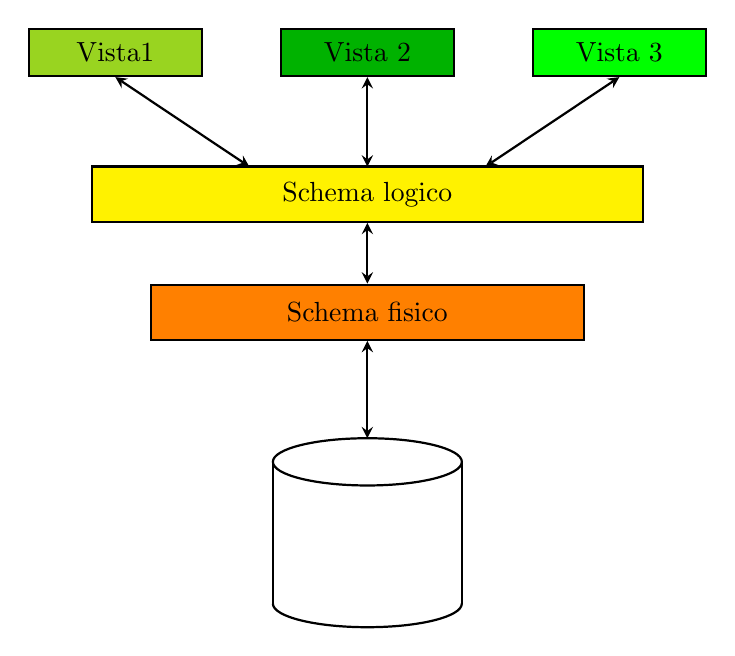
\begin{tikzpicture}[thick, >=stealth]
			
			\node[draw, fill=yellow!60!green, minimum width=2.2cm, minimum height=0.6cm] (V1) at (-3.2, 3) {Vista1};
			\node[draw, fill=green!70!black, text=black, minimum width=2.2cm, minimum height=0.6cm] (V2) at (0, 3) {Vista 2};
			\node[draw, fill=green, minimum width=2.2cm, minimum height=0.6cm] (V3) at (3.2, 3) {Vista 3};
			
			\node[draw, fill=yellow, minimum width=7cm, minimum height=0.7cm] (SL) at (0, 1.2) {Schema logico};
			
			\node[draw, fill=orange, minimum width=5.5cm, minimum height=0.7cm] (SF) at (0, -0.3) {Schema fisico};
			
			\draw (-1.2, -2.2) -- (-1.2, -4);
			\draw (1.2, -2.2) -- (1.2, -4);
			\draw (0, -2.2) ellipse (1.2 and 0.3);
			\draw (-1.2, -4) arc (180:360:1.2 and 0.3);
			
			\coordinate (DB_top) at (0, -1.9);
			
			\draw[<->] (V1.south) -- (-1.5, 1.55);
			\draw[<->] (V2.south) -- (0, 1.55);
			\draw[<->] (V3.south) -- (1.5, 1.55);
			
			\draw[<->] (SL.south) -- (SF.north);
			\draw[<->] (SF.south) -- (DB_top);
			
		\end{tikzpicture}
	\end{center}
	
	\newpage
	\section{Le transazioni}
	Un buon DBMS deve inoltre gestire anche una serie di operazioni sensibili di inserimento, modifica e cancellazione di dati, in modo che queste vengano effettuate senza contrattempi o errori.
	\begin{definizione}{Transazione}{}
		Una \textbf{transazione} è una sequenza di operazioni di lettura e scrittura in memoria che deve rispettare le seguenti proprietà \textbf{ACID}:
		\begin{itemize}
			\item \textbf{Atomicity:} deve essere una sequenza \textbf{indivisibile} di operazioni. In caso di verifica di un qualsiasi errore nel mezzo di una transazione porta questa ad essere marcata come \textit{non valida}, in quanto le operazioni devono essere eseguite \textbf{tutte o nessuna}.
			
			\item \textbf{Consistency:} bisogna lasciare i dati modificati in uno stato corretto che non viola i vincoli imposti precedentemente dal DBMS.
			
			\item \textbf{Isolation:} ogni transazione deve essere \textbf{indipendente}. Dunque durante esecuzione concorrente di più transazioni, gli effetti di una non devono dipendere dalle altre.
			
			\item \textbf{Durability:} gli effetti di una transazione devono essere \textbf{permanenti} per quanto riguarda i dati modificati (ovvero le modifiche devono necessariamente essere applicate anche su disco per mantenere la sincronizzazione dei dati).
		\end{itemize}
	\end{definizione}
	
	Vediamo di seguito un esempio di due transazioni che vengono eseguite bene o male nello stesso momento:
	
	\begin{itemize}
		\item \textbf{Transazione 1}: "Accredita 1000 € sul conto corrente $c1$"
		\item \textbf{Transazione 2}: "Accredita 500 € sul conto corrente $c1$"
	\end{itemize}
	
	Supponiamo che il valore iniziale del saldo del conto $c1$ sia pari a $2000$ €. Intuitivamente, al termine di entrambe le transazioni, ci aspetterions un valore finale di $3500$ €. Vediamo invece cosa può accadere se le operazioni vengono interlacciate nel tempo senza opportune 
	sue protezioni.
	
	\begin{osservazione}{}{}
		Una volta letto un valore, ogni transazione lo modifica nel \textbf{proprio} spazio di memoria di lavoro; altrimenti si rischiano modifiche irreversibili ai dati nello schema.
	\end{osservazione}
	
	Analizziamo la seguente tabella di esecuzione temporale delle due transazioni:
	
	\begin{tabella}{|C|C|C|}
		\hline
		\textbf{Transazione 1} & \textbf{Tempo} & \textbf{Transazione 2} \\ \hline
		cerca $c1$ & $t1$ & \\ \hline
		& $t2$ & cerca $c1$ \quad $\leftarrow$ \textit{qui non prende il valore aggiornato $+1000$} \\ \hline
		modifica \textit{saldo} in \textit{saldo}$+1000$ & $t3$ & \\ \hline
		& $t4$ & modifica \textit{saldo} in \textit{saldo}$+500$ \\ \hline
	\end{tabella}
	
	Come si può vedere dalla tabella, l'esecuzione concorrente di due transazioni, in questo caso, risulta in un esito errato, in quanto ogni transazione effettua modifiche sulla \textbf{sua} porzione di dati, e non su quella effettivamente memorizzata, il che causa problemi di sincronizzazione.
	
	\begin{definizione}{Serializzabilità}{}
		Nel caso di esecuzioni concorrenti di più transazioni, l'effetto complessivo deve essere equivalente a quello di un'esecuzione seriale, ovvero con le transazioni eseguite \textit{una dopo l'altra}, senza alcun interfogliamento delle loro operazioni elementari.
	\end{definizione}
	
	Chiaramente la serializzabilità non è sempre semplice da implementare, e si fa infatti uso di protocolli progettati per garantire a priori la correttezza di qualunque schedule di transazioni che li adottano. Queste tecniche e protocolli non saranno tuttavia argomento di questo corso, per cui si lascia al lettore la voglia di approfondire.
	
	Continuando l'analisi delle funzionalità offerte da un DBMS, è fondamentale esaminare gli strumenti messi a disposizione per la gestione e lo sviluppo. Tali funzionalità non si rivolgono unicamente agli utenti finali che eseguono interrogazioni sui dati, ma coprono ruoli cruciali come l'amministratore della base di dati e lo sviluppatore di applicazioni.
	
	Concludendo questo capitolo, se volessimo elencare i vantaggi e gli svantaggi nell'utilizzo di un DBMS \textit{ben progettato} per la memorizzazione dei dati, otterremmo un simile resoconto.
	\begin{osservazione}{Vantaggi nell'uso di un DBMS}{}
		\begin{enumerate}
			\item Indipendenza fisica e logica tra dati e applicazioni che li usano.
			
			\item Memorizzazione e recupero efficiente dei dati.
			
			\item Vincoli di integrità sui dati.
		\end{enumerate}
	\end{osservazione}	
	
	Il principale \textbf{svantaggio} nell'utilizzo di un DBMS risiede nella stretta necessità di definire uno schema di dati prima di poterli memorizzare. Tale punto diventa uno svantaggio nel momento in cui si vogliono memorizzare, ad esempio, piccole quantità di dati (ad esempio se vogliamo memorizzare il contenuto di un libro), oppure non ci interessa \textit{come} questi dati vengano memorizzati.
	
	\chapter{Progettazione di basi di dati}
	
	Progettare una base di dati significa progettare sia la \textbf{struttura dei dati} sia le \textbf{applicazioni} che vi operano sopra. Tra queste due componenti, la \textbf{progettazione dei dati} rappresenta l'attività più importante e delicata.
	Tale progettazione non è un'attività fine a sé stessa, bensì rientra nel \textbf{ciclo di vita di un sistema informativo}.
	
	\begin{definizione}{Ciclo di vita di un sistema informativo}{}
		Il \textit{ciclo di vita di un sistema informativo} è quella sequenza di attività svolte da analisti, progettisti e utenti nello sviluppo dei sistemi informativi.
		Viene detto \textit{ciclo} in quanto ogni fase non è una tantum, bensì può essere ripetuta più volte apportando le opportune modifiche al fine di raggiungere il risultato finale sperato.\\
		\linebreak
		Tale ciclo si articola nelle seguenti fasi:
		\begin{enumerate}
			\item \textbf{Studio di fattibilità:} definizione delle proprietà, stime dei costi, valutazione dei tempi richiesti dal progetto.
			
			\item \textbf{Raccolta e analisi dei requisiti}
			
			\item \textbf{Progettazione e implementazione:} modellazione concettuale e logica dei dati che si vogliono memorizzare e implementazione tramite un apposito linguaggio DBMS.
			
			\item \textbf{Validazione e collaudo:} effettuazione dei test per verificare che il sistema risponda correttamente alle esigenze.
		\end{enumerate}
	\end{definizione}
	
	La modellazione di una base di dati si colloca a \textit{metà} tra la raccolta e l'analisi dei requisiti e la progettazione effettiva.
	
	\section{Modelli informatici}
	Prima di modellare la base di dati, bisogna decidere a quale modello informatico/matematico rifarsi per la memorizzazione di questi.
	Un modello deve presentare le seguenti caratteristiche:
	\begin{itemize}
		\item Deve essere \textbf{la rappresentazione di un certo fatto concreto}.
		
		\item Tale rappresentazione deve essere descritta mediante un \textbf{linguaggio formale} (dunque che segue delle regole ben definite).
		
		\item Individuazione delle strutture da utilizzare per organizzare i dati di interesse e le relazioni tra questi.\\ Ad esempio, il modello relazionale di cui abbiamo discusso prima utilizza il concetto matematico di \textit{relazione} per organizzare i dati.
	\end{itemize}
	
	Possiamo definire due tipologie di modelli fondamentali nella progettazione di una base di dati:
	\begin{definizione}{Modello logico e modello concettuale}{}
		Il \textbf{modello logico} di una base di dati rappresenta la struttura dei dati e come questi vengono memorizzati. Si potrebbe dire che corrisponde allo schema logico visto precedentemente nel modello ANSI/SPARC, in quanto si colloca indipendente dalla memorizzazione fisica dei dati, ma è strettamente legato dal tipo di modello informatico che abbiamo scelto di adottare per la memorizzazione di questi.\\
		\linebreak
		Il \textbf{modello concettuale} è tutto il contrario: deve essere completamente indipendente dalle modalità di realizzazione, e ha lo scopo di rappresentare la realtà descritta dal problema, tramite un preciso linguaggio formale (ad esempio i diagrammi UML, ma anche il modello \textbf{Entity-Relationship (E-R)})
	\end{definizione}
	
	Non esiste un modello corretto: la stessa realtà può essere modellata in modi diversi a seconda dell'interpretazione che si dà al problema. Tuttavia deve essere seguito uno specifico "percorso mentale" nella progettazione di una base di dati:
	\begin{enumerate}
		\item \textbf{Aspetto ontologico:} quanto conosco del dominio del discorso? Quanto sono familiare con l'ambito di discussione?\\
		Durante questa fase, detta anche fase di \textit{analisi del problema}, devo delineare quali sono le entità la cui realtà deve essere modellata e come si relazionano tra loro.
		
		\item \textbf{Aspetto logico:} con quale concetto astratto voglio realizzare le entità del modello? (es. relazionale, gerarchico, reticolare, ...)\\
		Durante questa fase definisco le effettive relazioni tra le entità.
		
		\item \textbf{Aspetto linguistico:} con quale linguaggio formale definiamo il modello? (es. SQL/algebra relazionale)
		
		\item \textbf{Aspetto pragmatico:} come memorizzo i dati nei supporti di memorizzazione fisica?
	\end{enumerate}
	
	\section{Entità, collezioni e attributi}
	Nella descrizione delle fasi da seguire durante la progettazione di una base di dati abbiamo citato un termine importante e fondamentale nella modellazione concettuale della realtà di riferimento: \textbf{entità}.
	\begin{definizione}{Entità}{}
		Le \textit{entità} di un problema sono quegli oggetti a cui il problema dà particolare rilevanza, e dei quali ci interessa rappresentare alcuni fatti a loro associati, detti per l'appunto \textbf{attributi (o proprietà) dell'entità}.\\
		Ogni entità appartiene ad un \textbf{tipo} che ne specifica la natura. Ad esempio l'entità \texttt{Studente} appartiene alla categoria \texttt{Persona} (possiamo vederla come l'ereditarietà nella programmazione ad oggetti).\\
		Una \textbf{collezione} di entità è invece un insieme variabile nel tempo di entità tutte dello stesso tipo. Ad esempio, se pensiamo a tutti gli studenti di un'università, quella rappresenta una collezione di entità di tipo \texttt{Studente}.\\
		\smallbreak
		Supponiamo di dover creare la base di dati di un sistema di memorizzazione degli studenti, professori ed esami. Possiamo individuare nello studente un'\textbf{entità}, in quanto si tratta di uno degli oggetti fondamentali descritti dal problema, e nella sua matricola, cognome e data di nascita gli \textbf{attributi} fondamentali che lo descrivono.
	\end{definizione}
	
	Un entità o un attributo non mantengono il loro status costantemente all'interno di ogni analisi e di ogni problema: in una realtà potrebbe essere messa più importanza su un oggetto, spingendoci dunque a farlo diventare entità, mentre in un'altra tale importanza potrebbe mancare, rilegando così l'oggetto ad un semplice attributo.
	Ad esempio, proviamo a rappresentare una biblioteca: se ci interessasse modellare solo i libri, senza curarci degli autori, potremmo avere uno schema logico di questo tipo \texttt{Libro(titolo, annoDiPubblicazione, casaEditrice, autore)}. Se invece fossimo interessati anche agli autori, renderemmo quell'oggetto una vera e propria entità con nome e cognome, anziché lasciarlo un semplice attributo.
	
	\section{Le associazioni}
	\begin{definizione}{Associazione}{}
		Un'\textbf{istanza di associazione} è un fatto che collega due o più entità, stabilendo un legame logico fra loro.\\
		Matematicamente, definiamo $R(X, Y)$ un'associazione fra due collezioni di entità $X$ ed $Y$ un insieme di istanze di associazione tra elementi $x \in X$ e $y \in Y$. Il prodotto cartesiamo $X \times Y$ è detto \textbf{dominio dell'associazione}.\\
		\smallbreak
		Generalmente, nella modellazione concettuale, le associazioni sono descritte da un \textit{verbo} che lega le varie entità coinvolte. Chiaramente tale verbo deve essere esplicativo della natura dell'associazione, e per tale ragione si devono evitare verbi come "essere" o "avere" oppure verbi modali.\\
		Un esempio di associazione possiamo vederlo anche con il precedente esempio della biblioteca: le entità \texttt{Libro} e \texttt{Autore} sono collegate tra loro dall'associazione \texttt{SCRIVERE}, in quanto è l'autore a scrivere il libro, e il libro viene scritto dall'autore.
	\end{definizione}
	
	Un'associazione è caratterizzata dalle seguenti proprietà strutturali:
	\begin{itemize}
		\item \textbf{Molteplicità:} prese le due collezioni di entità $X$ ed $Y$ e un'associazione $R(X, Y)$, indica quante istanze di un elemento $x \in X$ sono associate ad uno e un solo elemento $y \in Y$.\\
		Formalmente, tale proprietà è descritta dal \textbf{vincolo di univocità}:
		\begin{itemize}
			\item Un'associazione si dice \textbf{univoca} rispetto ad $X$ se per ogni elemento $x \in X$ esiste \textbf{al più} un elemento $y \in Y$ che è associato ad $x$.
			
			\item Se tale vincolo fallisce (ovvero se esiste \textbf{almeno} un elemento $x \in X$ a cui è associato più di un elemento $y \in Y$) l'associazione si dice \textbf{multivalore}.
		\end{itemize}
		
		Facendo un esempio, un'associazione del tipo $R(X, Y) = (1:N)$ è multivalore su $X$ e univoca su $Y$. Viceversa, se avessimo scritto $R(X, Y) = (N:1)$, sarebbe stata univoca su $X$ e multivalore su $Y$. Possiamo leggerla "a croce", diciamo: la molteplicità dell'elemento più a sinistra è il valore più a destra, mentre quella dell'elemento più a destra è il valore più a sinistra. Come nelle proporzioni, gli esterni vanno con gli esterni e gli interni con gli interni.
		
		\item \textbf{Totalità:} indica se l'associazione tra un elemento $x \in X$ e un elemento $y \in Y$ è opzionale oppure no. Formalmente:
		\begin{itemize}
			\item Un'associazione $R(X,Y)$ si dice \textbf{totale} se, per ogni elemento $x \in X$ esiste \textit{almeno} un elemento $y \in Y$ associato ad $x$ (questa proprietà è conosciuta meglio come \textbf{obbligatorietà del valore}).
			
			\item Tale associazione si dice invece \textbf{parziale} quando il vincolo imposto precedentemente fallisce, ovvero quando ad un valore $x \in X$ \textit{non è detto} che vi sia associato un valore $y \in Y$ (questa proprietà è più conosciuta come \textbf{opzionalità}).
		\end{itemize}
		
		Ad esempio, pensiamo ad un'associazione del tipo \texttt{Possedere(Persona, AutomobileConTarga)}. Riprendendo il discorso sulla molteplicità, questa sarà del tipo \texttt{(1:N)}, in quanto una persona può possedere più di un'automobile con targa, però una singola automobile con targa è posseduta da una sola persona. Vedendo invece il vincolo di totalità, quest'associazione risulta essere \textit{opzionale} sulla Persona, in quanto non è detto che una persona possegga un'automobile, mentre è \textit{totale} su automobile, in quanto un'automobile già targata è sicuramente proprietà di qualcuno.
	\end{itemize}
	
	Vediamo adesso una delle numerose rappresentazioni grafiche con cui possiamo rappresentare le associazioni, e delle particolarità che le contraddistinguono:
	
	\begin{figure}[htbp]
		
		\begin{minipage}[c]{0.6\textwidth}
			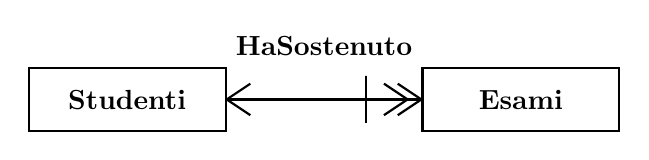
\begin{tikzpicture}[thick, baseline=(current bounding box.center)]
				
				\node[draw, minimum width=2.5cm, minimum height=0.8cm] (stud) at (0, 0) {\textbf{Studenti}};
				\node[draw, minimum width=2.5cm, minimum height=0.8cm] (esam) at (5, 0) {\textbf{Esami}};
				
				
				\draw (stud) -- (esam) node[midway, above=12pt] {\textbf{HaSostenuto}};
				
				
				\draw (stud.east) -- ++(0.3, 0.2);
				\draw (stud.east) -- ++(0.3, -0.2);
				
				
				\draw ([xshift=-20pt]esam.west) -- ++(0, 0.3) -- ++(0, -0.6);
				\draw ([xshift=0pt]esam.west) -- ++(-0.3, 0.2);
				\draw ([xshift=0pt]esam.west) -- ++(-0.3, -0.2);
				\draw ([xshift=-5pt]esam.west) -- ++(-0.3, 0.2);
				\draw ([xshift=-5pt]esam.west) -- ++(-0.3, -0.2);
				
			\end{tikzpicture}
		\end{minipage}\hfill
		\begin{minipage}[c]{0.35\textwidth}
			\caption{Relazione \textbf{HaSostenuto}}
			\label{fig:studenti_esami}
		\end{minipage}
	\end{figure}
	
	\vspace{1cm}
	
	\begin{figure}[htbp]
		\begin{minipage}[c]{0.6\textwidth}
			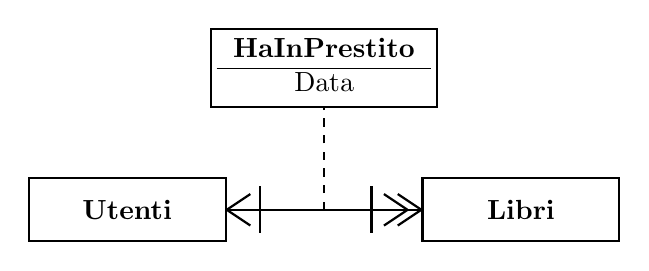
\begin{tikzpicture}[thick, baseline=(current bounding box.center)]
				
				\node[draw, minimum width=2.5cm, minimum height=0.8cm] (ute) at (0, 0) {\textbf{Utenti}};
				\node[draw, minimum width=2.5cm, minimum height=0.8cm] (lib) at (5, 0) {\textbf{Libri}};
				
				
				\node[draw, inner sep=2pt] (prestito) at (2.5, 1.8) {
					\begin{tabular}{c}
						\textbf{HaInPrestito} \\
						\hline
						Data
					\end{tabular}
				};
				
				
				\draw (ute) -- (lib);
				\draw[dashed] (2.5, 0) -- (prestito.south);
				
				
				\draw ([xshift=12pt]ute.east) -- ++(0, 0.3) -- ++(0, -0.6); 
				\draw (ute.east) -- ++(0.3, 0.2);
				\draw (ute.east) -- ++(0.3, -0.2);
				
				
				\draw ([xshift=-18pt]lib.west) -- ++(0, 0.3) -- ++(0, -0.6); 
				\draw (lib.west) -- ++(-0.3, 0.2);
				\draw (lib.west) -- ++(-0.3, -0.2);
				\draw ([xshift=-5pt]lib.west) -- ++(-0.3, 0.2);
				\draw ([xshift=-5pt]lib.west) -- ++(-0.3, -0.2);
			\end{tikzpicture}
		\end{minipage}\hfill
		\begin{minipage}[c]{0.35\textwidth}
			\caption{Relazione con attributi. L'attributo \textit{Data} è agganciato alla relazione stessa.}
			\label{fig:utenti_libri}
		\end{minipage}
	\end{figure}
	
	\vspace{1cm}
	
	\begin{figure}[htbp]
		\begin{minipage}[c]{0.6\textwidth}
			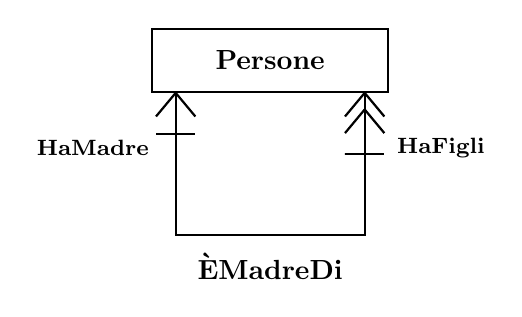
\begin{tikzpicture}[thick, baseline=(current bounding box.center)]
				
				\node[draw, minimum width=3cm, minimum height=0.8cm] (pers) at (0, 0) {\textbf{Persone}};
				
				
				\coordinate (c1) at ([xshift=-1.2cm]pers.south);
				\coordinate (c2) at ([xshift=1.2cm]pers.south);
				
				
				\draw (c1) -- ++(0, -1.8) coordinate (botLeft) 
				-- (botLeft -| c2) coordinate (botRight) node[midway, below=3pt, font=\bfseries] {ÈMadreDi}
				-- (c2);
				
				
				\node[left=6pt, font=\footnotesize\bfseries] at ([yshift=-0.7cm]c1) {HaMadre};
				\node[right=8pt, font=\footnotesize\bfseries] at ([yshift=-0.7cm]c2) {HaFigli};
				
				
				\draw ([yshift=-15pt]c1) -- ++(-0.25, 0) -- ++(0.5, 0); 
				\draw (c1) -- ++(-0.25, -0.3);
				\draw (c1) -- ++(0.25, -0.3);
				
				
				
				\draw (c2) -- ++(-0.25, -0.3);
				\draw (c2) -- ++(0.25, -0.3);
				\draw ([yshift=-6pt]c2) -- ++(-0.25, -0.3);
				\draw ([yshift=-6pt]c2) -- ++(0.25, -0.3);
				
				\draw ([yshift=-22pt]c2) -- ++(-0.25, 0) -- ++(0.5, 0); 
			\end{tikzpicture}
		\end{minipage}\hfill
		\begin{minipage}[c]{0.35\textwidth}
			\caption{Relazione ricorsiva. L'entità \textbf{Persone} si relaziona con sé stessa tramite i ruoli \textit{HaMadre} e \textit{HaFigli}.}
			\label{fig:persone_madre}
		\end{minipage}
	\end{figure}
	
	Descriviamo adesso tutte le informazioni ricavabili dalla notazione presa in esempio:
	\begin{itemize}
		\item Il singolo \texttt{>} oppure \texttt{<} significa che la relazione è \textbf{univoca} verso quel lato. Vedendo la figura \ref{fig:studenti_esami} vediamo come in questa specifica modellazione un esame venga sostenuto da uno e un singolo studente.
		
		\item Il doppio \texttt{>>} oppure \texttt{<<} significa che da quel lato la relazione è \textbf{multivalore}. Sempre prendendo in esempio gli studenti, uno studente può aver sostenuto più volte lo stesso esame. Anche con \texttt{Utenti - Libri}, vediamo come un utente prende in presito più libri, mentre un libro viene preso in prestito solo da un utente alla volta.
		
		\item La barra verticale \texttt{|} vicino alla molteplicità indica che da quel lato la relazione è \textbf{parziale}, dunque opzionale. Ad esempio vediamo come, nel caso \texttt{Studenti - Esami} il singolo studente potrebbe ancora non aver mai sostenuto quell'esame, mentre l'esame stesso, essendo registrato, è sicuramente stato sostenuto da qualche studente.
	\end{itemize}
	
	\section{Le gerarchie di classi}
	Spesso le classi di entità sono organizzate in una gerarchia di \textit{specializzazione/generalizzazione}. Una classe della gerarchia minore di altre viene detta \textbf{sottoclasse}, mentre le altre prendono il nome di \textbf{superclassi}. Il concetto è lo stesso alla base dell'ereditarietà nella programmazione ad oggetti.
	Per fare un esempio pertinente, la classe degli \textit{studenti universitari} può è una generalizzazione (o sopraclasse) delle seguenti classi:
	\begin{itemize}
		\item Matricole e laureandi.
		\item Studenti in corso e studenti fuori corso.
		\item Studenti locali e studenti fuori sede.
		\item Studenti maschi e studentesse.
	\end{itemize}
	
	Fra i tipi oggetto è definita una \textbf{relazione di sottotipo} che regola la struttura gerarchica dei dati.
	Per il lettore questa è semplicemente una formalizzazione matematica del concetto di \textit{polimorfismo} all'interno della programmazione ad oggetti.
	
	\begin{definizione}{Relazione di sottotipo}{rel_sottotipo}
		Fra i tipi oggetto viene stabilita una relazione di sottotipo che soddisfa le seguenti proprietà fondamentali:
		\begin{itemize}
			\item È \textbf{asimmetrica}, \textbf{riflessiva} e \textbf{transitiva} (definendo così una relazione di ordine parziale).
			\item \textbf{Principio di sostitutività}: Se $T$ è sottotipo di $T'$, allora gli elementi appartenenti al tipo $T$ possono essere usati in qualsiasi contesto in cui possano apparire valori di tipo $T'$.
			
			In particolare, ciò implica che:
			\begin{itemize}
				\item Gli elementi di $T$ possiedono tutte le proprietà degli elementi di $T'$.
				\item Per ogni proprietà $p$ in $T'$, il suo tipo associato in $T$ deve essere un sottotipo del suo tipo in $T'$.
			\end{itemize}
		\end{itemize}
	\end{definizione}
	
	Facendo nuovamente riferimento alla programmazione ad oggetti, anche nella modellazione concettuale possiamo definire degli oggetti (le entità del problema che vogliamo modellare) a partire da altri già esistenti. Questi nuovi oggetti erediteranno dal proprio genitore (o \textit{dai propri genitori}, in quanto viene supportata l'ereditarietà multipla) tutti i suoi attributi, e potranno anche definirne di nuovi o ridefinire gli esistenti.
	
	\begin{figure}[htbp]
		
		\begin{minipage}[c]{0.5\textwidth}
			\centering
			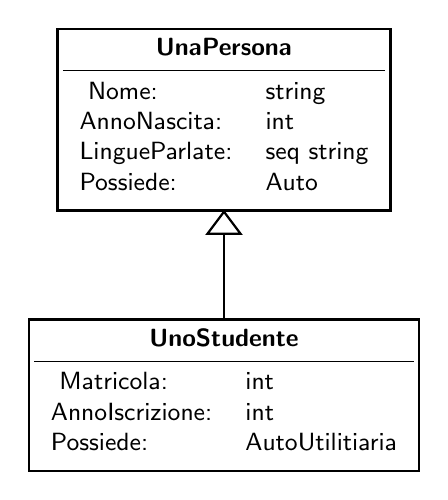
\begin{tikzpicture}[thick, baseline=(current bounding box.center)]
				
				
				\tikzset{
					classbox/.style={
						draw,
						inner sep=2pt, 
						font=\small\sffamily
					}
				}
				
				
				\node[classbox] (persona) at (0, 0) {
					\begin{tabular}{ll}
						\multicolumn{2}{c}{\textbf{UnaPersona}} \\[2pt]
						\hline
						\rule{0pt}{10pt}
						Nome: & string \\
						AnnoNascita: & int \\
						LingueParlate: & seq string \\
						Possiede: & Auto \\[2pt]
					\end{tabular}
				};
				
				
				\node[classbox] (studente) at (0, -3.5) {
					\begin{tabular}{ll}
						\multicolumn{2}{c}{\textbf{UnoStudente}} \\[2pt]
						\hline
						\rule{0pt}{10pt}
						Matricola: & int \\
						AnnoIscrizione: & int \\
						Possiede: & AutoUtilitiaria \\[2pt]
					\end{tabular}
				};
				
				\draw[fill=white] (persona.south) -- ++(-6pt, -8pt) -- ++(12pt, 0) -- cycle;
				
				\draw (studente.north) -- ([yshift=-8pt]persona.south);
				
			\end{tikzpicture}
		\end{minipage}\hfill
		\begin{minipage}[c]{0.45\textwidth}
			\caption{Ereditarietà tra classi. La classe \textbf{UnoStudente} eredita da \textbf{UnaPersona}, specializzando il tipo dell'attributo \textit{Possiede}.}
			\label{fig:ereditarieta_persona_studente}
		\end{minipage}
	\end{figure}
	
	Fra le classi può essere definita una relazione di \textbf{sottoclasse}, detta anche di \textbf{sottoinsieme}, caratterizzata dalle seguenti proprietà:
	
	\begin{definizione}{Relazione di sottoclasse}{}
		La \textbf{relazione di sottoclasse }è definita dalle seguenti proprietà:
		\begin{itemize}
			\item È \textbf{antisimmetrica}, \textbf{riflessiva} e \textbf{transitiva}.
			\item Se $C$ è sottoclasse di $C'$, allora il tipo degli elementi di $C$ è sottotipo del tipo degli elementi di $C'$ (\textbf{vincolo intensionale}).
			\item Se $C$ è sottoclasse di $C'$, allora gli elementi di $C$ sono un sottoinsieme degli elementi di $C'$ (\textbf{vincolo estensionale}).
		\end{itemize}
	\end{definizione}
	
	\subsection{Vincoli su insiemi di sottoclassi}
	Per gli insiemi delle sottoclassi (i domini dei valori che tali classi possono assumere) vengono anche stabiliti dei vincoli.
	
	\begin{definizione}{Vincolo di disgiunzione}{}
		Gli elementi di una sottoclasse non possono far parte di un'altra sottoclasse.\\
		Sostanzialmente stiamo dicendo che, avendo delle classi che sono specializzazioni di una sopraclasse, tali sottoclassi \textbf{non avranno nulla in comune}, e dunque un elemento di una sottoclasse non avrà nulla a che vedere con un elemento di un'altra sottoclasse.\\
		Pensiamo ad esempio di avere una classe \texttt{Persona} che ha come sottoclassi \texttt{Maggiorenni} e \texttt{Minorenni}. Tra queste sottoclassi vige il vincolo di disgiunzione, in quanto una persona non potrà \textbf{mai} essere contemporaneamente sia minorenne che maggiorenne.
		D'altro canto, se avessimo una classe \texttt{Persona} con sottoclassi \texttt{Programmatore} e \texttt{Maggiorenne}, tra queste due sottoclassi non vige il vincolo di disgiunzione in quanto non possiamo categoricamente dire che nessun programmatore è maggiorenne o viceversa.
		Formalizzando in maniera matematica questo vincolo, possiamo dire che \textit{i domini delle due sottoclassi sono due insiemi la cui intersezione è nulla}.
		
		\vspace{6pt}
		\begin{center}
			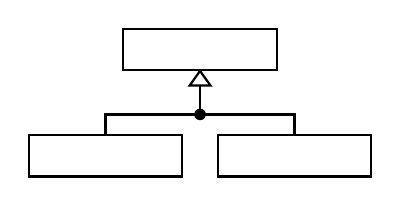
\begin{tikzpicture}[scale=0.75, transform shape, thick]
				\tikzset{
					classbox/.style={
						draw,
						minimum width=2.6cm,
						minimum height=0.7cm,
						fill=white
					}
				}
				
				
				\node[classbox] (super) at (0, 0) {};
				
				
				\node[classbox] (sub1) at (-1.6, -1.8) {};
				\node[classbox] (sub2) at (1.6, -1.8) {};
				
				
				\draw[fill=white] (super.south) -- ++(-5pt, -7pt) -- ++(10pt, 0) -- cycle;
				
				
				\coordinate (split) at (0, -1.1);
				
				
				\draw ([yshift=-7pt]super.south) -- (split);
				\fill (split) circle (2.8pt);
				
				
				\draw (split) -| (sub1.north);
				\draw (split) -| (sub2.north);
			\end{tikzpicture}
		\end{center}
	\end{definizione}
	
	\begin{definizione}{Vincolo di copertura}{}
		L'unione degli elementi delle sottoclassi contiene \textbf{tutti} gli elementi della sopraclasse.\\
		Mantenendoci sempre sull'esempio fatto in precedenza con \texttt{Persona, Maggiorenne, Minorenne}, tra le due sottoclassi è presente un vincolo di copertura, in quanto una persona \textbf{o} è maggiorenne \textbf{o} è minorenne. Necessariamente una delle due.
		In modo più matematico e formale, possiamo dire che \textit{l'unione dei domini delle sottoclassi è uguale al dominio della sopraclasse}.
		
		\vspace{6pt}
		\begin{center}
			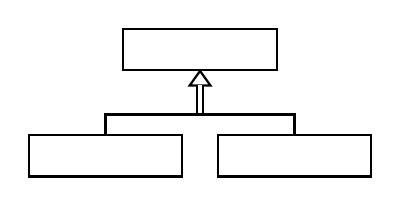
\begin{tikzpicture}[scale=0.75, transform shape, thick]
				\tikzset{
					classbox/.style={
						draw,
						minimum width=2.6cm,
						minimum height=0.7cm,
						fill=white
					}
				}
				
				
				\node[classbox] (super) at (0, 0) {};
				
				
				\node[classbox] (sub1) at (-1.6, -1.8) {};
				\node[classbox] (sub2) at (1.6, -1.8) {};
				
				
				\draw[fill=white] (super.south) -- ++(-5pt, -7pt) -- ++(10pt, 0) -- cycle;
				
				
				\coordinate (split) at (0, -1.1);
				
				
				\draw[double, double distance=1.2pt] ([yshift=-7pt]super.south) -- (split);
				
				
				\draw (split) -| (sub1.north);
				\draw (split) -| (sub2.north);
			\end{tikzpicture}
		\end{center}
	\end{definizione}
	
	Se tra le sottoclassi di una gerarchia si verificano contemporaneamente il vincolo di disgiunzione e quello di copertura, si dice che l'insieme delle sottoclassi è una \textbf{partizione} della classe padre.
	
	\section{Le fasi per la costruzione di una base di dati}
	
	Il ciclo di vita e il processo di sviluppo di una base di dati si articola nelle seguenti fasi principali:
	
	\begin{itemize}
		\item \textbf{Analisi dei requisiti}: consiste nell'analizzare il problema e comprenderne a fondo le specifiche fornite dall'utente o committente, tipicamente in linguaggio naturale.
		
		\item \textbf{Progettazione}: si suddivide a sua volta nella progettazione dei dati e nella progettazione delle applicazioni.
		\begin{itemize}
			\item \textbf{Progettazione concettuale}: ha lo scopo di individuare le entità di interesse e le associazioni tra di esse, formalizzandole tramite un apposito modello concettuale ad alto livello (ad esempio il modello E-R o i diagrammi delle classi UML) che serve a descrivere la realtà di riferimento da un punto di vista abbastanza astratto, in maniera totalmente indipendente da quella con cui saranno organizzati i dati dal DBMS.
			
			\item \textbf{Progettazione logica}: consiste nella traduzione dello schema concettuale nel modello logico scelto (ad esempio il modello relazionale), definendo puntualmente le strutture dati logiche e le relazioni intercorrenti tra esse.
			
			\item \textbf{Progettazione fisica dei dati}: riguarda gli aspetti implementativi di basso livello, definendo l'organizzazione fisica e le strutture di memorizzazione dei dati su disco (file di memorizzazione, indici, metodi di accesso).
			
			\item \textbf{Progettazione delle applicazioni}: definizione dell'architettura e della logica dei programmi software che interagiranno con la base di dati.
		\end{itemize}
		
		\item \textbf{Realizzazione}: fase in cui il database viene effettivamente implementato sul DBMS prescelto, popolato e integrato con le applicazioni software.
	\end{itemize}
	
	\chapter{Progettazione concettuale}
	Nel corso del seguente capitolo analizzeremo la prima fase della progettazione di una base di dati, forse la più fondamentale, che ci permetterà di tracciare le basi per la creazione delle relazioni e delle tabelle in memoria.
	
	Durante la fase di progettazione concettuale, in cui si va a delineare il \textbf{modello concettuale} derivato dall'analisi del problema, è prevalente l'\textbf{aspetto intensionale della progettazione}.
	\begin{definizione}{Aspetto intensionale}{}
		L'aspetto intensionale è quel lato della progettazione che definisce quali entità esistono, quali attributi hanno e quali vincoli devono rispettare. E' \textbf{invariante nel tempo}.
	\end{definizione}
	Il modello concettuale più diffuso è sicuramente il \textbf{modello E-R}, del quale parleremo maggiormente nella prossima sezione.
	
	\section{Il modello E-R}
	Il modello E-R è un modello grafico utilizzato per descrivere la struttura astratta di una base di dati, indicando gli oggetti coinvolti e le relazioni tra questi.
	Mette le basi su alcuni costrutti fondamentali.
	
	\subsection{Entità}
	\begin{definizione}{Entità}{}
		\textbf{Classi di oggetti omogenei tra loro e con esistenza autonoma}. Ciò vuol dire che un'entità, per esistere, non deve essere necessariamente collegata o dipendente da qualcos'altro. Sono, insieme alle associazioni, l'aspetto più importante del problema, dato che, informalmente parlando, le entità si trasformeranno nelle \textit{tabelle} durante la progettazione del modello logico. Un esempio di entità potrebbe essere un \texttt{Professore} o un \texttt{Corso} nell'ottica di una base di dati universitaria. L'entità è quell'oggetto a cui, nella descrizione della realtà di riferimento, si attribuisce particolare importanza e a cui è richiesto che vengano fatte afferire delle informazioni (gli attributi).
		\smallbreak
		Ogni entità ha un \textbf{nome identificativo} (che può essere qualsiasi, ma ovviamente si tende a scegliere nomi che facciano capire cosa si sta modellando) che per convenzione si scrive al \textbf{singolare}.
	\end{definizione}
	E' importante distinguere il concetto di entità da quello di \textbf{istanza}, in quanto quest'ultima non rappresenta una classe di oggetti dello stesso tipo bensì \textbf{il singolo oggetto, il singolo elemento della classe}.
	Nel modello concettuale rappresentiamo le entità, non le singole istanze.
	
	\begin{figure}[htbp]
		\centering
		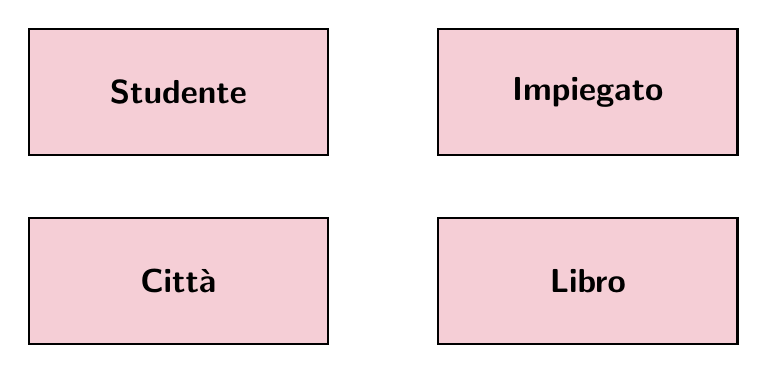
\begin{tikzpicture}[thick]
			
			% Definizione del colore rosa chiaro dei blocchi
			\definecolor{softpink}{RGB}{245, 206, 214}
			
			% Stile per le entità
			\tikzset{
				entity/.style={
					draw,
					fill=softpink,
					minimum width=3.8cm,
					minimum height=1.6cm,
					font=\sffamily\bfseries\large,
					align=center
				}
			}
			
			% Griglia 2x2 delle entità
			\node[entity] (studente)  at (0, 2.4)   {Studente};
			\node[entity] (impiegato) at (5.2, 2.4) {Impiegato};
			\node[entity] (citta)     at (0, 0)     {Città};
			\node[entity] (libro)     at (5.2, 0)   {Libro};
			
		\end{tikzpicture}
		\caption{Un esempio della rappresentazione grafica delle entità nel modello E-R}
		\label{fig:entita_grafica}
	\end{figure}
	
	\subsection{Associazioni}
	\begin{definizione}{Associazione}{etichetta}
		Legame logico che si stabilisce tra due o più entità che hanno qualcosa in comune. Queste \textit{non} sono autonome, in quanto affinché esista un'associazione è necessario ci siano almeno 2 entità coinvolte in questa. Mantenendo l'esempio di \texttt{Professore} e \texttt{Corso}, un'associazione che li lega potrebbe essere \texttt{Insegnamento}. 
		\smallbreak
		A seconda della convenzione utilizzata, le associazioni potrebbero essere indicate da un sostantivo oppure da un verbo.
	\end{definizione}
	Anche qui, è importante distinguere tra associazione e \textbf{occorrenza}, in quanto quest'ultima individua il singolo elemento della classe di legami, identificato dalle istanze delle entità che collega.
	In generale un'associazione si dice \textbf{n-aria} quando collega contemporaneamente $n$ entità.
	
	\begin{figure}[htbp]
		\centering
		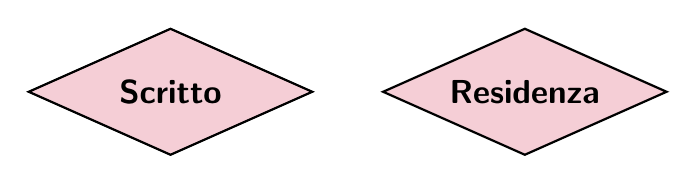
\begin{tikzpicture}[thick]
			
			% Colore coerente con i diagrammi E-R precedenti
			\definecolor{softpink}{RGB}{245, 206, 214}
			
			% Dimensioni per i rombi (semidiametro orizzontale e verticale)
			\def\rx{1.8}
			\def\ry{0.8}
			
			% -------------------------------------------------------------
			% 1. Relazione "Scritto" (a sinistra)
			% -------------------------------------------------------------
			\coordinate (c1) at (0, 0);
			\draw[fill=softpink] (c1) ++(0, \ry) -- ++(\rx, -\ry) -- ++(-\rx, -\ry) -- ++(-\rx, \ry) -- cycle;
			\node[font=\sffamily\bfseries\large] at (c1) {Scritto};
			
			% -------------------------------------------------------------
			% 2. Relazione "Residenza" (a destra)
			% -------------------------------------------------------------
			\coordinate (c2) at (4.5, 0);
			\draw[fill=softpink] (c2) ++(0, \ry) -- ++(\rx, -\ry) -- ++(-\rx, -\ry) -- ++(-\rx, \ry) -- cycle;
			\node[font=\sffamily\bfseries\large] at (c2) {Residenza};
			
		\end{tikzpicture}
		\caption{Rappresentazione grafica di associazioni senza le entità coinvolte.}
		\label{fig:relazioni_rombi}
	\end{figure}
	
	Vediamo adesso alcune categorie particolari di associazioni che si potrebbero incontrare nella scrittura del modello E-R.
	
	\begin{figure}[htbp]
		\centering
		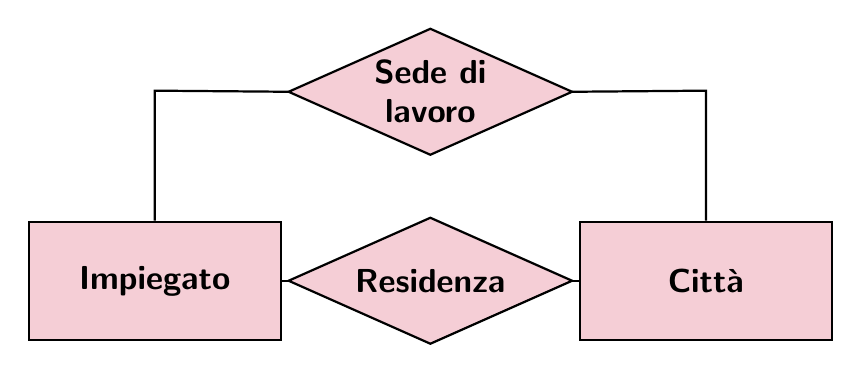
\begin{tikzpicture}[thick]
			\definecolor{softpink}{RGB}{245, 206, 214}
			
			\def\rx{1.8}
			\def\ry{0.8}
			
			% Entità: Impiegato e Città
			\node[draw, fill=softpink, minimum width=3.2cm, minimum height=1.5cm, font=\sffamily\bfseries\large] (imp) at (0, 0) {Impiegato};
			\node[draw, fill=softpink, minimum width=3.2cm, minimum height=1.5cm, font=\sffamily\bfseries\large] (cit) at (7, 0) {Città};
			
			% Relazione inferiore: Residenza
			\coordinate (cRes) at (3.5, 0);
			\draw[fill=softpink] (cRes) ++(0, \ry) -- ++(\rx, -\ry) -- ++(-\rx, -\ry) -- ++(-\rx, \ry) -- cycle;
			\node[font=\sffamily\bfseries\large] at (cRes) {Residenza};
			
			% Relazione superiore: Sede di lavoro
			\coordinate (cSed) at (3.5, 2.4);
			\draw[fill=softpink] (cSed) ++(0, \ry) -- ++(\rx, -\ry) -- ++(-\rx, -\ry) -- ++(-\rx, \ry) -- cycle;
			\node[font=\sffamily\bfseries\large, align=center] at (cSed) {Sede di\\lavoro};
			
			% Collegamenti della relazione Residenza
			\draw (imp.east) -- ([xshift=-\rx cm]cRes);
			\draw ([xshift=\rx cm]cRes) -- (cit.west);
			
			% Collegamenti della relazione Sede di lavoro
			\draw (imp.north) -- ++(0, 1.65) -- ([xshift=-\rx cm]cSed);
			\draw (cit.north) -- ++(0, 1.65) -- ([xshift=\rx cm]cSed);
		\end{tikzpicture}
		\caption{Multiple associazioni sulle stesse entità}
		\label{fig:impiegato_citta_relazioni}
	\end{figure}
	
	\begin{figure}[htbp]
		\centering
		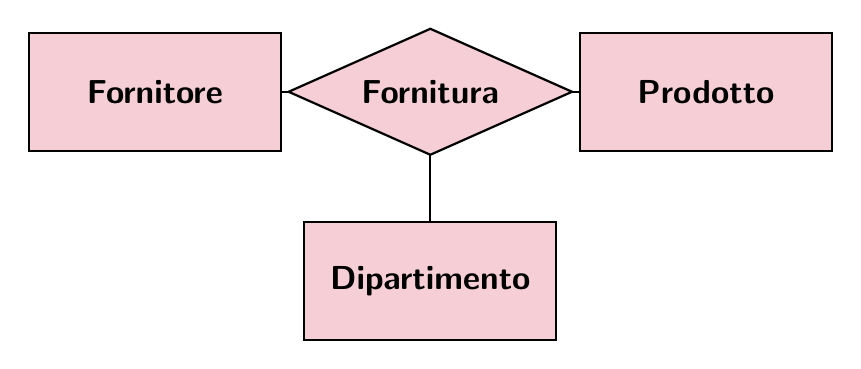
\begin{tikzpicture}[thick]
			\definecolor{softpink}{RGB}{245, 206, 214}
			
			\def\rx{1.8}
			\def\ry{0.8}
			
			% Entità: Fornitore, Prodotto e Dipartimento
			\node[draw, fill=softpink, minimum width=3.2cm, minimum height=1.5cm, font=\sffamily\bfseries\large] (forn) at (0, 0) {Fornitore};
			\node[draw, fill=softpink, minimum width=3.2cm, minimum height=1.5cm, font=\sffamily\bfseries\large] (prod) at (7, 0) {Prodotto};
			\node[draw, fill=softpink, minimum width=3.2cm, minimum height=1.5cm, font=\sffamily\bfseries\large] (dip)  at (3.5, -2.4) {Dipartimento};
			
			% Relazione ternaria: Fornitura
			\coordinate (cForn) at (3.5, 0);
			\draw[fill=softpink] (cForn) ++(0, \ry) -- ++(\rx, -\ry) -- ++(-\rx, -\ry) -- ++(-\rx, \ry) -- cycle;
			\node[font=\sffamily\bfseries\large] at (cForn) {Fornitura};
			
			% Collegamenti della relazione ternaria
			\draw (forn.east) -- ([xshift=-\rx cm]cForn);
			\draw ([xshift=\rx cm]cForn) -- (prod.west);
			\draw ([yshift=-\ry cm]cForn) -- (dip.north);
		\end{tikzpicture}
		\caption{Associazione n-aria (in questo caso ternaria).}
		\label{fig:relazione_ternaria_fornitura}
	\end{figure}
	
	\begin{figure}[htbp]
		\centering
		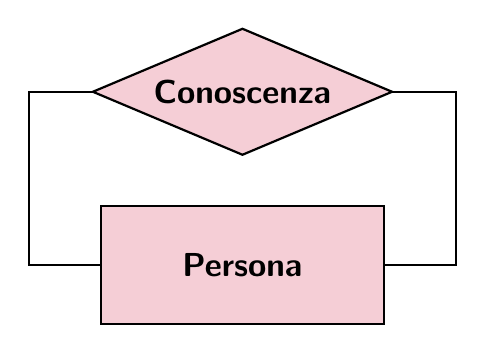
\begin{tikzpicture}[thick]
			\definecolor{softpink}{RGB}{245, 206, 214}
			
			\def\rx{1.9}
			\def\ry{0.8}
			
			% Entità: Persona
			\node[draw, fill=softpink, minimum width=3.6cm, minimum height=1.5cm, font=\sffamily\bfseries\large] (pers) at (0, 0) {Persona};
			
			% Relazione ricorsiva: Conoscenza
			\coordinate (cCon) at (0, 2.2);
			\draw[fill=softpink] (cCon) ++(0, \ry) -- ++(\rx, -\ry) -- ++(-\rx, -\ry) -- ++(-\rx, \ry) -- cycle;
			\node[font=\sffamily\bfseries\large] at (cCon) {Conoscenza};
			
			% Collegamenti ad anello della relazione ricorsiva
			\draw (pers.west) -- ++(-0.9, 0) |- ([xshift=-\rx cm]cCon);
			\draw (pers.east) -- ++(0.9, 0) |- ([xshift=\rx cm]cCon);
		\end{tikzpicture}
		\caption{Associazione ricorsiva, cioè che coinvolge un'entità con sé stessa.}
		\label{fig:relazione_ricorsiva_conoscenza}
	\end{figure}
	
	\newpage
	\subsection{Attributi}
	\begin{definizione}{Attributo}{}
		Proprietà elementare, caratteristica di un'entità o di un'associazione. Si potrebbe pensare agli attributi del modello concettuale in modo similare agli attributi di classe nella programmazione ad oggetti.
	\end{definizione}
	
	\begin{figure}[htbp]
		\centering
		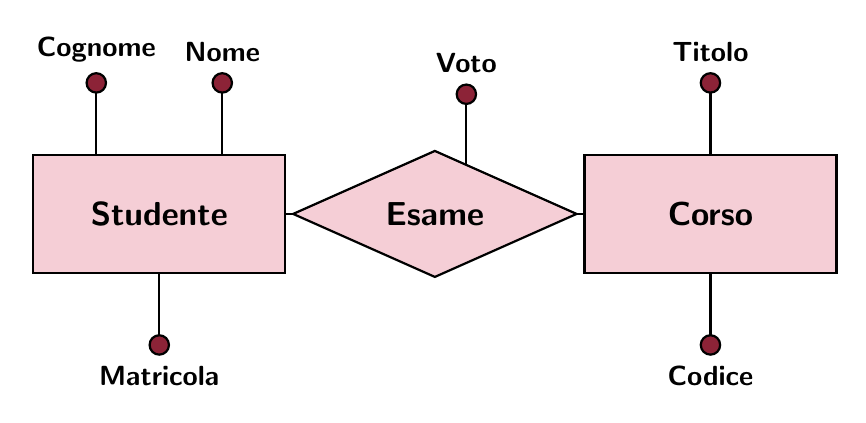
\begin{tikzpicture}[thick]
			\definecolor{softpink}{RGB}{245, 206, 214}
			\definecolor{darkred}{RGB}{140, 35, 55}
			
			\def\rx{1.8}
			\def\ry{0.8}
			
			% Entità: Studente e Corso
			\node[draw, fill=softpink, minimum width=3.2cm, minimum height=1.5cm, font=\sffamily\bfseries\large] (stud) at (0, 0) {Studente};
			\node[draw, fill=softpink, minimum width=3.2cm, minimum height=1.5cm, font=\sffamily\bfseries\large] (corso) at (7, 0) {Corso};
			
			% Relazione: Esame
			\coordinate (cEsame) at (3.5, 0);
			\draw[fill=softpink] (cEsame) ++(0, \ry) -- ++(\rx, -\ry) -- ++(-\rx, -\ry) -- ++(-\rx, \ry) -- cycle;
			\node[font=\sffamily\bfseries\large] at (cEsame) {Esame};
			
			% Collegamento tra entità e relazione
			\draw (stud.east) -- ([xshift=-\rx cm]cEsame);
			\draw ([xshift=\rx cm]cEsame) -- (corso.west);
			
			% Attributi di Studente
			\draw ([xshift=-0.8cm]stud.north) -- ++(0, 0.9) coordinate (aCognome);
			\filldraw[fill=darkred] (aCognome) circle (3.5pt) node[above=4pt, font=\sffamily\bfseries\normalsize] {Cognome};
			
			\draw ([xshift=0.8cm]stud.north) -- ++(0, 0.9) coordinate (aNome);
			\filldraw[fill=darkred] (aNome) circle (3.5pt) node[above=4pt, font=\sffamily\bfseries\normalsize] {Nome};
			
			\draw (stud.south) -- ++(0, -0.9) coordinate (aMatr);
			\filldraw[fill=darkred] (aMatr) circle (3.5pt) node[below=4pt, font=\sffamily\bfseries\normalsize] {Matricola};
			
			\draw ([xshift=0.4cm, yshift=0.62cm]cEsame) -- ++(0, 0.9) coordinate (aVoto);
			\filldraw[fill=darkred] (aVoto) circle (3.5pt) node[above=4pt, font=\sffamily\bfseries\normalsize] {Voto};
			
			% Attributi di Corso
			\draw (corso.north) -- ++(0, 0.9) coordinate (aTitolo);
			\filldraw[fill=darkred] (aTitolo) circle (3.5pt) node[above=4pt, font=\sffamily\bfseries\normalsize] {Titolo};
			
			\draw (corso.south) -- ++(0, -0.9) coordinate (aCodice);
			\filldraw[fill=darkred] (aCodice) circle (3.5pt) node[below=4pt, font=\sffamily\bfseries\normalsize] {Codice};
		\end{tikzpicture}
		\caption{Modello E-R con entità, associazioni, e i loro attributi.}
		\label{fig:attributi}
	\end{figure}
	
	Gli attributi possono anche essere \textbf{composti}, cioè attributi che raggruppano più informazioni insieme. Un esempio di attributo composto potrebbe essere l'indirizzo di residenza di una persona, in quanto l'informazione indirizzo può essere ulteriormente scomposta in \textit{Via}, \textit{Numero civico} e \textit{CAP}, ad esempio.
	In un'applicazione la scelta di mantenere un attributo composto anziché suddividerlo nelle sue componenti atomiche dipende dall'importanza che quell'attributo in seguito all'analisi del problema.
	
	\subsection{Cardinalità di associazioni}
	\begin{definizione}{Cardinalità di associazioni}{}
		Si tratta di una coppia di valori che si attribuisce ad ogni entità coinvolta in un'associazione. Si tratta di una rappresentazione grafica dei concetti di \textbf{univoco} e \textbf{multivalore} visti precedentemente.
		\smallbreak
		Specificano il numero minimo e massimo di occorrenze dell'associazione a cui un'istanza della prima entità può essere collegato rispetto ad istanze della seconda entità.
	\end{definizione}
	
	Vediamo adesso più nel dettaglio le varie tipologie di cardinalità:
	\begin{itemize}
		\item \textbf{Partecipazione minima}
		\begin{itemize}
			\item \textbf{0}: indica che la partecipazione di un'istanza dell'entità di partenza all'associazione è \textbf{opzionale}. Ciò vuol dire che potrebbe esserci anche una singola occorrenza dell'entità di partenza che non è associata a nessuna occorrenza dell'entità di arrivo. E' il corrispettivo dell'associazione \textbf{parziale} che avevamo già visto.
			
			\item \textbf{1}: indica che ogni istanza dell'entità di partenza è associata ad almeno un'occorrenza dell'altra entità. E' il corrispettivo dell'associazione \textbf{totale} che avevamo già visto.
		\end{itemize}
		
		\item \textbf{Partecipazione massima}:
		\begin{itemize}
			\item \textbf{1}: indica che ogni occorrenza dell'entità di partenza è collegata al massimo ad un'occorrenza dell'entità di arrivo. E' il corrispettivo dell'associazione \textbf{univoca} che avevamo già visto.
			
			\item \textbf{N}: indica che ogni occorrenza dell'entitò di partenza può essere collegata a più occorrenze dell'entità di arrivo. E' il corrispettivo dell'associazione \textbf{multivalore} che avevamo già visto.
		\end{itemize}
	\end{itemize}
	
	Con riferimento alle cardinalità appena mostrate, possiamo distinguere varie tipologie di associazioni:
	\begin{itemize}
		\item \textbf{Uno ad uno}, si verifica quando la cardinalità dell'entità è del tipo (1, 1).
		
		\item \textbf{Uno a molti}, si verifica quando la cardinalità è del tipo (1, N).
		
		\item \textbf{Molti a molti}, si verifica quando entrambe le entità coinvolte hanno cardinalità (0, N) oppure (1, N).
	\end{itemize}
	
	\begin{figure}[H]
		\centering
		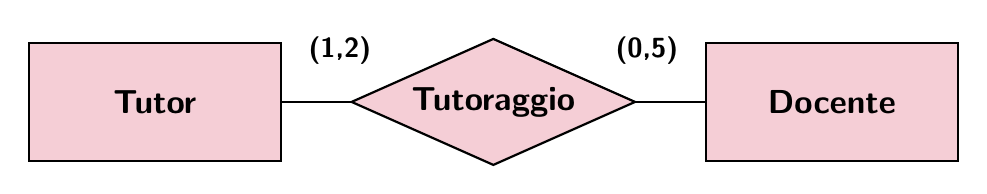
\begin{tikzpicture}[thick]
			\definecolor{softpink}{RGB}{245, 206, 214}
			
			\def\rx{1.8}
			\def\ry{0.8}
			
			% Entità: Studente e Docente
			\node[draw, fill=softpink, minimum width=3.2cm, minimum height=1.5cm, font=\sffamily\bfseries\large] (stud) at (0, 0) {Tutor};
			\node[draw, fill=softpink, minimum width=3.2cm, minimum height=1.5cm, font=\sffamily\bfseries\large] (doc)  at (8.6, 0) {Docente};
			
			% Relazione: Tutoraggio
			\coordinate (cTut) at (4.3, 0);
			\draw[fill=softpink] (cTut) ++(0, \ry) -- ++(\rx, -\ry) -- ++(-\rx, -\ry) -- ++(-\rx, \ry) -- cycle;
			\node[font=\sffamily\bfseries\large] at (cTut) {Tutoraggio};
			
			% Linee di collegamento
			\draw (stud.east) -- ([xshift=-\rx cm]cTut);
			\draw ([xshift=\rx cm]cTut) -- (doc.west);
			
			% Cardinalità (nodi separati con coordinate assolute)
			\node[font=\sffamily\bfseries] at (2.35, 0.65) {(1,2)};
			\node[font=\sffamily\bfseries] at (6.25, 0.65) {(0,5)};
		\end{tikzpicture}
		\caption{Relazione tra un tutor e un docente, che si legge nel seguente modo: Un tutor fa il tutoraggio ad 1 massimo 2 docenti. Un docente può avere da 0 a 5 tutor che fanno tutoriaggio.}
		\label{fig:tutoraggio_studente_docente}
	\end{figure}
	
	E' possibile delineare la cardinalità anche per gli attributi: quando questa non viene indicata è implicitamente (1, 1).
	\begin{figure}[H]
		\centering
		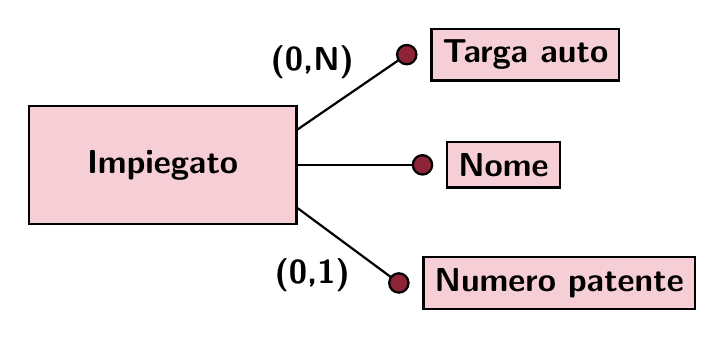
\begin{tikzpicture}[thick]
			\definecolor{softpink}{RGB}{245, 206, 214}
			\definecolor{darkred}{RGB}{140, 35, 55}			
			% Entità: Impiegato
			\node[draw, fill=softpink, minimum width=3.4cm, minimum height=1.5cm, font=\sffamily\bfseries\large] (imp) at (0, 0) {Impiegato};
			
			% Punti di aggancio degli attributi con pallino rosso scuro
			\coordinate (pTarga)   at (3.1, 1.4);
			\coordinate (pNome)    at (3.3, 0);
			\coordinate (pPatente) at (3.0, -1.5);
			
			% Linee di collegamento
			\draw (imp.east |- 0, 0.45) -- (pTarga);
			\draw (imp.east) -- (pNome);
			\draw (imp.east |- 0, -0.55) -- (pPatente);
			
			% Pallini degli attributi
			\filldraw[fill=darkred] (pTarga) circle (3.5pt);
			\filldraw[fill=darkred] (pNome) circle (3.5pt);
			\filldraw[fill=darkred] (pPatente) circle (3.5pt);
			
			% Nodi degli attributi (box rosa allineati a sinistra)
			\node[draw, fill=softpink, anchor=west, inner sep=4pt, font=\sffamily\bfseries\large] at (3.4, 1.4) {Targa auto};
			\node[draw, fill=softpink, anchor=west, inner sep=4pt, font=\sffamily\bfseries\large] at (3.6, 0) {Nome};
			\node[draw, fill=softpink, anchor=west, inner sep=4pt, font=\sffamily\bfseries\large] at (3.3, -1.5) {Numero patente};
			
			% Cardinalità separate e posizionate in modo indipendente
			\node[font=\sffamily\bfseries\large] at (1.9, 1.3) {(0,N)};
			\node[font=\sffamily\bfseries\large] at (1.9, -1.4) {(0,1)};
		\end{tikzpicture}
		\caption{Esempio di cardinalità su attributi. Come per le associazioni, scrivere 0 come cardinalità minima indica che l'attributo non è obbligatorio.}
		\label{fig:impiegato_attributi_cardinalita}
	\end{figure}
	
	\subsection{Identificatore di un'entità}
	\begin{definizione}{Identificatore}{}
		L'identificatore è quell'attributo o quell'insieme di attributi che permettono di identificare univocamente un'istanza di entità.\\
		Questi identificatori possono essere costituiti da:
		\begin{itemize}
			\item Uno o più attributi interni all'entità.
			
			\item Uno o più attributi esterni ottenuti attraverso associazioni.
		\end{itemize}
	\end{definizione}
	
	\begin{figure}[htbp]
		\centering
		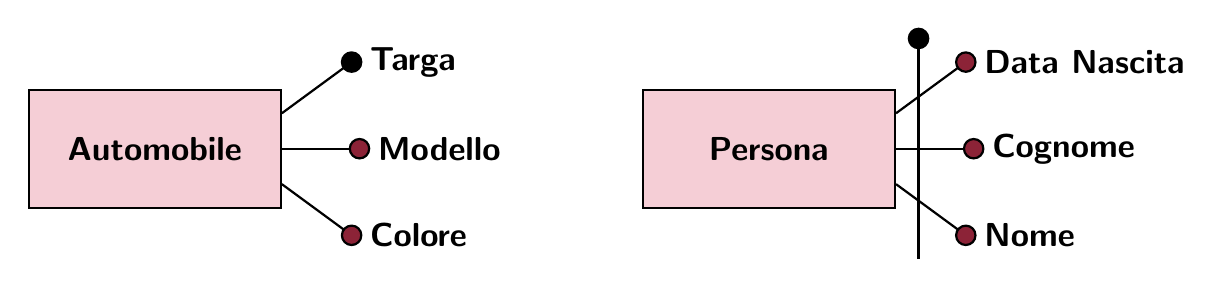
\begin{tikzpicture}[thick]
			\definecolor{softpink}{RGB}{245, 206, 214}
			\definecolor{darkred}{RGB}{140, 35, 55}
			
			% Entità: Automobile e Persona (affiancate sulla stessa riga orizzontale)
			\node[draw, fill=softpink, minimum width=3.2cm, minimum height=1.5cm, font=\sffamily\bfseries\large] (auto) at (0, 0) {Automobile};
			\node[draw, fill=softpink, minimum width=3.2cm, minimum height=1.5cm, font=\sffamily\bfseries\large] (pers) at (7.8, 0) {Persona};
			
			% Punti per gli attributi di Automobile
			\coordinate (pTarga)   at (2.5, 1.1);
			\coordinate (pModello) at (2.6, 0);
			\coordinate (pColore)  at (2.5, -1.1);
			
			% Linee per gli attributi di Automobile
			\draw (auto.east |- 0, 0.45) -- (pTarga);
			\draw (auto.east) -- (pModello);
			\draw (auto.east |- 0, -0.45) -- (pColore);
			
			% Pallini e testi degli attributi di Automobile (Targa con pallino nero identificatore)
			\filldraw[fill=black] (pTarga) circle (3.5pt) node[anchor=west, xshift=3pt, font=\sffamily\bfseries\large] {Targa};
			\filldraw[fill=darkred] (pModello) circle (3.5pt) node[anchor=west, xshift=3pt, font=\sffamily\bfseries\large] {Modello};
			\filldraw[fill=darkred] (pColore) circle (3.5pt) node[anchor=west, xshift=3pt, font=\sffamily\bfseries\large] {Colore};
			
			% Punti per gli attributi di Persona
			\coordinate (pData) at (10.3, 1.1);
			\coordinate (pCogn) at (10.4, 0);
			\coordinate (pNome) at (10.3, -1.1);
			
			% Linee per gli attributi di Persona
			\draw (pers.east |- 0, 0.45) -- (pData);
			\draw (pers.east) -- (pCogn);
			\draw (pers.east |- 0, -0.45) -- (pNome);
			
			% Barra verticale dell'identificatore composto di Persona
			\draw[thick] (9.7, -1.4) -- (9.7, 1.4);
			\filldraw[fill=black] (9.7, 1.4) circle (3.5pt);
			
			% Pallini e testi degli attributi di Persona
			\filldraw[fill=darkred] (pData) circle (3.5pt) node[anchor=west, xshift=3pt, font=\sffamily\bfseries\large] {Data Nascita};
			\filldraw[fill=darkred] (pCogn) circle (3.5pt) node[anchor=west, xshift=3pt, font=\sffamily\bfseries\large] {Cognome};
			\filldraw[fill=darkred] (pNome) circle (3.5pt) node[anchor=west, xshift=3pt, font=\sffamily\bfseries\large] {Nome};
		\end{tikzpicture}
		\caption{Esempio di identificatori interni semplici e composti.}
		\label{fig:identificatori_semplice_composto}
	\end{figure}
	
	\begin{osservazione}{Natura degli identificatori}{}
		\begin{itemize}
			\item Un entità deve avere \textbf{almeno} un identificatore, ma può averne anche più di uno.
			
			\item Un identificatore esterno è possibile solo per entità che partecipano ad un'associazione con cardinalità (1, 1).
			
			\item Per le associazioni non occorre un identificatore in quanto non rappresentano un fatto bensì un legame logico.
		\end{itemize}
	\end{osservazione}
	
	\subsection{Generalizzazioni}
	\begin{definizione}{Generalizzazione}{}
		Una generalizzazione è un costrutto che mette in relazione una o più entità $E_1, E_2, \dots, E_n$ con un'entità $E$ che le comprende come casi particolari. In poche parole, le entità $E_1,\dots, E_n$ sono delle sottoclassi (o \textbf{specializzazioni}) dell'entità $E$, e dunque ereditano tutte le caratteristiche dell'entità padre potendo poi definirne di nuove.
	\end{definizione}
	
	\begin{figure}[htbp]
		\centering
		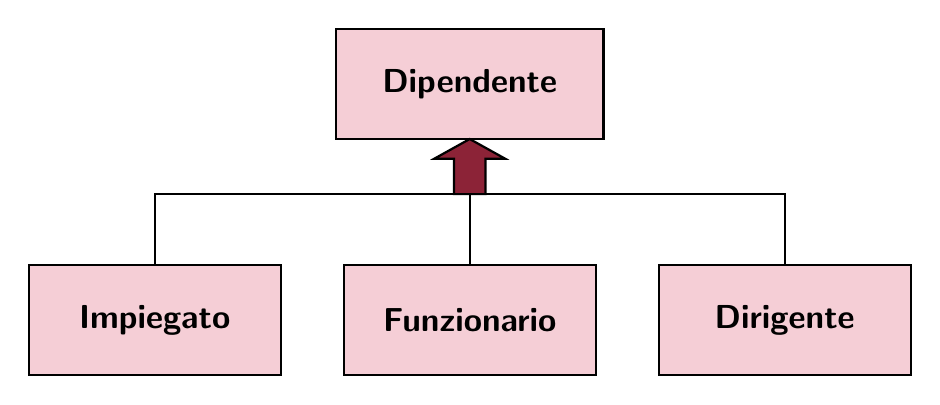
\begin{tikzpicture}[thick]
			\definecolor{softpink}{RGB}{245, 206, 214}
			\definecolor{darkred}{RGB}{140, 35, 55}
			
			% Entità genitore: Dipendente
			\node[draw, fill=softpink, minimum width=3.4cm, minimum height=1.4cm, font=\sffamily\bfseries\large] (dip) at (0, 3) {Dipendente};
			
			% Entità figlie: Impiegato, Funzionario e Dirigente
			\node[draw, fill=softpink, minimum width=3.2cm, minimum height=1.4cm, font=\sffamily\bfseries\large] (imp) at (-4, 0) {Impiegato};
			\node[draw, fill=softpink, minimum width=3.2cm, minimum height=1.4cm, font=\sffamily\bfseries\large] (funz) at (0, 0) {Funzionario};
			\node[draw, fill=softpink, minimum width=3.2cm, minimum height=1.4cm, font=\sffamily\bfseries\large] (dir) at (4, 0) {Dirigente};
			
			% Freccia spessa di generalizzazione rivolta verso l'entità genitore
			\draw[fill=darkred, draw=black] (-0.2, 1.6) -- (-0.2, 2.05) -- (-0.45, 2.05) -- (0, 2.3) -- (0.45, 2.05) -- (0.2, 2.05) -- (0.2, 1.6) -- cycle;
			
			% Linee di collegamento orizzontali e verticali dalle figlie alla freccia
			\draw (imp.north) -- (-4, 1.6) -- (4, 1.6) -- (dir.north);
			\draw (funz.north) -- (0, 1.6);
		\end{tikzpicture}
		\caption{Gerarchia di generalizzazione.}
		\label{fig:gerarchia_generalizzazione_dipendente}
	\end{figure}
	
	Una generalizzazione può essere
	\begin{description}
		\item [Totale:] quando ogni occorrenza dell'entità padre appartiene ad almeno un'occorrenza di una delle specializzazioni (in parole povere, quando un istanza del padre è del tipo di almeno un figlio). Un esempio potrebbe essere, \texttt{Persona <- Maggiorenne, Minorenne}. In questo caso è totale in quanto una persona è maggiorenne oppure minorenne.
		
		\item[Parziale:] quando esiste almeno un'occorrenza dell'entità padre che non appartiene ad alcuna categoria. Ad esempio \texttt{Animale <- Cane, Gatto}. Ovviamente cani e gatti non sono gli unici animali esistenti.
		
		\item[Esclusiva:] quando ogni occorrenza del padre può appartenere al massimo ad una categoria. Vale l'esempio di prima dei maggiorenni e minorenni.
		
		\item[Sovrapposta:] quando esiste almeno un'istanza dell'entità padre che appartiene a più categorie contemporaneamente. Un esempio in questo caso potrebbe essere \texttt{Persona <- Studente, Lavoratore}, in quanto una persona può contemporaneamente essere uno studente ma anche un lavoratore.
	\end{description}
	
	Concluso il discorso sui costrutti che riguardano il modello E-R, spendiamo due parole anche per parlare della documentazione da associare quando si sviluppa un modello concettuale.
	
	\begin{description}
		\item [Dizionario delle entità:] consiste in una tabella in cui si riportano le entità descritte nel modello assieme ad alcune informazioni importanti riguardanti queste: \textbf{nome, breve descrizione, attributi, identificatore univoco}.
		
		\item[Dizionario delle associazioni:] come quello delle entità, si tratta di una tabella volta a descrivere tutte le associazioni presenti nel modello. Si includono informazioni come: \textbf{nome, breve descrizione, entità coinvolte, attributi dell'associazione}.
		
		\item[Vincoli non esprimibili:] il modello concettuale è un ottimo strumento per rappresentare la realtà di riferimento del problema, tuttavia non è abbastanza esaustivo per quanto riguarda eventuali vincoli stabiliti sulla base di dati. Nell'ottica di una base di dati aziendale si potrebbe, ad esempio, impedire che un dirigente abbia uno stipendio inferiore a quello di un impiegato normale (ci rendiamo conto che è impossibile esprimere tale vincolo sul modello E-R). 
	\end{description}
	
	\chapter{Progettazione logica}
	Come seconda fase nella progettazione di una base di dati abbiamo la progettazione logica, in cui ci avviciniamo maggiormente all'architettura del DBMS e per questo bisogna definire il modello con cui si voglio opportunamente memorizzare i dati.\\
	In questo corso faremo esclusivamente uso del modello relazionale, che a breve vedremo con maggior dettaglio.
	
	\section{Il modello relazionale}
	Il modello relazionale si basa sul concetto matematico di \textbf{relazione}: tali relazioni si traducono in maniera naturale in tabelle (infatti talvolta i due termini potrebbero essere scambiati).
	Prima di passare alla definizione formale di questo modello, vediamo alcune definizioni di oggetti matematici che ci serviranno:
	
	\begin{definizione}{Dominio}{}
		Un \textbf{dominio} è un insieme potenzialmente infinito di valori. Ricordando lo studio di una funzione, il dominio di questa era l'insieme dei valori $x\in \mathbb{R}$ a cui la funzione associava un valore.
		\smallbreak
		Possiamo scegliere anche esempi più comuni di dominio: l'insieme dei numeri naturali, l'insieme dei valori in un sistema di numerazione binario (banalmente solo 0 e 1), l'insieme delle stringhe lunghe 20 caratteri, ...
	\end{definizione}
	
	\begin{definizione}{Prodotto cartesiano}{}
		Siano $D_1, D_2, \dots, D_k$ domini non necessariamente distinti. Il \textbf{prodotto cartesiano} tra tali domini è denotato come
		\[
			D_1 \times D_2 \times \dots \times D_k
		\]
		che, insiemisticamente, può essere visto come quella sequenza ordinata di valori in cui ogni valore è preso da un dominio diverso.
		\[
			\{(v_1, v_2, \dots, v_k) | v_1 \in D_1, v_2 \in D_2, \dots, v_k \in D_k\}
		\]
	\end{definizione}
	
	\begin{definizione}{Relazione matematica}{}
		Una \textbf{relazione}, in matematica, è un qualsiasi \textbf{sottoinsieme del prodotto cartesiano di uno o più domini}.
		\smallbreak
		
		Il \textbf{grado di una relazione} è il numero di domini coinvolti nel prodotto cartesiano che hanno prodotto quella relazione (dunque se abbiamo il prodotto cartesiano tra 5 domini e prendiamo una relazione su quel prodotto, il suo grado sarà 5).
		\smallbreak
		
		Gli elementi di una relazione sono detti \textbf{tuple} o \textbf{n-uple}, e il numero di n-uple di una relazione rappresenta la sua \textbf{cardinalità}.
		
		L'ordine fra gli elementi di una tupla (che sono presi ognuno da ogni dominio, in modo \textbf{ordinato}) è \textbf{importante}, mentre è irrilevante l'ordine delle tuple di una relazione (essendo essa un insieme).	
	\end{definizione}
	Supponiamo di avere due domini: $D_1 = \{\text{bianco, nero}\}, D_2 = \{1, 2, 3\}$.\\
	Il prodotto cartesiano sarà
	\[
		D_1 \times D_2 = \{\text{(bianco, 1), (bianco, 2), (bianco, 3), (nero, 1), (nero, 2), (nero, 3)}\}
	\]
	Presa una relazione $R = \{\text{(bianco, 1), (nero, 1), (nero, 3)}\}$, questa avrà grado 2 (in quanto è stata generata dal prodotto cartesiano di 2 domini) e cardinalità 3 (in quanto ha 3 elementi).
	
	Forniamo adesso dell'altra notazione riguardante relazioni e tuple.
	Sia $R$ una relazione di grado $k$. Sia $t \in R$. Sia $i \in \{1, \dots, k\}$. Denotiamo con $t[i]$ oppure $t.i$ l'\textbf{i-esima componente di t}.
	Per l'esempio di prima, supponiamo $t = \{(\text{nero}, 1)\}$. Abbiamo che t[1] = nero, t[2] = 1, t[1,2] = (nero, 1).
	
	Abbiamo già detto che nei database relazionali c'è una fortissima corrispondenza tra il concetto di tabella e quello di relazione. Il problema è che se ci viene data una tabella così senza descrizioni, decifrarne il contenuto diventa quasi impossibile.
	
	E' per questo che nasce l'importanza di definire degli attributi nelle tabelle.
	\begin{definizione}{Attributo}{}
		Un \textbf{attributo} è definito da un \textbf{nome} \texttt{A} e dal \textbf{dominio} di tutti i valori che \texttt{A} può assumere.
	\end{definizione}
	
	\begin{definizione}{Schema di relazione e tuple}{}
		\begin{itemize}
			\item Sia \texttt{R} un insieme di attributi diversi (\textbf{schema di relazione}, sarebbe l'intestazione della tabella). Una n-upla su \texttt{R} è una \textbf{funzione che associa ad ogni attributo A in R un elemento del dominio di A}.\\
			In poche parole, una n-upla, quella che informalmente chiameremmo \textit{riga della tabella} o \textit{istanza della tabella} viene matematicamente definita come una funzione che ad ogni colonna associa il suo effettivo valore, preso appunto dal dominio di valori consentiti dall'attributo.
			
			\item Se \texttt{t} è una n-upla su \texttt{R} ed \texttt{A} è un attributo di \texttt{R}, indichiamo con \texttt{t(A)} il valore assunto dalla funzione \texttt{t} in corrispondenza dell'attributo \texttt{A}.\\
			Sempre in parole molto povere, facendo \texttt{t(A)} ci viene restituito il valore che l'attributo \texttt{A} assume nella riga \texttt{t}.
			
			\item Se $Y \subseteq X$, dove X è lo schema di una relazione R, denotiamo con t[Y] l'insieme dei valori assunti dagli attributi $y \in Y$ nella tupla t.
		\end{itemize}		
	\end{definizione}
	
	Infine, possiamo definire lo \textbf{schema di una base di dati relazionale} come l'insieme di tutti gli schemi di relazione che hanno nomi differenti.
	\begin{tabella}[Dati relativi a città, regione di appartenenza e popolazione]{|X|X|X|}
		\hline
		\textbf{Città} & \textbf{Regione} & \textbf{Popolazione} \\
		\hline
		Roma    & Lazio     & 3000000 \\
		\hline
		Milano  & Lombardia & 1500000 \\
		\hline
		Genova  & Liguria   & 800000  \\
		\hline
		Pisa    & Toscana   & 150000  \\
	\end{tabella}
	
	\subsection{Chiavi di una relazione}
	Abbiamo già implicitamente parlato di chiavi quando, nel modello concettuale, citavamo gli identificatori di un'entità. Avendo però ora definito più concetti, possiamo fornire una definizione leggermente più formale di chiave.
	\begin{definizione}{Chiave}{}
		Una \textbf{chiave} è un attributo o un insieme di attributi che identifica univocamente una tupla.
		\smallbreak
		Supponendo che \texttt{X} sia un insieme di attributi che formano una chiave, valgono le seguenti proprietà:
		\begin{itemize}
			\item Se $t_1, t_2, t_1 \neq t_2$ tuple di una relazione R, allora $t_1[X] \neq t_2[X]$.
			
			\item $X$ è il più piccolo insieme che soddisfa la proprietà precedente.
		\end{itemize}
	\end{definizione}
	La chiave composta dal minor numero di attributi possibili ad identificare una tupla si dice \textbf{chiave primaria}.
	Questa gode di due fondamentali proprietà:
	\begin{itemize}
		\item Non può avere valori nulli.
		
		\item Consente di mettere in relazione tabelle diverse.
	\end{itemize}
	
	\section{Ristrutturazione del modello concettuale}
	Come mai la fase di ristrutturazione del modello concettuale appartiene alla progettazione logica?\\
	Ricordando quando detto nei primi capitoli, è molto importante progettare una base di dati mantenendo i paradigmi di indipendenza fisica e logica. Se nella prima fase di progettazione concettuale abbiamo descritto la realtà in modo completamente astratto e indipendente dalla memorizzazione fisica dei dati, con questa fase di ristrutturazione dovremo andare ad analizzare il modello concettuale già nell'ottica di voler organizzare i dati in tabelle e relazioni tra queste.
	Questo avviene in quanto l'obiettivo principale della progettazione logica è quello di \textbf{tradurre il modello concettuale in uno schema logico che rappresenti i dati nella stessa maniera}.
	\small
	Questa fase di ristrutturazione si articola in 4 attività principali.
	
	\subsection{Analisi delle ridondanze}
	Nello schema E-R, una ridondanza è la ripetizione di un'informazione utile ma derivabile da altre, ad esempio:
	\begin{itemize}
		\item Tramite operazioni di interrogazione sulla base di dati.
		
		\item Da altri attributi dell'entità stessa. Ad esempio, non ha senso inserire gli attributi \texttt{IVA, PrezzoNetto, PrezzoLordo} in un'entità \texttt{Prodotto}, in quanto questi attributi sono calcolabili a partire da almeno due di loro.
		
		\item Ridondanza derivata da più associazioni sulle stesse entità, ma \textbf{solo se le istanze delle associazioni rappresentano lo stesso risultato}.
	\end{itemize}
	
	\subsection{Eliminazione delle generalizzazioni}
	Il modello relazionale abbiamo visto essere in grado di rappresentare solo tabelle, non costrutti di ereditarietà come classi e oggetti. Per questo motivo è necessario eliminare tutte le gerarchie rappresentate nel modello concettuale, e ciò può essere fatto in 3 modi differenti:
	\begin{enumerate}
		\item \textbf{Accorpamento delle figlie nel padre (Roll-up)}
		\begin{itemize}
			\item \textbf{Cosa si fa:} Si elimina ogni entità figlia. L'entità padre assorbe tutti gli attributi specifici delle entità figlie e tutte le relazioni a cui partecipavano. Viene inoltre introdotto un apposito attributo \textit{selettore} (discriminatore di tipo), ad esempio \texttt{TipoPersona = \{'Studente', 'Docente'\}}, per identificare a quale sottocategoria appartiene ciascuna istanza.
			\item \textbf{Vantaggi:}
			\begin{itemize}
				\item Estrema semplicità nella gestione delle proprietà e operazioni comuni.
			\end{itemize}
			\item \textbf{Svantaggi:}
			\begin{itemize}
				\item Introduzione di valori nulli (\texttt{NULL}): se un'istanza è uno studente, tutti gli attributi propri del docente assumeranno valore nullo.
				\item Potenziale spreco di spazio su memoria secondaria e degradazione dell'integrità dei vincoli a livello di colonna.
			\end{itemize}
			\item \textbf{Condizioni e casi d'uso:} 
			Sempre applicabile senza vincoli di tipo di gerarchia. È la scelta ideale quando le entità figlie possiedono \textbf{pochi attributi specifici} e \textbf{poche relazioni proprie}, e la maggior parte delle operazioni coinvolge l'insieme complessivo delle istanze (padre e figlie insieme).
		\end{itemize}
		
		\item \textbf{Accorpamento del padre nelle figlie (Roll-down)}
		\begin{itemize}
			\item \textbf{Cosa si fa:} Si elimina l'entità padre e si mantengono unicamente le entità figlie. Ciascuna entità figlia eredita tutti gli attributi della classe padre (inclusa la chiave primaria) e tutte le relazioni a cui il padre prendeva parte.
			\item \textbf{Vantaggi:}
			\begin{itemize}
				\item Assenza totale di valori nulli dovuti alla gerarchia: ogni relazione contiene unicamente attributi significativi per le sue istanze.
				\item Accessi veloci e selettivi per tutte le operazioni mirate a una singola categoria figlia.
			\end{itemize}
			\item \textbf{Svantaggi:}
			\begin{itemize}
				\item Ridondanza concettuale: gli attributi e le relazioni originarie del padre vengono replicati nelle specifiche di ogni singola figlia.
			\end{itemize}
			\item \textbf{Condizioni e casi d'uso:} 
			Questo metodo è applicabile in modo naturale \textbf{solo se la generalizzazione è TOTALE}. Se fosse parziale, esisterebbero istanze del padre non appartenenti ad alcuna figlia, le quali andrebbero irrimediabilmente perdute eliminando l'entità radice. È inoltre altamente raccomandato che sia \textbf{esclusiva} (disgiunta), per evitare di duplicare la stessa entità in più tabelle figlie. Si predilige quando le entità figlie hanno molti attributi distinti e le interrogazioni avvengono quasi sempre separatamente su ciascuna figlia.
		\end{itemize}
		
		\item \textbf{Sostituzione della generalizzazione con associazioni}
		\begin{itemize}
			\item \textbf{Cosa si fa:} Si mantengono separate sia l'entità padre sia le entità figlie. La gerarchia viene rimpiazzata da associazioni binarie uno a uno (1:1) tra il padre e ciascuna entità figlia. Ogni tabella figlia adotta come chiave primaria la stessa chiave del padre, fungendo contemporaneamente da chiave esterna verso quest'ultimo.
			\item \textbf{Vantaggi:}
			\begin{itemize}
				\item Massima flessibilità e generalità: è sempre applicabile, indipendentemente dal fatto che la gerarchia sia totale/parziale o esclusiva/sovrapposta.
				\item Rispetto rigoroso della semantica originale, assenza di campi nulli anomali e nessuna duplicazione di tuple.
			\end{itemize}
			\item \textbf{Svantaggi:}
			\begin{itemize}
				\item Impatto sulle prestazioni: per ricostruire l'insieme completo delle informazioni di un'istanza figlia è sempre necessaria una complessa operazione di congiunzione tra le informazioni del padre e quelle della singola classe.
			\end{itemize}
			\item \textbf{Condizioni e casi d'uso:} 
			Sempre applicabile. È la soluzione di riferimento in caso di generalizzazioni \textbf{parziali} e/o \textbf{sovrapposte}, oppure quando sia l'entità genitore che quelle figlie dispongono di numerosi attributi e relazioni distinti e sussistono accessi eterogenei (sia generalisti che mirati alle sottoclassi).
		\end{itemize}
	\end{enumerate}
	
	\subsection{Partizionamento/accorpamento di entità e associazioni}
	Si tratta forse dell'operazione più ambigua, in quanto non dipende tanto dall'astrazione che abbiamo fatto del problema, bensì di come devono essere acceduti i dati dall'applicazione.
	Questa fase può svolgersi secondo 4 diverse modalità a seconda del caso.
	
	\begin{enumerate}
		\item \textbf{Partizionamento verticale di entità}: supponiamo di avere un'entità \texttt{Impiegato}, che contiene sia i dati anagrafici che lavorativi. Supponiamo anche che la nostra applicazione debba accedere separatamente ai dati lavorativi e quelli anagrafici. In questo caso potremmo pensare di suddividere l'entità \texttt{Impiegato(codice, cognome, indirizzo, data\_nascita, livello, stipendio, ritenute)} in due entità separate \texttt{DatiAnagrafici(codice, cognome, indirizzo, data\_nascita), DatiLavorativi(stipendio, livello, ritenute)}. In seguito queste due entità verranno collegate da un'apposita associazione che le mette in relazione in quanto fanno riferimento allo stesso impiegato.
		\begin{center}
			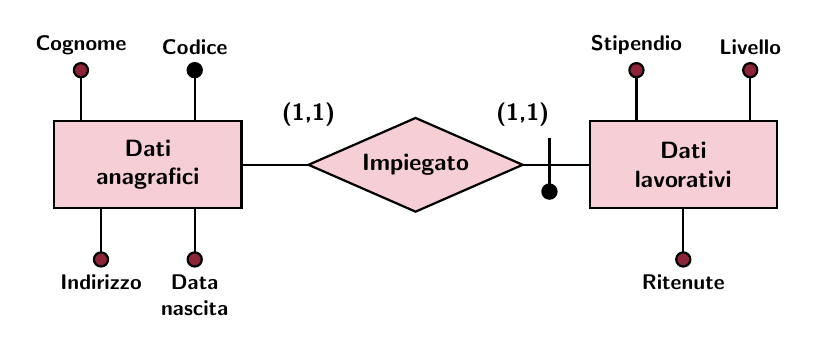
\begin{tikzpicture}[thick, scale=0.85, every node/.style={transform shape}]
				\definecolor{softpink}{RGB}{245, 206, 214}
				\definecolor{darkred}{RGB}{140, 35, 55}
				
				\def\rx{1.6}
				\def\ry{0.7}
				
				% Entità: Dati anagrafici e Dati lavorativi
				\node[draw, fill=softpink, minimum width=2.8cm, minimum height=1.3cm, font=\sffamily\bfseries\normalsize, align=center] (anag) at (0, 0) {Dati\\anagrafici};
				\node[draw, fill=softpink, minimum width=2.8cm, minimum height=1.3cm, font=\sffamily\bfseries\normalsize, align=center] (lav)  at (8.0, 0) {Dati\\lavorativi};
				
				% Relazione: Impiegato
				\coordinate (cImp) at (4.0, 0);
				\draw[fill=softpink] (cImp) ++(0, \ry) -- ++(\rx, -\ry) -- ++(-\rx, -\ry) -- ++(-\rx, \ry) -- cycle;
				\node[font=\sffamily\bfseries\normalsize] at (cImp) {Impiegato};
				
				% Linee di collegamento tra entità e relazione
				\draw (anag.east) -- ([xshift=-\rx cm]cImp);
				\draw ([xshift=\rx cm]cImp) -- (lav.west);
				
				% Cardinalità distanziate verticalmente dal rombo
				\node[font=\sffamily\bfseries\normalsize] at (2.4, 0.75) {(1,1)};
				\node[font=\sffamily\bfseries\normalsize] at (5.6, 0.75) {(1,1)};
				
				% Identificatore esterno su Dati lavorativi
				\draw[thick] (6.0, -0.4) -- (6.0, 0.4);
				\filldraw[fill=black] (6.0, -0.4) circle (3pt);
				
				% Attributi di Dati anagrafici
				\draw ([xshift=-1cm]anag.north) -- ++(0, 0.75) coordinate (aCognome);
				\filldraw[fill=darkred] (aCognome) circle (3pt) node[above=3pt, font=\sffamily\bfseries\small] {Cognome};
				
				\draw ([xshift=0.7cm]anag.north) -- ++(0, 0.75) coordinate (aCodice);
				\filldraw[fill=black] (aCodice) circle (3pt) node[above=3pt, font=\sffamily\bfseries\small] {Codice};
				
				\draw ([xshift=-0.7cm]anag.south) -- ++(0, -0.75) coordinate (aIndirizzo);
				\filldraw[fill=darkred] (aIndirizzo) circle (3pt) node[below=3pt, font=\sffamily\bfseries\small] {Indirizzo};
				
				\draw ([xshift=0.7cm]anag.south) -- ++(0, -0.75) coordinate (aDataNasc);
				\filldraw[fill=darkred] (aDataNasc) circle (3pt) node[below=3pt, font=\sffamily\bfseries\small, align=center] {Data\\nascita};
				
				% Attributi di Dati lavorativi
				\draw ([xshift=-0.7cm]lav.north) -- ++(0, 0.75) coordinate (aStipendio);
				\filldraw[fill=darkred] (aStipendio) circle (3pt) node[above=3pt, font=\sffamily\bfseries\small] {Stipendio};
				
				\draw ([xshift=1cm]lav.north) -- ++(0, 0.75) coordinate (aLivello);
				\filldraw[fill=darkred] (aLivello) circle (3pt) node[above=3pt, font=\sffamily\bfseries\small] {Livello};
				
				\draw (lav.south) -- ++(0, -0.75) coordinate (aRitenute);
				\filldraw[fill=darkred] (aRitenute) circle (3pt) node[below=3pt, font=\sffamily\bfseries\small] {Ritenute};
			\end{tikzpicture}
			\captionof{figure}{Esempio di partizionamento verticale}
			\label{fig:partizionamento_impiegato_compatto}
		\end{center}
		
		\item \textbf{Partizionamento orizzontale di associazioni}: supponiamo di avere una base di dati che mantiene le informazioni riguardo ai giocatori di una squadra da calcio, sia presenti che passati.
		\begin{center}
			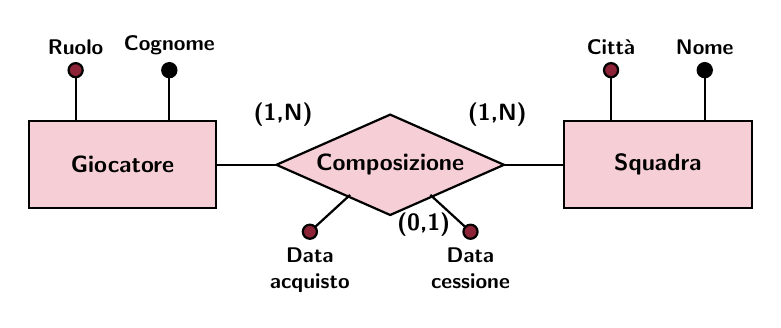
\begin{tikzpicture}[thick, scale=0.85, every node/.style={transform shape}]
				\definecolor{softpink}{RGB}{245, 206, 214}
				\definecolor{darkred}{RGB}{140, 35, 55}
				
				\def\rx{1.7}
				\def\ry{0.75}
				
				% Entità: Giocatore e Squadra
				\node[draw, fill=softpink, minimum width=2.8cm, minimum height=1.3cm, font=\sffamily\bfseries\normalsize] (gioc) at (0, 0) {Giocatore};
				\node[draw, fill=softpink, minimum width=2.8cm, minimum height=1.3cm, font=\sffamily\bfseries\normalsize] (squad) at (8.0, 0) {Squadra};
				
				% Relazione: Composizione
				\coordinate (cComp) at (4.0, 0);
				\draw[fill=softpink] (cComp) ++(0, \ry) -- ++(\rx, -\ry) -- ++(-\rx, -\ry) -- ++(-\rx, \ry) -- cycle;
				\node[font=\sffamily\bfseries\normalsize] at (cComp) {Composizione};
				
				% Linee di collegamento tra entità e relazione
				\draw (gioc.east) -- ([xshift=-\rx cm]cComp);
				\draw ([xshift=\rx cm]cComp) -- (squad.west);
				
				% Cardinalità distanziate verticalmente
				\node[font=\sffamily\bfseries\normalsize] at (2.4, 0.75) {(1,N)};
				\node[font=\sffamily\bfseries\normalsize] at (5.6, 0.75) {(1,N)};
				\node[font=\sffamily\bfseries\normalsize] at (4.5, -0.9) {(0,1)};
				
				% Attributi di Giocatore
				\draw ([xshift=-0.7cm]gioc.north) -- ++(0, 0.75) coordinate (aRuolo);
				\filldraw[fill=darkred] (aRuolo) circle (3pt) node[above=3pt, font=\sffamily\bfseries\small] {Ruolo};
				
				\draw ([xshift=0.7cm]gioc.north) -- ++(0, 0.75) coordinate (aCogn);
				\filldraw[fill=black] (aCogn) circle (3pt) node[above=3pt, font=\sffamily\bfseries\small] {Cognome};
				
				% Attributi di Squadra
				\draw ([xshift=-0.7cm]squad.north) -- ++(0, 0.75) coordinate (aCitta);
				\filldraw[fill=darkred] (aCitta) circle (3pt) node[above=3pt, font=\sffamily\bfseries\small] {Città};
				
				\draw ([xshift=0.7cm]squad.north) -- ++(0, 0.75) coordinate (aNomeS);
				\filldraw[fill=black] (aNomeS) circle (3pt) node[above=3pt, font=\sffamily\bfseries\small] {Nome};
				
				% Attributi della relazione Composizione
				\coordinate (pAcq) at (2.8, -1.0);
				\coordinate (pCes) at (5.2, -1.0);
				
				\draw ([xshift=-0.6cm, yshift=-0.45cm]cComp) -- (pAcq);
				\draw ([xshift=0.6cm, yshift=-0.45cm]cComp) -- (pCes);
				
				\filldraw[fill=darkred] (pAcq) circle (3pt) node[below=3pt, font=\sffamily\bfseries\small, align=center] {Data\\acquisto};
				\filldraw[fill=darkred] (pCes) circle (3pt) node[below=3pt, font=\sffamily\bfseries\small, align=center] {Data\\cessione};
			\end{tikzpicture}
			\label{fig:relazione_composizione_giocatore_squadra}
		\end{center}
		In un caso come questo, supponiamo ci sia richiesto di far accedere separatamente ai dati dei giocatori passati e di quelli correnti. Potremmo dividere dividere l'associazione \texttt{Composizione} in due associazioni tra \texttt{Composizione attuale} e \texttt{Composizione passata}, in modo da gestire separatamente i due casi.
		
		\begin{center}
			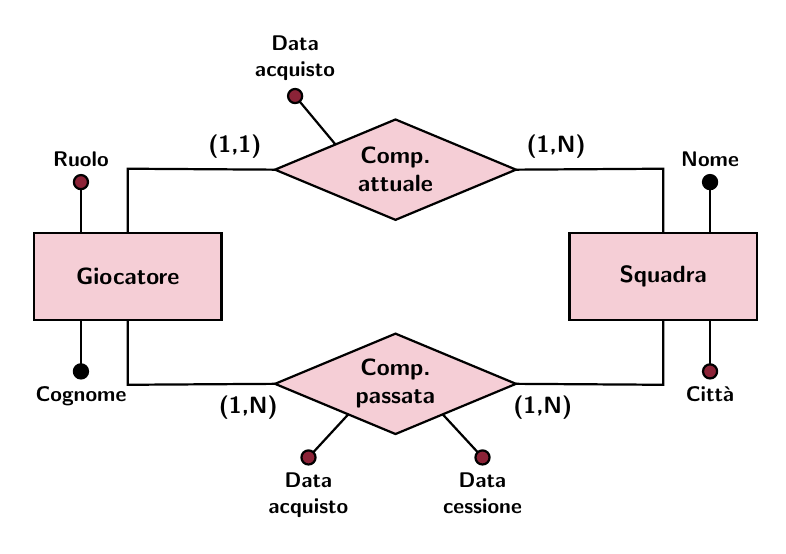
\begin{tikzpicture}[thick, scale=0.85, every node/.style={transform shape}]
				\definecolor{softpink}{RGB}{245, 206, 214}
				\definecolor{darkred}{RGB}{140, 35, 55}
				
				\def\rx{1.8}
				\def\ry{0.75}
				
				% Entità: Giocatore e Squadra
				\node[draw, fill=softpink, minimum width=2.8cm, minimum height=1.3cm, font=\sffamily\bfseries\normalsize] (gioc) at (0, 0) {Giocatore};
				\node[draw, fill=softpink, minimum width=2.8cm, minimum height=1.3cm, font=\sffamily\bfseries\normalsize] (squad) at (8.0, 0) {Squadra};
				
				% Relazione superiore: Comp. attuale
				\coordinate (cAtt) at (4.0, 1.6);
				\draw[fill=softpink] (cAtt) ++(0, \ry) -- ++(\rx, -\ry) -- ++(-\rx, -\ry) -- ++(-\rx, \ry) -- cycle;
				\node[font=\sffamily\bfseries\normalsize, align=center] at (cAtt) {Comp.\\attuale};
				
				% Relazione inferiore: Comp. passata
				\coordinate (cPas) at (4.0, -1.6);
				\draw[fill=softpink] (cPas) ++(0, \ry) -- ++(\rx, -\ry) -- ++(-\rx, -\ry) -- ++(-\rx, \ry) -- cycle;
				\node[font=\sffamily\bfseries\normalsize, align=center] at (cPas) {Comp.\\passata};
				
				% Linee di collegamento per la relazione superiore
				\draw (gioc.north) -- ++(0, 0.95) -- ([xshift=-\rx cm]cAtt);
				\draw (squad.north) -- ++(0, 0.95) -- ([xshift=\rx cm]cAtt);
				
				% Linee di collegamento per la relazione inferiore
				\draw (gioc.south) -- ++(0, -0.95) -- ([xshift=-\rx cm]cPas);
				\draw (squad.south) -- ++(0, -0.95) -- ([xshift=\rx cm]cPas);
				
				% Cardinalità separate e distanziate dalle linee
				\node[font=\sffamily\bfseries\normalsize] at (1.6, 1.95) {(1,1)};
				\node[font=\sffamily\bfseries\normalsize] at (6.4, 1.95) {(1,N)};
				\node[font=\sffamily\bfseries\normalsize] at (1.8, -1.95) {(1,N)};
				\node[font=\sffamily\bfseries\normalsize] at (6.2, -1.95) {(1,N)};
				
				% Attributi di Giocatore
				\draw ([xshift=-0.7cm]gioc.north) -- ++(0, 0.75) coordinate (aRuolo);
				\filldraw[fill=darkred] (aRuolo) circle (3pt) node[above=3pt, font=\sffamily\bfseries\small] {Ruolo};
				
				\draw ([xshift=-0.7cm]gioc.south) -- ++(0, -0.75) coordinate (aCognome);
				\filldraw[fill=black] (aCognome) circle (3pt) node[below=3pt, font=\sffamily\bfseries\small] {Cognome};
				
				% Attributi di Squadra
				\draw ([xshift=0.7cm]squad.north) -- ++(0, 0.75) coordinate (aNome);
				\filldraw[fill=black] (aNome) circle (3pt) node[above=3pt, font=\sffamily\bfseries\small] {Nome};
				
				\draw ([xshift=0.7cm]squad.south) -- ++(0, -0.75) coordinate (aCitta);
				\filldraw[fill=darkred] (aCitta) circle (3pt) node[below=3pt, font=\sffamily\bfseries\small] {Città};
				
				% Attributo di Comp. attuale
				\coordinate (pAcqAtt) at (2.5, 2.7);
				\draw ([xshift=-0.9cm, yshift=0.38cm]cAtt) -- (pAcqAtt);
				\filldraw[fill=darkred] (pAcqAtt) circle (3pt) node[above=3pt, font=\sffamily\bfseries\small, align=center] {Data\\acquisto};
				
				% Attributi di Comp. passata
				\coordinate (pAcqPas) at (2.7, -2.7);
				\coordinate (pCesPas) at (5.3, -2.7);
				
				\draw ([xshift=-0.7cm, yshift=-0.45cm]cPas) -- (pAcqPas);
				\draw ([xshift=0.7cm, yshift=-0.45cm]cPas) -- (pCesPas);
				
				\filldraw[fill=darkred] (pAcqPas) circle (3pt) node[below=3pt, font=\sffamily\bfseries\small, align=center] {Data\\acquisto};
				\filldraw[fill=darkred] (pCesPas) circle (3pt) node[below=3pt, font=\sffamily\bfseries\small, align=center] {Data\\cessione};
			\end{tikzpicture}
			\captionof{figure}{Partizionamento orizzontale di associazioni.}
			\label{fig:storicizzazione_composizione}
		\end{center}
		
		\item \textbf{Eliminazione di attributi multivalore}. Possiamo avere due istanze di attributi multivalore:
		\begin{itemize}
			\item Un attributo che ha cardinalità (0, N) oppure (1, N). In tal caso, l'attributo deve diventare un'entità a sé stante, associata all'entità di cui era attributo.
			\begin{center}
				\resizebox{\linewidth}{!}{%
					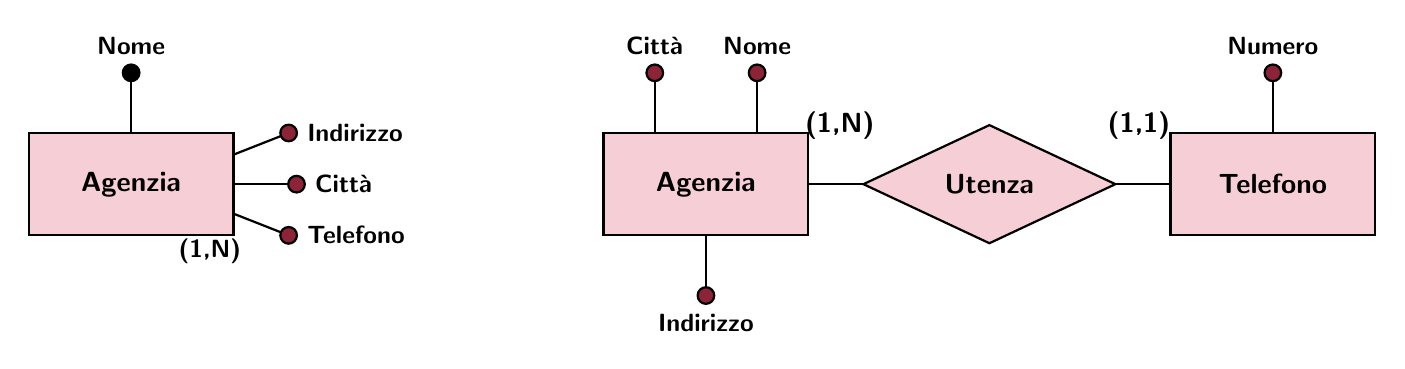
\begin{tikzpicture}[thick]
						\definecolor{softpink}{RGB}{245, 206, 214}
						\definecolor{darkred}{RGB}{140, 35, 55}
						
						\def\rx{1.6}
						\def\ry{0.75}
						
						% PARTE SINISTRA: Entità Agenzia con attributo multivalore
						
						% Entità Agenzia sinistra
						\node[draw, fill=softpink, minimum width=2.6cm, minimum height=1.3cm, font=\sffamily\bfseries\normalsize] (ag1) at (0, 0) {Agenzia};
						
						% Attributo identificatore: Nome
						\draw (ag1.north) -- ++(0, 0.75) coordinate (pNome1);
						\filldraw[fill=black] (pNome1) circle (3pt) node[above=3pt, font=\sffamily\bfseries\small] {Nome};
						
						% Attributi laterali: Indirizzo, Città e Telefono
						\coordinate (pInd1) at (2.0, 0.65);
						\coordinate (pCit1) at (2.1, 0);
						\coordinate (pTel1) at (2.0, -0.65);
						
						\draw (ag1.east |- 0, 0.38) -- (pInd1);
						\draw (ag1.east) -- (pCit1);
						\draw (ag1.east |- 0, -0.38) -- (pTel1);
						
						\filldraw[fill=darkred] (pInd1) circle (3pt) node[anchor=west, xshift=3pt, font=\sffamily\bfseries\small] {Indirizzo};
						\filldraw[fill=darkred] (pCit1) circle (3pt) node[anchor=west, xshift=3pt, font=\sffamily\bfseries\small] {Città};
						\filldraw[fill=darkred] (pTel1) circle (3pt) node[anchor=west, xshift=3pt, font=\sffamily\bfseries\small] {Telefono};
						
						% Cardinalità per l'attributo multivalore Telefono
						\node[font=\sffamily\bfseries\small] at (1.0, -0.85) {(1,N)};
						
						% PARTE DESTRA: Reificazione dell'attributo in entità Telefono e relazione Utenza
						
						% Entità Agenzia e Telefono
						\node[draw, fill=softpink, minimum width=2.6cm, minimum height=1.3cm, font=\sffamily\bfseries\normalsize] (ag2) at (7.3, 0) {Agenzia};
						\node[draw, fill=softpink, minimum width=2.6cm, minimum height=1.3cm, font=\sffamily\bfseries\normalsize] (tel2) at (14.5, 0) {Telefono};
						
						% Relazione: Utenza
						\coordinate (cUtenza) at (10.9, 0);
						\draw[fill=softpink] (cUtenza) ++(0, \ry) -- ++(\rx, -\ry) -- ++(-\rx, -\ry) -- ++(-\rx, \ry) -- cycle;
						\node[font=\sffamily\bfseries\normalsize] at (cUtenza) {Utenza};
						
						% Linee di collegamento tra entità e relazione
						\draw (ag2.east) -- ([xshift=-\rx cm]cUtenza);
						\draw ([xshift=\rx cm]cUtenza) -- (tel2.west);
						
						% Cardinalità separate e distanziate
						\node[font=\sffamily\bfseries\normalsize] at (9.0, 0.75) {(1,N)};
						\node[font=\sffamily\bfseries\normalsize] at (12.8, 0.75) {(1,1)};
						
						% Attributi dell'entità Agenzia destra
						\draw ([xshift=-0.65cm]ag2.north) -- ++(0, 0.75) coordinate (aCit2);
						\filldraw[fill=darkred] (aCit2) circle (3pt) node[above=3pt, font=\sffamily\bfseries\small] {Città};
						
						\draw ([xshift=0.65cm]ag2.north) -- ++(0, 0.75) coordinate (aNome2);
						\filldraw[fill=darkred] (aNome2) circle (3pt) node[above=3pt, font=\sffamily\bfseries\small] {Nome};
						
						\draw (ag2.south) -- ++(0, -0.75) coordinate (aInd2);
						\filldraw[fill=darkred] (aInd2) circle (3pt) node[below=3pt, font=\sffamily\bfseries\small] {Indirizzo};
						
						% Attributo dell'entità Telefono
						\draw (tel2.north) -- ++(0, 0.75) coordinate (aNum2);
						\filldraw[fill=darkred] (aNum2) circle (3pt) node[above=3pt, font=\sffamily\bfseries\small] {Numero};
					\end{tikzpicture}%
				}
			\end{center}
			
			\item In caso di un attributo che comprende più informazioni (come il precedente esempio di \texttt{Indirizzo = Via, Numero civico, CAP}), questo deve essere separato nei suoi attributi atomici.
			
		\end{itemize}
		
	\end{enumerate}
	
	\subsection{Scelta degli identificatori primari}
	Come abbiamo visto prima, la \textbf{chiave primaria} di un'entità è il più piccolo insieme di attributi che identifica in modo univoco ogni tupla. Guardando con occhio di riguardo anche la progettazione logica, possiamo aggiungere un paio di vincoli:
	\begin{itemize}
		\item Preferibilmente scegliere tra identificatori interno. Se non possibile, è consentito aggiungere un codice artificiale che identifichi la tupla.
		
		\item Deve essere un attributo che viene utilizzato nelle operazioni più frequenti ed importanti.
	\end{itemize}
	
	\section{La traduzione da schema concettuale a logico}
	Dopo aver rivisto e ristrutturato il modello concettuale con un occhio di riguardo per quella che sarà la rappresentazione dei dati secondo il modello logico, è arrivato il momento di capire come tradurre effettivamente i costrutti del modello concettuale in quelli del modello logico scelto (quello relazionale, nel nostro caso).
	
	\subsection{Le entità}
	Di una cosa siamo certi: le entità diventeranno le \textbf{tabelle} (o relazioni) del nostro modello logico. Ogni tabella dovrà anche preservare l'insieme degli attributi descritti dal modello concettuale.
	
	\subsection{Le associazioni}
	Per le associazioni, ovvero le effettive relazioni che vengono stabilite tra due o più schemi, il discorso è leggermente più delicato, in quanto non esiste un modo strettamente deterministico per rappresentarle.\\
	Prima di discutere separatamente ogni tipo di associazione che possiamo incontrare all'interno dello schema E-R e la rispettiva traduzione nel modello logico, dobbiamo introdurre un fondamentale concetto delle basi di dati relazionali.
	
	\begin{definizione}{Vincolo di integrità referenziale}{}
		Si tratta di uno dei tanti vincoli di integrità che si stabiliscono all'interno di una base di dati relazionale.\\
		In particolare, questo vincolo stabilisce un \textbf{collegamento logico tra due schemi attraverso uno o più attributi con dominio comune}.
		\smallbreak
		Parlando in modo più formale, supponiamo di avere una tabella $R_1$ con un insieme di attributi $X$. Prendiamo adesso un'altra tabella $R_2$.
		Stabilendo un vincolo di integrità referenziale fra le tabelle $R_1$ ed $R_2$ su $X$ significa \textbf{imporre} che i valori assunti da $X$ in $R_1$ debbano comparire come valori della chiave primaria di $R_2$. Tale insieme di attributi, nella tabella di "arrivo" $R_1$ viene detto \textbf{chiave esterna} o \textbf{foreign key}.
		\smallbreak
		In parole povere, stiamo dicendo che se in $R_1$ abbiamo un insieme di attributi $X$, affinché il vincolo di integrità referenziale con $R_2$ sia valido dobbiamo avere la certezza che $R_2$ contenga i valori di chiave primaria espressi da $X$ in almeno una n-upla.
	\end{definizione}
	
	Avendo definito il concetto di chiave esterna, possiamo procedere ad analizzare uno ad uno i tipi di associazione.
	
	\subsubsection{Associazioni: Molti a molti}
	Un'associazione \textit{molti a molti} si traduce come una vera e propria \textbf{tabella} che ha come chiave \textbf{l'insieme degli attributi chiave delle tabelle coinvolte nell'associazione}. Inoltre, tale tabella include anche eventuali attributi dell'associazione.
	\begin{figure}[htbp]
		\centering
		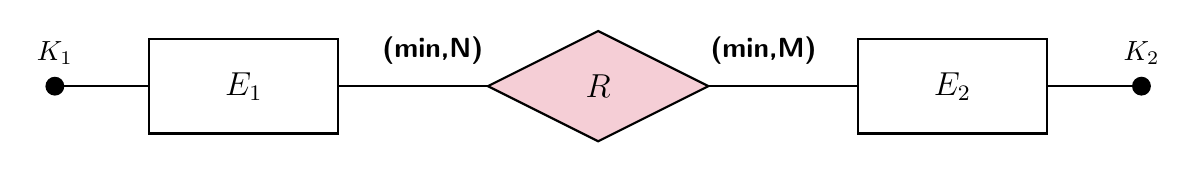
\begin{tikzpicture}[thick]
			\definecolor{softpink}{RGB}{245, 206, 214}
			
			\def\rx{1.4}
			\def\ry{0.7}
			
			% Entità E1 ed E2
			\node[draw, fill=white, minimum width=2.4cm, minimum height=1.2cm, font=\sffamily\bfseries\large] (e1) at (0, 0) {$E_1$};
			\node[draw, fill=white, minimum width=2.4cm, minimum height=1.2cm, font=\sffamily\bfseries\large] (e2) at (9.0, 0) {$E_2$};
			
			% Relazione R
			\coordinate (cR) at (4.5, 0);
			\draw[fill=softpink] (cR) ++(0, \ry) -- ++(\rx, -\ry) -- ++(-\rx, -\ry) -- ++(-\rx, \ry) -- cycle;
			\node[font=\sffamily\bfseries\large] at (cR) {$R$};
			
			% Linee di collegamento tra entità e relazione
			\draw (e1.east) -- ([xshift=-\rx cm]cR);
			\draw ([xshift=\rx cm]cR) -- (e2.west);
			
			% Cardinalità distanziate verticalmente dalle linee
			\node[font=\sffamily\bfseries\normalsize] at (2.4, 0.45) {(min,N)};
			\node[font=\sffamily\bfseries\normalsize] at (6.6, 0.45) {(min,M)};
			
			% Identificatore K1 di E1
			\draw (e1.west) -- (-2.4, 0);
			\filldraw[fill=black] (-2.4, 0) circle (3pt) node[above=4pt, font=\sffamily\bfseries\normalsize] {$K_1$};
			
			% Identificatore K2 di E2
			\draw (e2.east) -- (11.4, 0);
			\filldraw[fill=black] (11.4, 0) circle (3pt) node[above=4pt, font=\sffamily\bfseries\normalsize] {$K_2$};
		\end{tikzpicture}
		\caption{Modello concettuale generico di una associazione molti a molti.}
	\end{figure}
	
	Secondo quanto detto prima, il frammento di schema mostrato si traduce con le seguenti relazioni:
	\begin{center}
		E1(\textbf{K1}, attributi di E1...)\\
		E2(\textbf{K2}, attributi di E2...)\\
		R(\textbf{K1}, \textbf{K2}, attributi dell'associazione...)\\
	\end{center}
	E stabilendo anche i vincoli di integrità referenziale:
	\begin{itemize}
		\item Tra K1 in R e K1 in E1.
		\item Tra K2 in R e K2 in E2.
	\end{itemize}
	
	Generalmente, è consigliato rinominare gli attributi che costituiscono un vincolo di integrità referenziale, dando come nome un qualcosa di indicativo della tabella di provenienza (es: se l'attributo di partenza si chiama \texttt{Codice} e proviene dalla tabella \texttt{Impiegato}, potremmo chiamare la chiave esterna come \texttt{FK\_Codice\_Impiegato} oppure semplicemente \texttt{Impiegato}. In caso di chiavi composte da più attributi, possiamo rinominarle come \texttt{Impiegato1}, \texttt{Impiegato2}, ...). 
	
	Particolare attenzione deve essere posta sulle associazioni molti a molti ricorsive, in quanto in quel caso è di vitale importanza il nome delle chiavi esterne.
	\begin{figure}[htbp]
		\centering
		\resizebox{0.50\linewidth}{!}{
		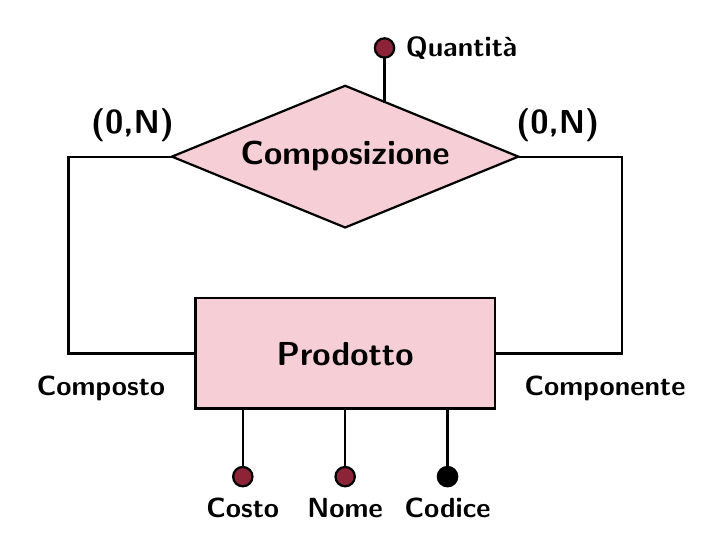
\begin{tikzpicture}[thick]
			\definecolor{softpink}{RGB}{245, 206, 214}
			\definecolor{darkred}{RGB}{140, 35, 55}
			
			\def\rx{2.2}
			\def\ry{0.9}
			
			% Entità: Prodotto
			\node[draw, fill=softpink, minimum width=3.8cm, minimum height=1.4cm, font=\sffamily\bfseries\large] (prod) at (0, 0) {Prodotto};
			
			% Relazione ricorsiva ingrandita: Composizione
			\coordinate (cComp) at (0, 2.5);
			\draw[fill=softpink] (cComp) ++(0, \ry) -- ++(\rx, -\ry) -- ++(-\rx, -\ry) -- ++(-\rx, \ry) -- cycle;
			\node[font=\sffamily\bfseries\large] at (cComp) {Composizione};
			
			% Linee dell'anello ricorsivo ampliate verso l'esterno
			\draw (prod.west) -- ++(-1.6, 0) -- ++(0, 2.5) -- ([xshift=-\rx cm]cComp);
			\draw (prod.east) -- ++(1.6, 0) -- ++(0, 2.5) -- ([xshift=\rx cm]cComp);
			
			% Ruoli ricorsivi distanziati orizzontalmente dal box di Prodotto
			\node[font=\sffamily\bfseries\normalsize] at (-3.1, -0.45) {Composto};
			\node[font=\sffamily\bfseries\normalsize] at (3.3, -0.45) {Componente};
			
			% Cardinalità distanziate verticalmente e orizzontalmente
			\node[font=\sffamily\bfseries\large] at (-2.7, 2.9) {(0,N)};
			\node[font=\sffamily\bfseries\large] at (2.7, 2.9) {(0,N)};
			
			% Attributo della relazione: Quantità
			\draw ([xshift=0.5cm, yshift=0.68cm]cComp) -- ++(0, 0.7) coordinate (aQuant);
			\filldraw[fill=darkred] (aQuant) circle (3.5pt) node[anchor=west, xshift=4pt, font=\sffamily\bfseries\normalsize] {Quantità};
			
			% Attributi di Prodotto maggiormente spaziati tra loro
			\draw ([xshift=-1.3cm]prod.south) -- ++(0, -0.85) coordinate (aCosto);
			\filldraw[fill=darkred] (aCosto) circle (3.5pt) node[below=4pt, font=\sffamily\bfseries\normalsize] {Costo};
			
			\draw (prod.south) -- ++(0, -0.85) coordinate (aNome);
			\filldraw[fill=darkred] (aNome) circle (3.5pt) node[below=4pt, font=\sffamily\bfseries\normalsize] {Nome};
			
			\draw ([xshift=1.3cm]prod.south) -- ++(0, -0.85) coordinate (aCodice);
			\filldraw[fill=black] (aCodice) circle (3.5pt) node[below=4pt, font=\sffamily\bfseries\normalsize] {Codice};
		\end{tikzpicture}
		}
		\caption{Esempio di associazione molti a molti ricorsiva.}
	\end{figure}
	
	La derivazione di questo modello concettuale sarà
	\begin{center}
		Prodotto(\textbf{Codice}, Nome, Costo)\\
		Composizione(\textbf{CodiceComposto}, \textbf{CodiceComponente}, Quantita)
	\end{center}
	In questo caso i due codici presenti nella tabella \texttt{Composizione} non saranno altro che codici di prodotti però inseriti come chiavi esterne.
	
	Un ultimo esempio sulle associazioni molti-a-molti per associazioni n-arie:
	\begin{figure}[htbp]
		\centering
		\resizebox{0.70\linewidth}{!}{
		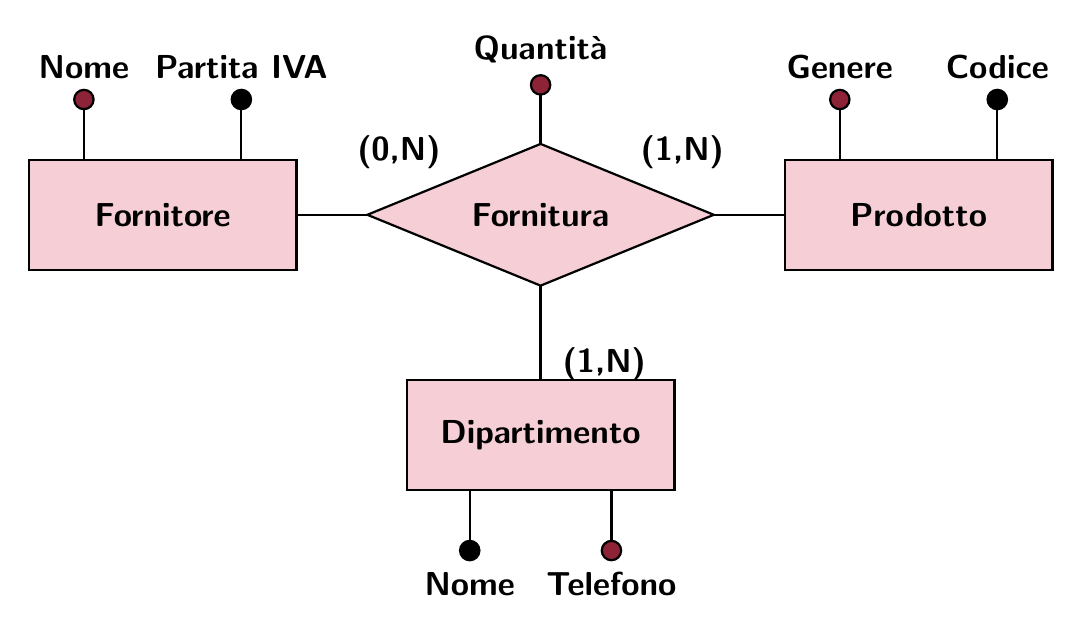
\begin{tikzpicture}[thick]
			\definecolor{softpink}{RGB}{245, 206, 214}
			\definecolor{darkred}{RGB}{140, 35, 55}
			
			\def\rx{2.2}
			\def\ry{0.9}
			
			% Coordinate centrali delle entità e della relazione ternaria
			\coordinate (cFornitura) at (4.8, 0);
			
			% Entità: Fornitore, Prodotto, Dipartimento
			\node[draw, fill=softpink, minimum width=3.4cm, minimum height=1.4cm, font=\sffamily\bfseries\large] (forn) at (0, 0) {Fornitore};
			\node[draw, fill=softpink, minimum width=3.4cm, minimum height=1.4cm, font=\sffamily\bfseries\large] (prod) at (9.6, 0) {Prodotto};
			\node[draw, fill=softpink, minimum width=3.4cm, minimum height=1.4cm, font=\sffamily\bfseries\large] (dip)  at (4.8, -2.8) {Dipartimento};
			
			% Relazione ternaria: Fornitura
			\draw[fill=softpink] (cFornitura) ++(0, \ry) -- ++(\rx, -\ry) -- ++(-\rx, -\ry) -- ++(-\rx, \ry) -- cycle;
			\node[font=\sffamily\bfseries\large] at (cFornitura) {Fornitura};
			
			% Linee di collegamento tra entità e relazione
			\draw (forn.east) -- ([xshift=-\rx cm]cFornitura);
			\draw ([xshift=\rx cm]cFornitura) -- (prod.west);
			\draw ([yshift=-\ry cm]cFornitura) -- (dip.north);
			
			% Cardinalità distanziate verticalmente e orizzontalmente dalle linee
			\node[font=\sffamily\bfseries\large] at (3.0, 0.8) {(0,N)};
			\node[font=\sffamily\bfseries\large] at (6.6, 0.8) {(1,N)};
			\node[font=\sffamily\bfseries\large, anchor=west] at (4.95, -1.9) {(1,N)};
			
			% Attributo della relazione: Quantità
			\draw ([yshift=\ry cm]cFornitura) -- ++(0, 0.75) coordinate (aQuant);
			\filldraw[fill=darkred] (aQuant) circle (3.5pt) node[above=4pt, font=\sffamily\bfseries\large] {Quantità};
			
			% Attributi di Fornitore
			\draw ([xshift=-1.0cm]forn.north) -- ++(0, 0.75) coordinate (aNomeF);
			\filldraw[fill=darkred] (aNomeF) circle (3.5pt) node[above=4pt, font=\sffamily\bfseries\large] {Nome};
			
			\draw ([xshift=1.0cm]forn.north) -- ++(0, 0.75) coordinate (aPiva);
			\filldraw[fill=black] (aPiva) circle (3.5pt) node[above=4pt, font=\sffamily\bfseries\large] {Partita IVA};
			
			% Attributi di Prodotto
			\draw ([xshift=-1.0cm]prod.north) -- ++(0, 0.75) coordinate (aGen);
			\filldraw[fill=darkred] (aGen) circle (3.5pt) node[above=4pt, font=\sffamily\bfseries\large] {Genere};
			
			\draw ([xshift=1.0cm]prod.north) -- ++(0, 0.75) coordinate (aCod);
			\filldraw[fill=black] (aCod) circle (3.5pt) node[above=4pt, font=\sffamily\bfseries\large] {Codice};
			
			% Attributi di Dipartimento
			\draw ([xshift=-0.9cm]dip.south) -- ++(0, -0.75) coordinate (aNomeD);
			\filldraw[fill=black] (aNomeD) circle (3.5pt) node[below=4pt, font=\sffamily\bfseries\large] {Nome};
			
			\draw ([xshift=0.9cm]dip.south) -- ++(0, -0.75) coordinate (aTel);
			\filldraw[fill=darkred] (aTel) circle (3.5pt) node[below=4pt, font=\sffamily\bfseries\large] {Telefono};
		\end{tikzpicture}
		}	
		\caption{Esempio di associazione n-aria molti-a-molti.}
	\end{figure}
	
	In questo caso si deriva come ci si aspetterebbe, ma si è scelto di mostrare un esempio per evitare che il lettore si cogliesse impreparato. Il fulcro è sempre creare una tabella per l'associazione e mettere al suo interno aventuali attributi dell'associazione e, come chiave primaria, l'insieme delle chiavi di ogni tabella coinvolta.\\
	La derivazione risulta dunque:
	\begin{center}
		Fornitore(\textbf{PartitaIVA}, Nome)\\
		Prodotto(\textbf{Codice}, Genere)\\
		Dipartimento(\textbf{Nome}, Telefono)\\
		Fornitura(\textbf{Fornitore}, \textbf{Prodotto}, \textbf{Dipartimento}, Quantita)
	\end{center}
	
	\subsubsection{Associazioni: Uno a molti}
	Per questo tipo di associazioni, si può procedere in due modalità diverse:
	\begin{enumerate}
		\item \textbf{Creare una tabella per l'associazione}, al cui interno si metterà:
		\begin{itemize}
			\item Come \textbf{chiave primaria}, la \textbf{chiave primaria della tabella che partecipa all'associazione con cardinalità (min,1)} (che sarà anche chiave esterna, legata da vincolo di integrità referenziale).
			\item Come \textbf{chiave esterna}, la \textbf{chiave primaria della tabella che partecipa all'associazione con cardinalità (min,N)}.
		\end{itemize}
		
		\item \textbf{Inserire nella tabella che partecipa con cardinalità (min,1) un vincolo di integrità referenziale alla chiave primaria della tabella che partecipa con (min, N)}. Tutti gli eventuali attributi dell'associazione andranno a finire nella tabella con cardinalità (min,1).
	\end{enumerate}
	
	Vediamo di seguito un esempio di modello concettuale, e discutiamo le due possibili traduzioni nel modello logico.
	\begin{figure}[htbp]
		\centering
		\resizebox{0.70\linewidth}{!}{%
			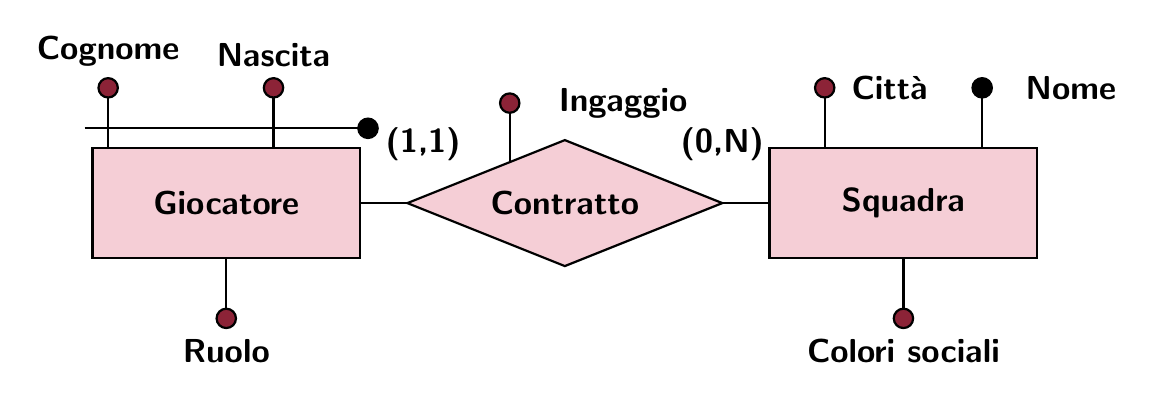
\begin{tikzpicture}[thick]
				\definecolor{softpink}{RGB}{245, 206, 214}
				\definecolor{darkred}{RGB}{140, 35, 55}
				
				\def\rx{2.0}
				\def\ry{0.8}
				
				% Entità: Giocatore e Squadra
				\node[draw, fill=softpink, minimum width=3.4cm, minimum height=1.4cm, font=\sffamily\bfseries\large] (gioc) at (0, 0) {Giocatore};
				\node[draw, fill=softpink, minimum width=3.4cm, minimum height=1.4cm, font=\sffamily\bfseries\large] (squad) at (8.6, 0) {Squadra};
				
				% Relazione: Contratto
				\coordinate (cContr) at (4.3, 0);
				\draw[fill=softpink] (cContr) ++(0, \ry) -- ++(\rx, -\ry) -- ++(-\rx, -\ry) -- ++(-\rx, \ry) -- cycle;
				\node[font=\sffamily\bfseries\large] at (cContr) {Contratto};
				
				% Linee di collegamento tra entità e relazione
				\draw (gioc.east) -- ([xshift=-\rx cm]cContr);
				\draw ([xshift=\rx cm]cContr) -- (squad.west);
				
				% Cardinalità distanziate e posizionate in modo indipendente
				\node[font=\sffamily\bfseries\large] at (2.5, 0.75) {(1,1)};
				\node[font=\sffamily\bfseries\large] at (6.3, 0.75) {(0,N)};
				
				% Attributo della relazione: Ingaggio
				\draw ([xshift=-0.7cm, yshift=0.52cm]cContr) -- ++(0, 0.75) coordinate (aIngaggio);
				\filldraw[fill=darkred] (aIngaggio) circle (3.5pt) node[anchor=west, xshift=14pt, font=\sffamily\bfseries\large] {Ingaggio};
				
				% Attributi dell'entità Giocatore
				\draw ([xshift=-1.5cm]gioc.north) -- ++(0, 0.75) coordinate (aCogn);
				\filldraw[fill=darkred] (aCogn) circle (3.5pt) node[above=4pt, font=\sffamily\bfseries\large] {Cognome};
				
				\draw ([xshift=0.6cm]gioc.north) -- ++(0, 0.75) coordinate (aDataNasc);
				\filldraw[fill=darkred] (aDataNasc) circle (3.5pt) node[above=4pt, font=\sffamily\bfseries\large, align=center] {Nascita};
				
				\draw (gioc.south) -- ++(0, -0.75) coordinate (aRuolo);
				\filldraw[fill=darkred] (aRuolo) circle (3.5pt) node[below=4pt, font=\sffamily\bfseries\large] {Ruolo};
				
				% Barra orizzontale identificatore composto per Giocatore (Cognome + Data nascita)
				\draw[thick] (-1.8, 0.95) -- (1.8, 0.95);
				\filldraw[fill=black] (1.8, 0.95) circle (3.5pt);
				
				% Attributi dell'entità Squadra
				\draw ([xshift=-1.0cm]squad.north) -- ++(0, 0.75) coordinate (aCitta);
				\filldraw[fill=darkred] (aCitta) circle (3.5pt) node[anchor=west, xshift=6pt, font=\sffamily\bfseries\large] {Città};
				
				\draw ([xshift=1.0cm]squad.north) -- ++(0, 0.75) coordinate (aNomeS);
				\filldraw[fill=black] (aNomeS) circle (3.5pt) node[anchor=west, xshift=12pt, font=\sffamily\bfseries\large] {Nome};
				
				\draw (squad.south) -- ++(0, -0.75) coordinate (aColori);
				\filldraw[fill=darkred] (aColori) circle (3.5pt) node[below=4pt, font=\sffamily\bfseries\large] {Colori sociali};
			\end{tikzpicture}%
		}
		\caption{Esempio di associazione uno-a-molti tra due entità}
		\label{fig:relazione_contratto_giocatore_squadra}
	\end{figure}
	
	Seguendo il primo modo descritto, ovvero quello di creare una nuova tabella, la derivazione sarà la seguente:
	\begin{center}
		Giocatore(\textbf{Cognome}, \textbf{Nascita}, Ruolo)\\
		Squadra(\textbf{Nome}, ColoriSociali, Citta)\\
		Contratto(\textbf{Cognome}, \textbf{Nascita}, \textit{Squadra}, Ingaggio)
	\end{center}
	Il \textbf{vantaggio} di questa rappresentazione è che, creando una tabella apposita per la relazione tra le due tabelle, \textit{non dovremmo preoccuparci di eventuali valori nulli o di istanze delle tabelle che non hanno corrispondenza nell'associazione}.
	Il principale svantaggio consiste invece nel fatto che stiamo definendo un'ulteriore schema per la nostra relazione, dunque un ulteriore tabella da indicizzare per il DBMS (parleremo dell'efficienza più avanti nel corso).
	
	Se invece volessimo derivare il precedente modello nel secondo modo, otterremmo:
	\begin{center}
		Squadra(\textbf{Nome}, Citta, ColoriSociali)\\
		Giocatore(\textbf{Nome}, \textbf{Nascita}, Ruolo, \textit{Squadra}, Ingaggio)
	\end{center}
	In questa rappresentazione, all'interno della tabella \texttt{Giocatore} (quella che partecipa con cardinalità (1,1) all'associazione) mettiamo un vincolo di chiave esterna alla chiave primaria della tabella \texttt{Squadra} e l'attributo dell'associazione \texttt{Ingaggio}.
	
	Questo metodo rappresenta la soluzione più semplice e compatta, in quanto non richiede la creazione di tabelle aggiuntive ma si limita ad aggiungere attributi ad una già esistente.
	Lo svantaggio è legato alla possibile presenza di valori nulli all'interno dell'entità \textit{debole}: se questa partecipasse all'associazione con una cardinalità (0,1) significherebbe che ci potrebbero essere istanze della tabella che non hanno correlazione con quella associata. Per tabelle con un gran numero di record, si potrebbe verificare un ingente spreco di memoria.
	
	\begin{definizione}{Entità debole}{}
		Un'entità (o successivamente una tabella nel modello relazionale) si definisce \textbf{debole} quando \textbf{la sua esistenza dipende dall'esistenza di una o più entità}.\\
		In genere, sono considerate deboli quelle entità al cui interno sono presenti chiavi esterne di un'altra entità, in quanto per essere definite devono prima essere definite le entità da cui provengono tali chiavi esterne.
	\end{definizione}
	
	Andiamo a vedere anche per le associazioni uno-a-molti le casistiche di ricorsività oppure n entità coinvolte.
	
	\begin{figure}[htbp]
		\centering
		\resizebox{0.40\linewidth}{!}{%
			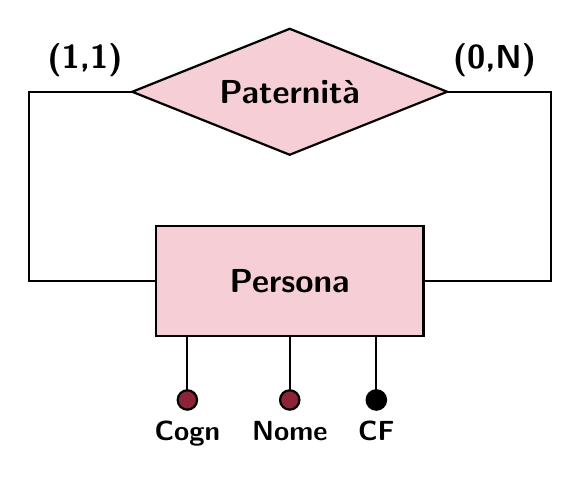
\begin{tikzpicture}[thick]
				\definecolor{softpink}{RGB}{245, 206, 214}
				\definecolor{darkred}{RGB}{140, 35, 55}
				
				\def\rx{2.0}
				\def\ry{0.8}
				
				% Entità: Persona
				\node[draw, fill=softpink, minimum width=3.4cm, minimum height=1.4cm, font=\sffamily\bfseries\large] (pers) at (0, 0) {Persona};
				
				% Relazione ricorsiva: Paternità
				\coordinate (cPat) at (0, 2.4);
				\draw[fill=softpink] (cPat) ++(0, \ry) -- ++(\rx, -\ry) -- ++(-\rx, -\ry) -- ++(-\rx, \ry) -- cycle;
				\node[font=\sffamily\bfseries\large] at (cPat) {Paternità};
				
				% Linee dell'anello ricorsivo modellate singolarmente
				\draw (pers.west) -- ++(-1.6, 0) -- ++(0, 2.4) -- ([xshift=-\rx cm]cPat);
				\draw (pers.east) -- ++(1.6, 0) -- ++(0, 2.4) -- ([xshift=\rx cm]cPat);
				
				% Cardinalità posizionate in modo indipendente
				\node[font=\sffamily\bfseries\large] at (-2.6, 2.8) {(1,1)};
				\node[font=\sffamily\bfseries\large] at (2.6, 2.8) {(0,N)};
				
				% Attributi dell'entità Persona
				\draw ([xshift=-1.3cm]pers.south) -- ++(0, -0.8) coordinate (aCogn);
				\filldraw[fill=darkred] (aCogn) circle (3.5pt) node[below=4pt, font=\sffamily\bfseries\normalsize] {Cogn};
				
				\draw (pers.south) -- ++(0, -0.8) coordinate (aNome);
				\filldraw[fill=darkred] (aNome) circle (3.5pt) node[below=4pt, font=\sffamily\bfseries\normalsize] {Nome};
				
				\draw ([xshift=1.1cm]pers.south) -- ++(0, -0.8) coordinate (aCF);
				\filldraw[fill=black] (aCF) circle (3.5pt) node[below=4pt, font=\sffamily\bfseries\normalsize] {CF};
			\end{tikzpicture}%
		}
		\caption{Associazione uno-a-molti ricorsiva.}
	\end{figure}
	Nel caso di questa associazione, si vogliono spendere due parole su entrambe le traduzioni in quanto potrebbero presentare delle criticità:
	\begin{enumerate}
		\item \textbf{Creazione di una tabella per la relazione}, e dunque si avrà lo schema
		\begin{center}
			Persona(\textbf{CF}, Nome, Cogn)\\
			Paternita(\textbf{Figlio}, \textit{Padre})
		\end{center}
		Si presti particolare attenzione alla scelta della chiave primaria nella tabella \texttt{Paternita}:
		\begin{itemize}
			\item Se avessimo scelto solo \textbf{Padre} ci saremmo trovati nella situazione in cui un padre può avere al più un figlio, chiaramente errata per lo schema rappresentato.
			
			\item Se avessimo scelto come chiave la coppia \textbf{Figlio, Padre} ci saremmo potuti trovare nella situazione in cui un figlio è associato a più di un padre (in quanto, fissando il figlio e modificando il padre si possono generare tuple differenti).
		\end{itemize}
		
		\item \textbf{Unificazione in una sola tabella}. In questo caso lo schema sarebbe stato semplicemente Persona(\textbf{CF}, Nome, Cogn, \textit{Padre}), dove \textit{Padre} rappresenta una chiave esterna.
		
		Si noti una criticità di questa implementazione: per come definito prima, il vincolo di integrità referenziale impone che i valori associati alla chiave esterna siano valori \textbf{esistenti} nella tabella di partenza. Siccome in questo caso l'associazione è ricorsiva, la tabella di partenza è la stessa di quella di arrivo. Dunque questo ci mette nella condizione in cui ci è sostanzialmente \textbf{impossibile} (almeno all'inizio) inserire delle persone all'interno della tabella, in quanto non potremmo associarle un padre.\\
		Ci sono due possibili soluzioni:
		\begin{enumerate}
			\item Disabilitare temporaneamente i controlli di integrità del DBMS, per permettere di inserire delle persone e successivamente riabilitarli per creare la corrispondenza effettiva.
			
			\item Impostare il valore della chiave esterna come non obbligatorio (\textbf{RISCHIOSO!!!}) e inserire il valore della chiave esterna solo \textit{dopo aver effettuato sufficienti inserimenti}.
		\end{enumerate}
	\end{enumerate}
	
	Vediamo di seguito un esempio anche con le associazioni n-arie molti-a-molti.
	\begin{figure}[H]
		\centering
		\resizebox{0.60\linewidth}{!}{%
			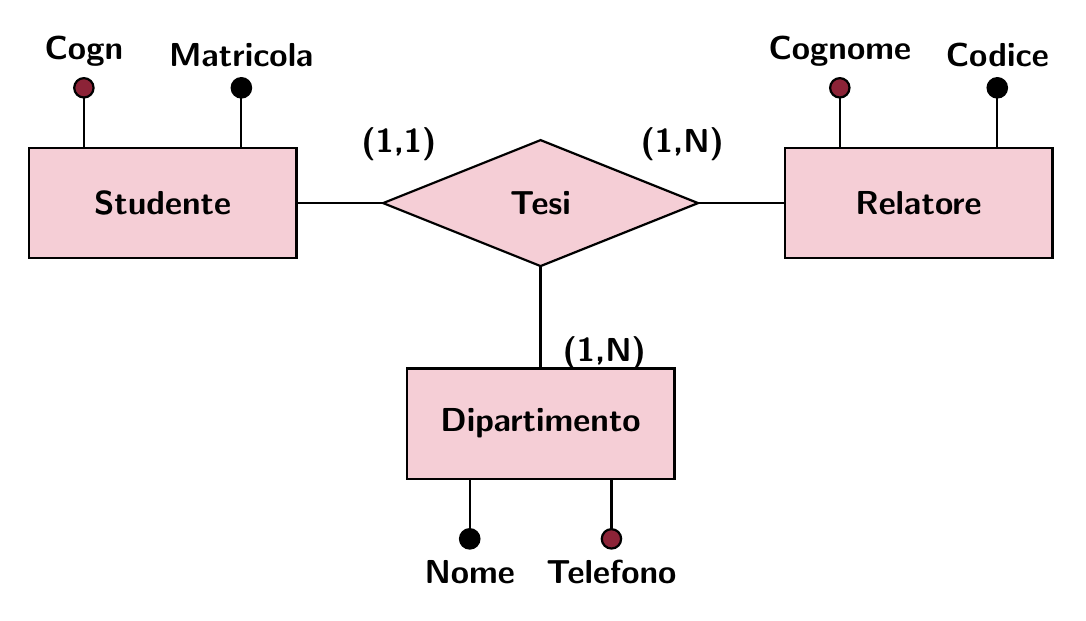
\begin{tikzpicture}[thick]
				\definecolor{softpink}{RGB}{245, 206, 214}
				\definecolor{darkred}{RGB}{140, 35, 55}
				
				\def\rx{2.0}
				\def\ry{0.8}
				
				% Coordinate centrali
				\coordinate (cTesi) at (4.8, 0);
				
				% Entità: Studente, Relatore, Dipartimento
				\node[draw, fill=softpink, minimum width=3.4cm, minimum height=1.4cm, font=\sffamily\bfseries\large] (stud) at (0, 0) {Studente};
				\node[draw, fill=softpink, minimum width=3.4cm, minimum height=1.4cm, font=\sffamily\bfseries\large] (rel)  at (9.6, 0) {Relatore};
				\node[draw, fill=softpink, minimum width=3.4cm, minimum height=1.4cm, font=\sffamily\bfseries\large] (dip)  at (4.8, -2.8) {Dipartimento};
				
				% Relazione ternaria: Tesi
				\draw[fill=softpink] (cTesi) ++(0, \ry) -- ++(\rx, -\ry) -- ++(-\rx, -\ry) -- ++(-\rx, \ry) -- cycle;
				\node[font=\sffamily\bfseries\large] at (cTesi) {Tesi};
				
				% Linee di collegamento tra entità e relazione
				\draw (stud.east) -- ([xshift=-\rx cm]cTesi);
				\draw ([xshift=\rx cm]cTesi) -- (rel.west);
				\draw ([yshift=-\ry cm]cTesi) -- (dip.north);
				
				% Cardinalità distanziate
				\node[font=\sffamily\bfseries\large] at (3.0, 0.75) {(1,1)};
				\node[font=\sffamily\bfseries\large] at (6.6, 0.75) {(1,N)};
				\node[font=\sffamily\bfseries\large, anchor=west] at (4.95, -1.9) {(1,N)};
				
				% Attributi dell'entità Studente
				\draw ([xshift=-1.0cm]stud.north) -- ++(0, 0.75) coordinate (aCognS);
				\filldraw[fill=darkred] (aCognS) circle (3.5pt) node[above=4pt, font=\sffamily\bfseries\large] {Cogn};
				
				\draw ([xshift=1.0cm]stud.north) -- ++(0, 0.75) coordinate (aMatr);
				\filldraw[fill=black] (aMatr) circle (3.5pt) node[above=4pt, font=\sffamily\bfseries\large] {Matricola};
				
				% Attributi dell'entità Relatore
				\draw ([xshift=-1.0cm]rel.north) -- ++(0, 0.75) coordinate (aCognR);
				\filldraw[fill=darkred] (aCognR) circle (3.5pt) node[above=4pt, font=\sffamily\bfseries\large] {Cognome};
				
				\draw ([xshift=1.0cm]rel.north) -- ++(0, 0.75) coordinate (aCodR);
				\filldraw[fill=black] (aCodR) circle (3.5pt) node[above=4pt, font=\sffamily\bfseries\large] {Codice};
				
				% Attributi dell'entità Dipartimento
				\draw ([xshift=-0.9cm]dip.south) -- ++(0, -0.75) coordinate (aNomeD);
				\filldraw[fill=black] (aNomeD) circle (3.5pt) node[below=4pt, font=\sffamily\bfseries\large] {Nome};
				
				\draw ([xshift=0.9cm]dip.south) -- ++(0, -0.75) coordinate (aTelD);
				\filldraw[fill=darkred] (aTelD) circle (3.5pt) node[below=4pt, font=\sffamily\bfseries\large] {Telefono};
			\end{tikzpicture}%
		}
		\caption{Associazione ternaria molti-a-molti.}
	\end{figure}
	
	Il trucco per le associazioni n-arie è \textit{leggerle a due a due}, dunque prendendo una coppia di entità e leggere l'associazione tra queste. Fare poi questo lavoro per tutte le entità coinvolte.
	Anche in questo caso la traduzione può avvenire in due modi:
	\begin{enumerate}
		\item \textbf{Creando la tabella per l'associazione}, ottenendo il seguente schema della base di dati:
		\begin{center}
			Studente(\textbf{Matricola}, Cogn)\\
			Relatore(\textbf{Codice}, Cogn)\\
			Dipartimento(\textbf{Nome}, Telefono)\\
			Tesi(\textbf{Studente}, \textit{Relatore}, \textit{Dipartimento})
		\end{center}
		Ci accorgiamo però che le tabelle \texttt{Studente} e \texttt{Tesi} hanno la stessa chiave primaria, e dunque conviene unificarle.
		
		\item \textbf{Unificare tutto in un'unica tabella}, ottenendo lo schema:
		\begin{center}
			Relatore(\textbf{Codice}, Cogn)\\
			Dipartimento(\textbf{Nome}, Telefono)\\
			Studente(\textbf{Matricola}, Cogn, \textit{Relatore}, \textit{Dipartimento})
		\end{center}
	\end{enumerate}
	
	\subsection{I valori NULL}
	I valori NULLI rappresentano mancanza di informazione oppure che un'informazione non è applicabile a quella n-upla. Vediamo un esempio con un'informazione che usiamo tutti i giorni: il numero di telefono.\\
	In una base di dati, il numero di telefono di una persona potrebbe assumere un valore nullo in diverse circostanze:
	\begin{itemize}
		\item La persona effettivamente non possiede un telefono cellulare e dunque neanche un numero.
		
		\item Non sappiamo se la persona abbia un numero di telefono.
		
		\item La persona ha un numero di telefono ma non lo conosciamo.
	\end{itemize}
	Nell'ottica della progettazione logica, dobbiamo stabilire questo vincolo (indicando che l'attributo può assumere valori NULL), ma in generale si tende a non utilizzare questa pratica, in quanto per la definizione di tupla questa deve possedere un valore per ogni attributo nello schema. Infatti, una possibile tecnica potrebbe essere quella di attribuire un valore di \textbf{default}.\\
	Ci rendiamo anche conto di come molti campi debbano categoricamente essere \textbf{obbligatori}. Si tratta solitamente dei campi che contengono informazioni fondamentali per l'identificazione della tupla (come ad esempio la matricola di uno studente, che ci permette di identificarlo univocamente) oppure il voto di uno studente ad un appello di esame (non usiamo questa informazione per identificare lo studente, ma si tratta di un'informazione fondamentale in una base di dati universitaria).
	\smallbreak
	
	Entrando più nello specifico del valore NULL, possiamo dire che:
	\begin{itemize}
		\item Si tratta di un valore \textbf{polimorfo}, cioè che non appartiene nello specifico a nessun dominio, ma può sostituire valori in qualsiasi dominio (ad esempio, se abbiamo degli attributi di tipo intero e stringhe, possiamo comunque inserire NULL come valore in quanto sarà compatibile con entrambi).
		
		\item Due valori NULL, anche se sullo stesso dominio, sono considerati \textbf{diversi}.
		
		\item \textbf{IMPORTANTE}! NULL $\neq$ 0.
	\end{itemize}
	
	\section{Vincoli di integrità}
	\begin{definizione}{Vincolo di integrità}{}
		Un \textbf{vincolo di integrità} è una proprietà che deve essere categoricamente rispettata da \textbf{ogni istanza} della base di dati, in quanto è strettamente legata allo schema di una relazione.
		\smallbreak
		
		Un'istanza della base di dati si dice \textbf{corretta} se soddisfa tutti i vincoli di integrità associati al suo schema.
	\end{definizione}
	
	I vincoli di integrità si possono suddividere in due tipologie:
	\begin{description}
		\item [Vincoli di integrità intra-relazionali:] sono \textbf{vincoli che si stabiliscono sugli attributi o sulle tuple di una singola relazione}. Alcuni esempi di questi sono:
		\begin{itemize}
			\item Vincolo di chiave primaria: attributo obbligatorio e mai nullo. Identifica univocamente una tupla all'interno della relazione.
			
			\item Vincolo di dominio: quando si restringe il dominio di un particolare attributo.
			
			\item Vincolo di unicità: stabilisce che il valore di un attributo in una tupla t deve essere univoco e non preso da nessun'altra tupla.
			
			\item Vincolo di obbligatorietà: stabilisce che un attributo deve necessariamente avere un valore.
		\end{itemize}
		
		\item[Vincoli di integrità inter-relazionali:] sono \textbf{vincoli che si stabiliscono tra relazioni diverse}, "collegando" ad esempio attributi con lo stesso dominio e creando un legame in base al valore assunto dai due attributi. Un esempio è il vincolo di chiave esterna che abbiamo citato qualche sezione fa.
	\end{description}
	
	Facciamo alcuni esempi concreti di violazione di vincoli, oppure di casi in cui si potrebbero imporre dei vincoli.
	\begin{tabella}{|c|c|c|c|c|}
		CodiceImp & Cognome & Ruolo & Assunzione & Dip\\\hline
		COD1 & Rossi & Analista & 1795 & 01\\\hline
		COD2 & Bianchi & Analista & 1990 & 05\\\hline
		COD2 & Neri & Amministratore & 1985 & 01\\
	\end{tabella}
	
	\begin{tabella}{|c|c|}
		CodiceDip & Nome\\\hline
		01 & Progettazione\\\hline
		02 & Amministrazione\\
	\end{tabella}
	
	Considerando quest'esempio di base di dati, ci sono molti problemi: vediamo dove risiedono.
	\begin{enumerate}
		\item L'impiegato \texttt{COD1} risulta avere anno di assunzione 1795. Ciò è chiaramente impossibile, e una possibile soluzione potrebbe essere stabilire un anno di assunzione minimo (\textit{vincolo di dominio}).
		
		\item L'impiegato "Bianchi" risulta appartenere al dipartimento di codice "05", che è tuttavia inesistente, in quanto non presente in alcuna tupla della tabella \texttt{Dipartimenti}. Questo si potrebbe risolvere stabilendo un \textit{vincolo di chiave esterna} tra l'attributo \texttt{Dip} di \texttt{Impiegato} e l'attributo \texttt{CodiceDip} di \texttt{Dipartimenti}.
		
		\item Vi è una duplicazione del codice identificativo per gli impiegati "Bianchi" e "Neri". Ciò si potrebbe risolvere imponendo un \textit{vincolo di unicità} sui valori della colonna \texttt{CodiceImp}.
	\end{enumerate}
	Ovviamente esistono tanti altri tipi di vincoli, e altrettanti modi per definirli nello schema della base di dati, ma li vedremo più nel dettaglio durante la creazione effettiva delle relazioni.
	
	\chapter{Algebra relazionale}
	L'algebra relazionale è un \textbf{linguaggio formale che si basa su modelli matematici utile per interrogare una base di dati relazionale}. Consiste in un insieme di operatori che agiscono su una singola relazione, detti appunto \textbf{unari}, e un insieme di attributi che agiscono su coppie di relazioni, per l'appunto \textbf{binari}. Il \textbf{risultato} di ognuna di queste operazioni è una \textbf{nuova relazione}.
	
	\begin{osservazione}{Algebra relazionale come linguaggio procedurale}{}
		L'algebra relazionale può essere anche vista come \textbf{linguaggio procedurale}, ovvero un linguaggio per cui si \textbf{esprimono in sequenza le operazioni da eseguire, come operare sulle relazioni e cosa estrarre da esse}.\\
		Questa è un'importante differenza con il linguaggio DQL con il quale effettueremo effettivamente le interrogazioni, che è invece un linguaggio \textbf{dichiarativo}, cioè dove noi non diciamo cosa fare al linguaggio ma solo cosa vogliamo ottenere (sarà poi il DBMS ad attuare le dovute operazioni per mostrarci il risultato richiesto).
	\end{osservazione}
	
	Di seguito elenchiamo i vari operatori dell'algebra relazionale, discutendoli poi più nel dettaglio in sezioni separate.
	
	\section{Proiezione}
	Si tratta di un \textbf{operatore unario} \textbf{che permette di selezionare da una relazione tutte le tuple limitando ciascuna ad un insieme di attributi specificato}.\\
	Formalmente parlando, data un'istanza di relazione $r$ con un insieme di attributi $X$, se effettuiamo una proiezione su $r$ sull'insieme $\{A_1, A_2, \dots, A_k\} \subseteq X$ otteniamo una nuova relazione che contiene tutte le tuple $t \in r$ ognuna ristretta agli attributi $\{A_1, A_2, \dots, A_k\}$.\\
	Corrisponde all'operatore \texttt{SELECT DISTINCT} del linguaggio DQL, che permette di specificare quali attributi della relazione vogliamo visionare come risultato della query.\\
	L'operazione di proiezione si indica con la notazione
	\[
		\pi_{A_1, A_2, \dots, A_k}(r)
	\]
	
	\begin{esempio}{Esempio di proiezione su una tabella "Clienti"}{}
		\begin{tabella}{|c|c|c|}
			Nome & C\# & Citta\\\hline
			Rossi & C1 & Roma\\\hline
			Rossi & C2 & Milano\\\hline
			Bianchi & C3 & Roma\\\hline
			Verdi & C4 & Roma\\
		\end{tabella}
		\vspace{1em}
		Supponiamo di voler sapere tutti i nomi dei clienti:
		\[
			\pi_{\text{Nome}}(\text{Clienti})
		\]
		La relazione risultante sarà
		\begin{tabellaSemplice}{|c|}
			Rossi\\\hline
			Bianchi\\\hline
			Verdi\\
		\end{tabellaSemplice}
		
		Ovviamente, dato che il risultato dell'operazione è a sua volta una relazione (di fatto un sottoinsieme), nella stessa colonna non potremo avere valori duplicati, ed ecco perché appare solo 1 volta "Rossi".
	\end{esempio}
	
	\begin{osservazione}{Come ottenere tutte le tuple}{}
		Come abbiamo visto, la proiezione è un'operazione insiemistica, e per tanto non mantiene duplicati. Se volessimo fare in modo che la relazione risultante dalla proiezione mostrasse tutte le tuple, anche quelle contenenti omonimi (ma questo discorso vale per qualsiasi istanza in cui si va ad usare un'operazione di proiezione) dovremmo includere anche la \textbf{chiave primaria} della relazione nell'insieme di attributi della proiezione.
		\smallbreak
		
		Questo avviene in quanto ricordiamo essere la chiave primaria di una tupla ad identificarla univocamente all'interno dell'istanza di relazione. Ed è proprio il motivo per cui quando inseriamo come unico attributo della selezione il campo "Nome", essendo quello l'unico diventerà lui la chiave primaria della nuova relazione, e dunque non saranno ammesse occorrenze duplicate.
	\end{osservazione}
	
	Possiamo dire che la proiezione compie un \textbf{taglio verticale} su una relazione, eliminando solo alcune colonne (e i relativi valori per ogni tupla) dalla relazione di partenza.
	
	\section{Selezione}
	Si tratta di un \textbf{operatore unario} che permette di \textbf{selezionare dalla relazione di partenza solo le tuple che rispettano una determinata condizione} $C$.\\
	Formalmente parlando, sia $r$ un istanza di relazione e $C$ una condizione proposizionale. L'operazione di selezione produce una nuova relazione in cui sono contenute tutte le tuple $t \in r$ per cui $C$ risulta vera.\\
	Quest'operazione è il corrispettivo della clausola \texttt{WHERE} nel linguaggio DQL.
	L'operazione di selezione si indica con la notazione
	\[
		\sigma_C(r)
	\]
	
	\begin{esempio}{Esempio di selezione su una tabella "Clienti"}{}
		\noindent
		\begin{minipage}[c]{0.44\textwidth}
			\centering
			\renewcommand{\arraystretch}{1.3}
			\begin{tabular}{|c|c|c|c|}
				\hline
				\rowcolor{BrickRed!60!white}
				Nome & C\# & Citt\`a & \dots\dots \\
				\hline
				Rossi   & C1 & Roma   & \dots\dots \\
				Rossi   & C2 & Milano & \dots\dots \\
				Rossi   & C3 & Roma   & \dots\dots \\
				Bianchi & C4 & Roma   & \dots\dots \\
				Verdi   & C5 & Roma   & \dots\dots \\
				\hline
			\end{tabular}
		\end{minipage}\hfill
		\begin{minipage}[c]{0.08\textwidth}
			\centering
			\begin{tikzpicture}
				\draw[->, >=stealth, very thick, rossoSapienza] (0,0) -- (0.8,0);
			\end{tikzpicture}
		\end{minipage}\hfill
		\begin{minipage}[c]{0.44\textwidth}
			\centering
			\renewcommand{\arraystretch}{1.3}
			\begin{tabular}{|c|c|c|c|}
				\hline
				\rowcolor{BrickRed!60!white}
				Nome & C\# & Citt\`a & \dots\dots \\
				\hline
				Rossi   & C1 & Roma & \dots\dots \\
				Rossi   & C3 & Roma & \dots\dots \\
				Bianchi & C4 & Roma & \dots\dots \\
				Verdi   & C5 & Roma & \dots\dots \\
				\hline
			\end{tabular}
		\end{minipage}
		
		\vspace{1em}
		La relazione di destra è la relazione risultante dall'operazione $\sigma_{\text{Citta = "Roma"}}(\text{Clienti})$.
	\end{esempio}
	
	\section{Unione}
	L'operatore di unione è un operatore binario che ci permette di costruire una nuova relazione che conterrà \textbf{tutte le tuple che appartengono ad entrambe le relazioni} (dunque tutte le tuple della prima e tutte le tuple della seconda).\\
	La definizione formale dell'operatore è proprio quella matematiche che ci aspetteremmo: date due istanze di relazione $r_1, r_2$, l'unione tra queste due relazioni è l'insieme $\{t \,|\, t \in r_1 \vee t \in r_2\}$.
	\smallbreak
	
	\begin{definizione}{Relazioni "union compatibili"}{}
		L'operazione di unione non è applicabile su qualsiasi coppia di relazioni. Due relazioni si dicono \textbf{union compatibili} se:
		\begin{itemize}
			\item \textbf{Hanno lo stesso numero di attributi}.
			
			\item \textbf{Hanno gli stessi domini} (in ordine).
		\end{itemize}
	\end{definizione}
	
	L'operazione è ugualmente chiamata \texttt{UNION} anche nel linguaggio DQL, e si indica con la seguente notazione:
	\[
		r_1 \cup r_2
	\]
	\begin{figure}[htbp]
		\centering
		\usetikzlibrary{patterns}
		\resizebox{0.40\linewidth}{!}{%
			\begin{tikzpicture}
				\fill[pattern=north east lines, pattern color=black] 
				(0,0) circle (1.2) 
				(1.4,0) circle (1.2);
				
				\draw[thick, rossoSapienza] (0,0) circle (1.2);
				\draw[thick, rossoSapienza] (1.4,0) circle (1.2);
				
				\node[font=\Large\itshape, rossoSapienza] at (-1.8, 0.4) {$r_1$};
				\node[font=\Large\itshape, rossoSapienza] at (3.2, 0.4) {$r_2$};
			\end{tikzpicture}%
		}
		\caption{Rappresentazione grafica dell'unione tra $r_1$ e $r_2$.}
		\label{fig:unione_relazioni}
	\end{figure}
	
	Di seguito un esempio di come risulta essere l'unione tra due relazioni, rispettivamente \texttt{Docenti} e \texttt{Amministrativi}.
	\begin{esempio}{Esempio di unione tra due relazioni}{}
		\noindent
		\begin{minipage}[t]{0.48\textwidth}
			\centering
			\renewcommand{\arraystretch}{1.3}
			\begin{tabular}{|c|c|c|}
				\hline
				\rowcolor{BrickRed!60!white}
				Nome & CodDoc & Dipartimento \\
				\hline
				Rossi   & D1 & Matematica \\
				Rossi   & D2 & Lettere    \\
				Bianchi & D3 & Matematica \\
				Verdi   & D4 & Lingue     \\
				\hline
			\end{tabular}
		\end{minipage}\hfill
		\begin{minipage}[t]{0.48\textwidth}
			\centering
			\renewcommand{\arraystretch}{1.3}
			\begin{tabular}{|c|c|c|}
				\hline
				\rowcolor{BrickRed!60!white}
				Nome & CodAmm & Dipartimento \\
				\hline
				Esposito & A1 & Lingue     \\
				Riccio   & A2 & Matematica \\
				Pierro   & A3 & Lettere    \\
				Verdi    & A4 & Lingue     \\
				Bianchi  & A5 & Lingue     \\
				\hline
			\end{tabular}
		\end{minipage}
		
		\vspace{1em}
		L'unione tra queste due relazioni risulta essere la seguente relazione:
		\begin{tabella}{|C|C|C|}
			Nome & Cod & Dipartimento \\
			\hline
			Rossi    & D1 & Matematica \\
			Rossi    & D2 & Lettere    \\
			Bianchi  & D3 & Matematica \\
			Verdi    & D4 & Lingue     \\
			Esposito & A1 & Lingue     \\
			Riccio   & A2 & Matematica \\
			Pierro   & A3 & Lettere    \\
			Verdi    & A4 & Lingue     \\
			Bianchi  & A5 & Lingue     \\
		\end{tabella}
		
	\end{esempio}
	
	\begin{osservazione}{Coerenza degli attributi nell'unione}{}
		E' doveroso fare un'osservazione. Due relazioni definite rispettivamente come \texttt{Studenti(Nome, Eta)} e \texttt{Professore(Nome, NumeroTelefono)} sono di fatto union compatibili: il campo \texttt{Nome} è in entrambi i casi un attributo di dominio \texttt{String}, e gli attributi \texttt{Eta} e \texttt{NumeroTelefono} sono entrambi numeri interi. Ci rendiamo conto che però il significato dei due attributi sia diverso, nonostante condividano lo stesso dominio. Dunque la relazione risultante sarà ambigua o incoerente nel campo di dominio \texttt{Intero}.
	\end{osservazione}
	
	\begin{osservazione}{Come rendere due relazioni Union compatibili}{}
		
		\begin{minipage}[t]{0.45\textwidth}
			\centering
			\renewcommand{\arraystretch}{1.3}
			\begin{tabular}{|c|c|c|}
				\hline
				\rowcolor{BrickRed!60!white}
				Nome & CodDoc & Dipartimento \\
				\hline
				Rossi   & D1 & Matematica \\
				Rossi   & D2 & Lettere    \\
				Bianchi & D3 & Matematica \\
				Verdi   & D4 & Lingue     \\
				\hline
			\end{tabular}
		\end{minipage}\hfill
		\begin{minipage}[t]{0.53\textwidth}
			\centering
			\renewcommand{\arraystretch}{1.3}
			\begin{tabular}{|c|c|c|c|}
				\hline
				\rowcolor{BrickRed!60!white}
				Nome & CodAmm & Dipartimento & Stip \\
				\hline
				Esposito & A1 & Lingue     & 1250 \\
				Riccio   & A2 & Matematica & 2000 \\
				Pierro   & A3 & Lettere    & 1000 \\
				\hline
			\end{tabular}
		\end{minipage}
		
		\vspace{1em}
		Ora come ora, queste relazioni non risultano essere Union compatibili, in quanto la relazione di destra presenta un attributo in più. Se però prendessimo come relazione quella risultante da $\pi_{\text{Nome, CodAmm, Dipartimento}}(\text{Amministrativi})$ otterremmo una nuova relazione che sarà adesso Union compatibile con quella di sinistra.
		\smallbreak
		
		Il succo della questione è: \textbf{possiamo rendere due relazioni Union compatibili considerando la relazione risultante dalla proiezione di una di queste}. Ovviamente supponendo che abbiano almeno un dominio comune, altrimenti ciò rimarrebbe impossibile.
	\end{osservazione}
	
	\section{Differenza}
	Si tratta di un operatore \textbf{binario} che si può applicare tra due relazioni che sono già "Union compatibili". Il risultato dell'operazione è una \textbf{relazione che contiene tutti gli elementi della prima relazione che non sono anche nella seconda}.\\
	Definendo quest'operazione matematicamente, abbiamo che la differenza tra una relazione $r_1, r_2$ è l'insieme $\{t \, |\, t \in r_1 wedge t \notin r_2\}$.\\
	Tale operazione si indica nel seguente modo
	\[
		r_1 - r_2
	\]
	\begin{figure}[htbp]
		\centering
		\resizebox{0.40\linewidth}{!}{%
			\begin{tikzpicture}
				\begin{scope}
					% Ritaglia solo l'area appartenente al cerchio r1
					\clip (0,0) circle (1.2);
					% Riempie con il tratteggio
					\fill[pattern=north east lines, pattern color=black] (0,0) circle (1.2);
					% Cancella la porzione che si sovrappone a r2 per ottenere la differenza (r1 - r2)
					\fill[white] (1.4,0) circle (1.2);
				\end{scope}
				
				% Bordi dei due insiemi
				\draw[thick, rossoSapienza] (0,0) circle (1.2);
				\draw[thick, rossoSapienza] (1.4,0) circle (1.2);
				
				% Etichette degli insiemi
				\node[font=\Large\itshape, rossoSapienza] at (-1.8, 0.4) {$r_1$};
				\node[font=\Large\itshape, rossoSapienza] at (3.2, 0.4) {$r_2$};
			\end{tikzpicture}%
		}
		\caption{Differenza insiemistica tra le relazioni $r_1$ e $r_2$ ($r_1 - r_2$).}
		\label{fig:differenza_relazioni}
	\end{figure}
	
	\begin{esempio}{Esempio di differenza tra due relazioni}{}
		Consideriamo le seguenti relazioni, \texttt{Studenti} e \texttt{Amministrativi}:\\
		\begin{minipage}[t]{0.48\textwidth}
			\vspace{0.1em}
			\centering
			\renewcommand{\arraystretch}{1.3}
			\begin{tabular}{|c|c|c|}
				\hline
				\rowcolor{BrickRed!60!white}
				Nome & CodFiscale & Dipartimento \\
				\hline
				Rossi   & C1 & Matematica \\
				Rossi   & C2 & Lettere    \\
				Bianchi & C3 & Matematica \\
				Verdi   & C4 & Lingue     \\
				\hline
			\end{tabular}
		\end{minipage}\hfill
		\begin{minipage}[t]{0.48\textwidth}
			\vspace{0.1em}
			\centering
			\renewcommand{\arraystretch}{1.3}
			\begin{tabular}{|c|c|c|}
				\hline
				\rowcolor{BrickRed!60!white}
				Nome & CodFiscale & Dipartimento \\
				\hline
				Esposito & C5 & Lettere    \\
				Riccio   & C6 & Matematica \\
				Pierro   & C7 & Lingue     \\
				Bianchi  & C3 & Matematica \\
				\hline
			\end{tabular}
		\end{minipage}
		
		\vspace{1em}
		La differenza tra relazioni \textbf{non è un'operazione commutativa}. Dunque fare \texttt{Studenti - Amministrativi} è diverso dal fare \texttt{Amministrativi - Studenti}.\\
		Di seguito vediamo entrambi i risultati:\\
		\begin{minipage}[t]{0.48\textwidth}
			\vspace{0.1em}
			\centering
			\renewcommand{\arraystretch}{1.3}
			\begin{tabular}{|c|c|c|}
				\hline
				\rowcolor{BrickRed!60!white}
				Nome & CodFiscale & Dipartimento \\
				\hline
				Rossi & C1 & Matematica \\
				Rossi & C2 & Lettere    \\
				Verdi & C4 & Lingue     \\
				\hline
			\end{tabular}
		\end{minipage}\hfill
		\begin{minipage}[t]{0.48\textwidth}
			\vspace{0.1em}
			\centering
			\renewcommand{\arraystretch}{1.3}
			\begin{tabular}{|c|c|c|}
				\hline
				\rowcolor{BrickRed!60!white}
				Nome & CodFiscale & Dipartimento \\
				\hline
				Esposito & C5 & Lettere    \\
				Riccio   & C6 & Matematica \\
				Pierro   & C7 & Lingue     \\
				\hline
			\end{tabular}
		\end{minipage}
		
		\vspace{1em}
		A sinistra abbiamo la relazione \texttt{Studenti - Amministrativi}, che contiene al suo interno \textit{tutti gli studenti tranne quelli che sono anche amministrativi}.\\
		A destra abbiamo la relazione \texttt{Amministrativi - Studenti} che contiene \textit{tutti gli amministrativi tranne quelli che sono anche studenti}.
	\end{esempio}
	
	\section{Intersezione}
	Per quanto si potrebbe pensare all'intersezione come un operatore primitivo, esso è in realtà un operatore derivato dalla seguente operazione insiemistica: $r_1 - (r_1 - r_2)$.\\
	Il risultato dell'intersezione tra due relazioni è una nuova relazione che contiene \textbf{solo le tuple comuni ad entrambe le relazioni}. Formalmente la definiremmo come $\{t \, |\, t \in r_1 \wedge t \in r_2\}$.
	L'operazione di intersezione tra due relazioni si denota nel seguente modo:
	\[
		r_1 \cap r_2
	\]
	\begin{figure}[htbp]
		\centering
		\resizebox{0.40\linewidth}{!}{%
			\begin{tikzpicture}
				\begin{scope}
					% Ritaglia l'area di intersezione tra i due cerchi
					\clip (0,0) circle (1.2);
					\fill[pattern=north east lines, pattern color=black] (1.4,0) circle (1.2);
				\end{scope}
				
				% Bordi dei due insiemi
				\draw[thick, rossoSapienza] (0,0) circle (1.2);
				\draw[thick, rossoSapienza] (1.4,0) circle (1.2);
				
				% Etichette degli insiemi
				\node[font=\Large\itshape, rossoSapienza] at (-1.8, 0.4) {$r_1$};
				\node[font=\Large\itshape, rossoSapienza] at (3.2, 0.4) {$r_2$};
			\end{tikzpicture}%
		}
		\caption{Intersezione tra le relazioni $r_1$ e $r_2$ ($r_1 \cap r_2$).}
		\label{fig:intersezione_relazioni}
	\end{figure}
	
	\begin{esempio}{Esempio di intersezione tra due relazioni}{}
		Consideriamo le precedenti relazioni \texttt{Studenti} e \texttt{Amministrativi}:\\
		\begin{minipage}[t]{0.48\textwidth}
			\vspace{0.1em}
			\centering
			\renewcommand{\arraystretch}{1.3}
			\begin{tabular}{|c|c|c|}
				\hline
				\rowcolor{BrickRed!60!white}
				Nome & CodFiscale & Dipartimento \\
				\hline
				Rossi   & C1 & Matematica \\
				Rossi   & C2 & Lettere    \\
				Bianchi & C3 & Matematica \\
				Verdi   & C4 & Lingue     \\
				\hline
			\end{tabular}
		\end{minipage}\hfill
		\begin{minipage}[t]{0.48\textwidth}
			\vspace{0.1em}
			\centering
			\renewcommand{\arraystretch}{1.3}
			\begin{tabular}{|c|c|c|}
				\hline
				\rowcolor{BrickRed!60!white}
				Nome & CodFiscale & Dipartimento \\
				\hline
				Esposito & C5 & Lettere    \\
				Riccio   & C6 & Matematica \\
				Pierro   & C7 & Lingue     \\
				Bianchi  & C3 & Matematica \\
				\hline
			\end{tabular}
		\end{minipage}
		
		\vspace{1em}
		L'intersezione tra relazioni è ovviamente un'operazione commutativa, in quanto prende i record che si trovano in entrambe le relazioni. Il risultato dunque dell'intersezione delle precedenti relazioni sarà dunque l'unico studente che è sia \texttt{Studente} che \texttt{Amministrativo}.
		
		\begin{center}
			\renewcommand{\arraystretch}{1.3}
			\begin{tabular}{|c|c|c|}
				\hline
				\rowcolor{BrickRed!60!white}
				Nome & CodFiscale & Dipartimento \\
				\hline
				Bianchi & C3 & Matematica \\
				\hline
			\end{tabular}
		\end{center}
	\end{esempio}
	
	\section{Prodotto cartesiano}
	L'operazione di prodotto cartesiano tra due istanze di relazione funziona esattamente come il prodotto cartesiano tra due insiemi: si ottengono tutte le n-uple della prima relazione concatenate a quelle della seconda relazione. Abbiamo già parlato di prodotto cartesiano quando definivamo il concetto stesso di \textit{relazione}, dunque ci limiteremo solo a dire che il prodotto cartesiano tra una relazione $r_1$ e una relazione $r_2$ si indica nel seguente modo:
	\[
		r_1 \times r_2
	\]
	Vedendo un esempio più concreto, supponiamo di avere una tabella \texttt{Docenti} e una tabella \texttt{Corsi}.\\
	\begin{minipage}[t]{0.48\textwidth}
		\vspace{0.5em}
		\centering
		\renewcommand{\arraystretch}{1.3}
		\begin{tabular}{|c|c|c|}
			\hline
			\rowcolor{BrickRed!60!white}
			ID\_Docente & Cognome & CodCorso \\
			\hline
			D1 & De Marsico & C01\\\hline
			D2 & Pirri & C03\\\hline
		\end{tabular}
	\end{minipage}\hfill
	\begin{minipage}[t]{0.48\textwidth}
		\vspace{0.5em}
		\centering
		\renewcommand{\arraystretch}{1.3}
		\begin{tabular}{|c|c|c|}
			\hline
			\rowcolor{BrickRed!60!white}
			CodCorso & NomeCorso\\
			\hline
			C01 & Basi di dati\\\hline
			C02 & Algoritmi \\\hline
			C03 & Reti\\\hline
		\end{tabular}
	\end{minipage}
	
	\vspace{1em}
	Il prodotto cartesiano tra queste due tabelle risulta essere il seguente:\\
	\begin{tabella}{|c|c|c|c|c|}
		ID\_Docente & Cognome & CodCorso & NomeCorso \\\hline
		D1 & De Marsico & C01 & Basi di Dati \\\hline
		D1 & De Marsico & C02 & Algoritmi \\\hline
		D1 & De Marsico & C03 & Reti \\\hline
		D2 & Pirri & C01 & Basi di Dati \\\hline
		D2 & Pirri & C02 & Algoritmi \\\hline
		D2 & Pirri & C03 & Reti \\\hline
	\end{tabella}
	Come vediamo, dal prodotto cartesiano di queste due tabella abbiamo ottenuto una combinazione di tutte le istanze di docente con tutte le possibili istanze di corso. Tuttavia, come vediamo, avendo attributi con lo stesso nome, come riusciamo a determinare quale attributo è associato a quale relazione? E come facciamo a capire quale corrispondenza risulta veritiera?
	
	\section{Ridenominazione}
	A tal proposito, introduciamo l'operatore di \textbf{ridenominazione}, che è l'unico che agisce sullo schema della relazione. Il punto di questo operatore è proprio modificare il nome della relazione e degli attributi al suo interno, proprio per evitare casi del genere in cui vi è presente un attributo che nelle relazioni di partenza ha lo stesso nome.\\
	L'operazione di ridenominazione ha la seguente sintassi:
	\[
		\text{NuovoNomeRelazione} = \rho_{\text{NuovoNome1, NuovoNome2, \dots $\leftarrow$ Nome1, Nome2, \dots (R)}}
	\]
	dove "NuovoNome$(i)$" indica il nuovo nome che si vuole dare agli attributi nella nuova relazione.
	\smallbreak
	
	Dunque per porre un rimedio alla situazione precedente, si potrebbe ad esempio cambiare il nome dell'attributo che si riferisce al corso nella tabella \texttt{Docenti}, ad esempio nel seguente modo: $\text{DocentiNuovo} = \rho_{\text{CodCorsoInsegnato <- CodCorso(R)}}$. Avendo ridenominato l'attributo \texttt{CodCorso} della tabella \texttt{Docenti} possiamo effettuare il prodotto cartesiano senza il rischio di perdita di informazioni.\\
	Effettuando il prodotto cartesiano, il risultato sarà adesso:
	\begin{tabella}{|c|c|c|c|c|}
		ID\_Docente & Cognome & CodCorsoInsegnato & CodCorso & NomeCorso \\\hline
		D1 & De Marsico & C01 & C01 & Basi di Dati \\\hline
		D1 & De Marsico & C01 & C02 & Algoritmi \\\hline
		D1 & De Marsico & C01 & C03 & Reti \\\hline
		D2 & Pirri & C03 & C01 & Basi di Dati \\\hline
		D2 & Pirri & C03 & C02 & Algoritmi \\\hline
		D2 & Pirri & C03 & C03 & Reti \\\hline
	\end{tabella}
	Notiamo però adesso che c'è una discrepanza di valori: in alcune righe, il codice del corso insegnato dal docente non risulta essere lo stesso di quello corrispondente nella tupla. Basta ad esempio vedere la seconda e la terza tupla: per la tabella docenti, noi sappiamo che il docente di codice \texttt{D1} insegna il corso di codice \texttt{C01}; tuttavia nelle righe 2 e 3 il docente \texttt{D1} risulta avere una corrispondenza con i corsi di codice \texttt{C02} e \texttt{C03}.
	\begin{corollario}{Correttezza di una query che coinvolge più tabelle}{}
		Quando enunciato di seguito deve diventare un mantra per tutte le volte che si dovrà scrivere una query in cui vengono coinvolte più tabelle: se queste hanno un dominio comune che rappresenta la stessa informazione (come \texttt{CodCorso} nell'esempio antecedente) è \textit{strettamente necessario} \textbf{eguagliare quei due valori in modo da mantenere all'interno della tabella risultante solo i record che contengono la corrispondenza corretta}.
	\end{corollario}
	Dunque, nell'esempio precedente, se volessimo ottenere la tabella contenente solo le informazioni coerenti, l'operazione da fare dovrà essere una selezione delle righe in cui \texttt{CodCorsoInsegnato = CodCorso}.
	\[
		\sigma_{\text{CodCorsoInsegnato = CodCorso}}(\text{Docenti} \times \text{Corsi})
	\]
	Ottenendo dunque la seguente relazione:
	\begin{tabella}{|c|c|c|c|c|}
		ID\_Docente & Cognome & CodCorsoInsegnato & CodCorso & NomeCorso \\\hline
		D1 & De Marsico & C01 & C01 & Basi di Dati \\\hline
		D2 & Pirri & C03 & C03 & Reti \\\hline
	\end{tabella}
	Dove, come vediamo, abbiamo la duplicazione dell'attributo codice corso (seppur con nome diverso, il valore di quel campo è sostanzialmente duplicato). Seppur questo non sia un errore, potremmo decidere di omettere uno dei due attributi per garantire un risultato più carino. Si può ottenere con una semplice proiezione:
	\[
		\pi_{\text{ID\_Docente, Cognome, CodCorsoInsegnato, NomeCorso}}(\sigma_{\text{CodCorsoInsegnato = CodCorso}}(\text{Docenti} \times \text{Corsi}))
	\]
	Ottenendo così infine la tabella
	\begin{tabella}{|c|c|c|c|}
		ID\_Docente & Cognome & CodCorsoInsegnato & NomeCorso \\\hline
		D1 & De Marsico & C01 & Basi di Dati \\\hline
		D2 & Pirri & C03 & Reti \\\hline
	\end{tabella}
	
	\section{Join naturale}
	Fatte tutte queste considerazioni sul prodotto cartesiano, sulla necessità di ridenominare gli attributi e sulla stretta necessità di eguagliare due domini che rappresentano la stessa informazione per garantire la coerenza dei dati, introduciamo l'operatore dell'algebra relazionale che accorpa tutte queste operazioni: il \textbf{join naturale}.\\
	L'operazione di join naturale funziona esattamente come tutto il processo visto precedentemente:
	\begin{enumerate}
		\item Fa il prodotto cartesiano tra due relazioni.
		\item Di questo prodotto cartesiano, se specifichiamo due domini comuni che condividono la stessa informazione, verranno selezionate solo le tuple che hanno valore uguale in quei due attributi.
	\end{enumerate}
	Tale operazione è infatti definita come segue:
	\[
		r_1 \bowtie r_2 := \pi_{XY}(\sigma_C(r_1 \times r_2))
	\]
	\begin{osservazione}{Funzionamento del Join naturale}{}
		L'operazione di join naturale funziona ad una sola condizione: che i \textbf{due attributi condividenti dominio e "scope" informativo abbiano lo stesso nome in entrambe le due relazioni}. Dunque nell'esempio precedente non sarebbe servito a nulla usare il join naturale, a meno che noi non avessimo usato la ridenominazione per rendere i nomi degli attributi uguali.
		\smallbreak
		
		Nota che il risultato di un'operazione di Join naturale potrebbe tranquillamente essere una \textbf{relazione vuota}, in caso di \textbf{mancate corrispondenze tra i valori delle tuple}.
	\end{osservazione}
	
	\begin{osservazione}{Importanza dell'ordine delle operazioni}{}
		Si nota come l'ordine in cui vengono eseguite i vari operatori in un'interrogazione complessa è fondamentale, in quanto da ciò potrebbe cambiare l'efficienza dell'interrogazione. Ovviamente tutti i DBMS relazionali moderni implementano già le interrogazioni eseguendo le operazioni nell'ordine più efficiente. Tuttavia è importante notare come, ad esempio, effettuare una selezione delle tuple compatibili \textbf{prima} di fare il prodotto cartesiano sia un risparmio particolarmente sostanzioso, in quanto si riduce il numero di tuple che vanno combinate l'un l'altra.
	\end{osservazione}
	
	\section{Theta Join}
	L'operazione di Join naturale è un'operazione potentissima, che ci permette finalmente di costruire gli effettivi collegamenti mediante valori tra le relazioni. Tuttavia presenta alcune limitazioni:
	\begin{itemize}
		\item I due attributi che condividono il dominio devono avere lo stesso nome (risolvibile con la ridenominazione ma è un'operazione costosa).
		
		\item Gli attributi omonimi possono esclusivamente essere uguagliati e non confrontati in alcun altro modo.
		
		\item Elimina le colonne duplicate, dunque di quelle che consentono di creare la corrispondenza ne mantiene una sola.
	\end{itemize}
	A tal proposito, si è deciso di definire un operatore chiamato $\theta$-Join (Theta Join) che rifinisce tali aspetti:
	\begin{itemize}
		\item Non è necessario che gli attributi colleganti abbiano lo stesso nome.
		
		\item Il confronto tra questi attributi è definibile sotto qualsiasi operatore matematico di confronto.
		
		\item Mantiene tutte le colonne delle relazioni di partenza, dunque non applica alcuna proiezione sul risultato finale.
	\end{itemize}
	La definizione formale di tale operazione è la seguente:
	\[
		r_1 \bowtie_{A\theta B} r_2 := \sigma_{A \theta B}(r_1 \times r_2)
	\]
	
	\section{Quantificatori unari e globali}
	Finora tutte le operazioni di interrogazione che abbiamo definito e svolto sulle nostre relazioni si sono basate su delle richieste molto simili: \textit{trovare tutte le istanze di ... tali che esiste almeno un ...}\\
	Detto così è un po' astratto, però con un esempio forse si chiarirà il concetto: \textit{trovare tutti gli studenti che hanno superato almeno un esame}. Come vediamo, ci viene chiesto SE ESISTONO gli studenti con almeno un esame, e memorizzarli in una relazione. Dunque sappiamo come operare: scorriamo tutte le tuple di una relazione e appena troviamo una tupla con \texttt{Superato = True}, allora prendiamo codice e nome di quello studente e li inseriamo come tupla nella nuova relazione.
	
	Insomma, finora tutte le nostre interrogazioni si sono basate sulla costante logica di \textbf{scansionare una per una le tuple e decidere lì sul momento se quella tupla fosse compatibile o meno}. Matematicamente, questo equivale al quantificatore essenziale $\exists$.
	\smallbreak
	
	Vogliamo ora spostare il nostro ragionamento: e se ci fosse stato chiesto \textit{tutti gli studenti che non hanno partecipato all'esame}? Oppure gli studenti \textit{che non l'hanno mai superato?} Come vediamo, la situazione diventa diversa:
	\begin{itemize}
		\item Nel primo esempio, se non vedo uno studente fino alla penultima riga non posso dare per scontato che non si sia presentato a quell'esame, dato che potrebbe essere presente come ultima tupla della relazione.
		
		\item Nel secondo esempio, invece, se leggo che lo studente con codice 003 non ha superato l'esame in una tupla, non posso decretare direttamente che non lo abbia mai superato e dunque inserirlo nella relazione di destinazione, in quanto potrebbe esserci una tupla successiva in cui viene invece detto che lo studente ha superato tale esame.
	\end{itemize}
	Per questo tipo di interrogazioni, dobbiamo cambiare il modo di ragionare: non più con il quantificatore $\exists$, bensì con il quantificatore $\forall$ oppure $\nexists$.\\
	
	Ragionare secondo quantificatori globali, che dunque prendono in esempio tanti elementi insieme, è sempre più difficile. Potremmo dunque ragionare al contrario, \textbf{negando} il quantificatore globale per ottenerne uno unario.
	\begin{definizione}{Negazione di $\forall$}{}
		Data una proposizione del tipo "$\forall$ oggetti VALE condizione", la sua \textbf{negazione} sarà la proposizione "$\mathbf{\exists}$ \textbf{oggetto per cui NON VALE CONDIZIONE}".
		\smallbreak
		
		Facciamo un esempio pratico: la negazione della frase "Tutti i miei amici si chiamano Francesco" è "Ho ALMENO UN amico che non si chiama Francesco". Come vediamo, siamo riusciti a trasformare un quantificatore globale in uno unario semplicemente negando la proposizione.
	\end{definizione}
	
	Per testarne il funzionamento, proviamolo su una richiesta vera.
	\begin{esempio}{Interrogaione con negazione di quantificatori globali}{}
		Supponiamo la richiesta sia "\textit{Trovare tutti gli studenti che hanno superato tutti gli esami a cui hanno partecipato}".\\
		Se fossimo rimasti con la mentalità precedente, sarebbe stato un disastro: per ogni studente avremmo dovuto memorizzare se ha passato un esame e solo se tutti fossero stati veri avremmo potuto metterlo nella nuova relazione.
		\smallbreak
		
		Adesso sappiamo però che la negazione ci è amica, e dunque la richiesta risulta esser equivalente a "\textit{Studenti che NON SONO MAI STATI BOCCIATI}". E qui la soluzione diventa banale: prendiamo la relazione ottenuta dalla Theta Join tra \texttt{Studenti} ed \texttt{Esami} e verifichiamo l'esito dell'esame per ogni tupla: se leggiamo \texttt{Esito = "Bocciato"}, allora questa tupla \textbf{non deve stare nella relazione richiesta}. Tuttavia, dato che stiamo ragionando al \textbf{complemento}, dovremo memorizzare questa tupla in una \textbf{relazione contenente solo gli studenti che non rispettano la condizione di partenza}.\\
		A quel punto, scansionate tutte le tuple, prendiamo la \textbf{relazione studenti di partenza e applichiamo la differenza con la relazione degli studenti bocciati almeno una volta}: il risultato di tale operazione insiemistica sarà anche la risposta alla nostra query.
	\end{esempio}
	
	In altri casi, a seconda di come è stata costruita la base di dati, potremmo ritrovarci che le informazioni per una query siano tutte nella stessa tabella, però appartenenti a tuple diverse che devono essere collegate l'un l'altra. Di seguito si presenta un esempio.
	\begin{esempio}{Interrogazione con Auto-Join}{}
		Supponiamo di avere una relazione \texttt{Impiegato} con il seguente schema \texttt{(Codice (PK), Cognome, Stipendio, CodCapo (FK))} e di voler ottenere \textit{tutti gli impiegati che hanno uno stipendio maggiore di quello del loro capo}. All'interno della relazione \texttt{Impiegato} sono infatti memorizzati anche i capi.
		\smallbreak
		
		Il fatto che le informazioni siano tutte nella stessa relazione non deve spaventarci, in quanto possiamo ragionare in maniera quasi completamente uguale a quando usavamo due relazioni: facciamo la Join tra le due relazioni ed estraiamo le informazioni.\\
		L'unico cambiamento nei casi delle Auto-Join risiede nel fatto che, essendo la stessa tabella, avremo i campi \textit{tutti con lo stesso nome}, e dunque molto probabilmente si verificheranno problemi di correttezza dei dati. La soluzione è quindi rinominare una delle due tabelle e i suoi campi.
		\begin{enumerate}
			\item Creiamo una copia ridenominata per la tabella contenente tutti i capi.
			\[
				\text{Capi} = \rho_{\text{CodC, CognC, StipC, CC} \leftarrow \text{Codice, Cognome, Stipendio, CodCapo}}(\text{Impiegato})
			\]
			
			\item Eseguiamo il Theta-Join tra la relazione \texttt{Impiegati} e la nuova relazione \texttt{Capi}.
			\[
				R_1 = \text{Impiegati} \bowtie_{\text{CodCapo} = \text{CodC} \land \text{Stipendio} > \text{StipC}} \text{Capi}
			\]
			
			\item Solo per un output più carino, eseguiamo una proiezione per estrarre solo codice e cognome di tale impiegato
			\[
				R_{\text{finale}} = \pi_{\text{Codice, Cognome}}(\text{R}_1)
			\]
		\end{enumerate}
	\end{esempio}
	
	\begin{esempio}{Query complessa con Auto-Join}{}
		Se invece, sempre in riferimento allo schema di relazione precedente, volessimo ottenere \textit{codice e cognome dei capi che guadagnano più di tutti i loro dipendenti}, dovremmo usare la struttura a doppia negazione.
		
		\begin{enumerate}
			\item Otteniamo la tabella di tutti i capi. Supponiamo di avere la relazione \texttt{Capi} definita come prima, e anche la relazione $R_1$ definita come Theta-Join tra impiegati e i loro capi. Per estrarre adesso solo i capi, cioè nome e cognome di ogni capo, ci basta fare una proiezione su questa relazione:
			\[
				\text{TuttiCapi} = \pi_{\text{CodC, CognC}}(\text{R}_1)
			\]
			Ci servirà per l'ultimo passaggio.
			
			\item Adesso dobbiamo ottenere tutti i capi che guadagnano più di \textit{tutti} i propri dipendenti. Questo si ottiene negando la proposizione, e dunque equivale a trovare \textbf{almeno un capo che guadagna meno di un suo dipendente}.
			\[
				\text{CapiScartati} = \text{Impiegato} \bowtie_{\text{CodCapo} = \text{CodC} \land \text{Stipendio} >= \text{StipC}}(\text{Capo})
			\]
			
			\item Adesso, dall'insieme di tutti i capi che abbiamo trovato nel primo passaggio, possiamo rimuovere quelli che non rispettano la richiesta iniziale, semplicemente con l'operatore di differenza.
			\[
				R_{\text{finale}} = \text{Capi} - \text{CapiScartati}
			\]
		\end{enumerate}
	\end{esempio}
	
	\chapter{Il linguaggio SQL}
	Al fine di creare i database, le tabelle, stabilire i vincoli tra queste ed effettuare operazioni di interrogazione sui dati era necessario un apposito linguaggio con cui fare tutto questo.\\
	Nasce così \textbf{SQL (Structured Query Language)}, il linguaggio diventato ormai di riferimento per tutti i DBMS moderni.
	\begin{definizione}{Sottolinguaggi di SQL}{}
		Il linguaggio SQL è un grande contenitore di moltissime istruzioni di vario genere. Nonostante la suddivisione logica di queste istruzioni non sia importante ai fini del calcolo, si tratta comunque di una nozione utile ai fini della progettazione o dell'uso di un DBMS.\\
		Le varie istruzioni del linguaggio SQL si suddividono in 4 sottolinguaggi:
		\begin{itemize}
			\item \textbf{DDL (Data Definition Language)}: contiene tutte le istruzioni che permettono la creazione/modifica/eliminazione di database e tabelle (es: \texttt{CREATE TABLE (...), CREATE DATABASE ..., ...}).
			
			\item \textbf{DML (Data Manipulation Language)}: comprende le istruzioni utili alla manipolazione dei dati all'interno delle tabelle, permettendo ad esempio istruzioni di inserimento, modifica o cancellazione di un dato (es: \texttt{INSERT INTO ... VALUES (...)}).
			
			\item \textbf{DQL (Data Query Language)}: si tratta del linguaggio che comprende tutte le istruzioni utili all'interrogazione dei dati (es: \texttt{SELECT ... FROM ... WHERE ...}).
			
			\item \textbf{DCL (Data Control Language)}: gestisce i permessi utente e limita l'accesso ai dati (\texttt{GRANT, REVOKE, ...}).
		\end{itemize}
	\end{definizione}
	
	\section{Il linguaggio di definizione dati: DDL}
	Nella seguente sezione andremo ad analizzare tutte le operazioni fondamentali che riguardano il linguaggio DDL per la creazione, modifica, cancellazione di tabelle, definizioni di dati e domini, creazione di vincoli intra e inter-relazionali.
	
	\subsection{Domini di dati}
	Come abbiamo già discusso nella formalizzazione del modello relazionale per la memorizzazione dei dati, ad ogni attributo è associato un dominio di valori che possono essere assunti da esso.\\
	Nel linguaggio SQL ci vengono forniti dei domini di dati predefiniti, ma ci è anche dato modo di crearne di nostri.\\
	Di seguito una tabella in cui riassumiamo i domini principali forniti dal linguaggio SQL. Chiaramente ne esistono molto di più, ma questi sono gli essenziali nella progettazione di una base di dati standard.
	\begin{tabella}{|C|C|}
		Nome in SQL & Descrizione\\
		\texttt{CHAR(size)} & Rappresenza una stringa di lunghezza fissa di \texttt{size} caratteri. Il massimo di caratteri rappresentabili è 255.\\\hline
		
		\texttt{VARCHAR(size)} & Rappresenta una stringa a lunghezza variabile il cui numero massimo di caratteri è 65535.\\\hline
		
		\texttt{INT} & Rappresentazione standard di un valore intero. Ci sono anche altri tipi di dato per cui varia il range di rappresentazione dei valori.\\\hline
		
		\texttt{FLOAT} & Memorizza valori decimali con una "bassa precisione".\\\hline
		
		\texttt{DOUBLE} & Il tipo di dato più preciso per memorizzare valori decimali.\\\hline
		
		\texttt{BLOB/CLOB} & Predisposti a contenere grandi immagini e testi, ma non possono essere oggetto di interrogazioni.\\
		
		\texttt{BOOLEAN/BOOL} & Modo standard per memorizzare valori come TRUE (tutti i numeri diversi da 0) o FALSE (unicamente 0).\\\hline
		
		\texttt{DATE} & Memorizza una data nel formato "YYYY-MM-DD".\\\hline
		
		\texttt{TIME} & Memorizza l'ora nel formato "hh:mm:ss".\\\hline
		
		\texttt{DATETIME} & Una combinazione di \texttt{DATE} e \texttt{TIME} che si presenta nel formato "YYYY-MM-DD hh:mm:ss".\\
	\end{tabella}
	
	Per creare invece dei domini personalizzati, si usa l'istruzione \texttt{CREATE DOMAIN}. Per quanto la sintassi ora come ora possa non essere falmiliare, viene lasciato di seguito un esempio:
	\begin{center}
		\texttt{CREATE DOMAIN AnnoAssunzione AS INT DEFAULT NULL CHECK (value >= 1990)}
	\end{center}
	Provando a spiegare la precedente istruzioni, stiamo
	\begin{enumerate}
		\item Usando le istruzioni \texttt{CREATE DOMAIN} per "annunciare" di voler creare un dominio personalizzato.
		
		\item Definendo il nome del dominio (AnnoAssunzione).
		
		\item Keyword \texttt{AS} per indicare che tutto ciò che segue saranno le istruzioni per la definizione del dominio (tutto ciò che ci risparmieremo di scrivere ogni volta).
		
		\item Definiamo il tipo di dominio a cui applicare le restrizioni. In questo caso \texttt{INT}.
		
		\item Stabiliamo un valore di default, cioè in caso il dato non sia ancora stato inserito nella tabella. In questo caso abbiamo impostato \texttt{DEFAULT NULL}.
		
		\item Definiamo l'effettiva \textit{restrizione} da applicare al tipo di dato di partenza.
		
		\item \texttt{value} è un attributo specifico di ogni dominio di dato e rappresenta l'effettivo valore che si è provato ad inserire nella tabella. In questo caso vogliamo imporre che tutti i dati che apparterranno al dominio "AnnoAssunzione" debbano avere un valore $>=$ 1990.
	\end{enumerate}
	
	\subsection{Creazione di una tabella e constraint}
	Di seguito vediamo come definire una tabella in SQL (mediante istruzioni del linguaggio DDL) e analizzeremo tutti i \textit{constraint} che possiamo imporre sullo schema di questa.\\
	Innanzitutto, partiamo dalle basi: la creazione di una tabella avviene con l'istruzione \texttt{CREATE TABLE nomeTabella (...);}
	Mostriamo di seguito un esempio di creazione di due tabelle e della creazione dei vincoli inter-relazionali e intra-relazionali.
	\begin{lstlisting}[language=SQL]
		CREATE TABLE Dipartimento(
		Codice CHAR(15) PRIMARY KEY,
		Nome CHAR(30) UNIQUE NOT NULL
		);
		
		CREATE TABLE Impiegato(
		Matricola CHAR(6) PRIMARY KEY,
		CF CHAR(16) UNIQUE NOT NULL,
		Cognome CHAR(30) NOT NULL,
		Stipendio DOUBLE DEFAULT 0,
		FK_Dipartimento CHAR(15) REFERENCES Dipartimento(Codice)
		);
	\end{lstlisting}
	Analizziamo adesso ogni istruzione, spieghiamola e forniamo eventuali varianti di sintassi.
	\begin{itemize}
		\item In generale, la definizione di un attributo segue la sintassi \texttt{NOME\_ATTRIBUTO DOMINIO CONSTRAINT}.
		
		\item Se vogliamo indicare che un attributo è chiave primaria di una relazione (ossia l'attributo che identifica univocamente ogni tupla della relazione) possiamo procedere in due modi:
		\begin{enumerate}
			\item Come nell'esempio, scrivendo \texttt{PRIMARY KEY} come constraint dell'attributo.
			
			\item Prima della fine della definizione della tabella, possiamo scrivere \texttt{PRIMARY KEY (Attributo1, Attributo2, ...)} per definire una chiave primaria composta da uno o più attributi. Questa modalità è \textbf{obbligatoria} quando abbiamo relazioni in cui la chiave primaria è composta da più di un attributo, in quanto scrivere \texttt{PRIMARY KEY} come constraint su due attributi diversi risulterebbe in un errore.
		\end{enumerate}
		
		\item Per definire un vincolo di chiave esterna tra due relazioni possiamo anche qui procedere in due modi:
		\begin{enumerate}
			\item Come nell'esempio, scrivendo \texttt{NOME\_ATTRIBUTO TIPO REFERENCES}\\
			\texttt{TABELLA\_DI\_PROVENIENZA(NOME\_ATTRIBUTO\_DI\_PROVENIENZA)}
			
			\item Utilizzando una sintassi simile a quella per le chiavi primarie composte, ovvero \texttt{FOREIGN KEY(NOME\_ATTRIBUTO) REFERENCES}\\
			\texttt{TABELLA\_DI\_PROVENIENZA(NOME\_ATTRIBUTO\_DI\_PROVENIENZA)}.\\
			Di nuovo, questa modalità è \textbf{obbligatoria} quando la chiave esterna ereditata dalla relazione sia una chiave primaria composta nella relazione di partenza.
		\end{enumerate}
		
	\end{itemize}
	
	\subsection{Creazione dei vincoli inter-relazionali}
	Il constraint \texttt{NOT NULL} indica che \textbf{non sono ammessi valori nulli per quell'attribito}.
	
	Il constraint \texttt{UNIQUE} indica che ogni \textbf{ogni tupla deve avere un valore diverso per quell'attributo}.
	
	Il constraint \texttt{CHECK} indica un \textbf{controllo sul valore di uno o più attributi}. Viene effettuato il controllo che il valore inserito all'interno della tupla rispetti la condizione indicata tra parentesi tonde, altrimenti l'inserimento non va a buon fine. Se un \texttt{CHECK} coinvolge due o più attributi, deve necessariamente essere definito come vincolo della tabella (dunque non su una riga di un attributo).\\
	Un esempio classico può essere impedire che la data di fine risulti inferiore della data di inizio. Il constraint da impostare è dunque \texttt{CHECK (dataFine >= dataInizio)}.
	
	\begin{proposizione}{Definizione dei constraint}{}
		Come abbiamo visto, possiamo definire i constraint in due modi:
		\begin{itemize}
			\item Inline, dunque sulla stessa riga su cui vogliamo far valere il constraint (metodo utilizzabile solo se il suddetto constraint coinvolge un solo attributo).
			
			\item In una riga autonoma della tabella, e qui possiamo coinvolgere quanti attributi vogliamo.
		\end{itemize}
		Se volessimo \textbf{dare un nome al constraint}, specifico per la tabella in cui ci troviamo, possiamo usare la parola chiave \texttt{CONSTRAINT} e specificando di seguito il nome che vogliamo dare al vincolo. Questo ci sarà utile nel futuro se mai volessimo eliminare o modificare un vincolo.\\
		Ad esempio:
		\begin{center}
			\texttt{Matricola INT CONSTRAINT Chiave\_Primaria PRIMARY\_KEY} (inline)\\
			\texttt{CONSTRAINT Chiave\_Primaria PRIMARY\_KEY(Matricola)} (non inline)
		\end{center}
		\smallbreak
		
		Se invece volessimo aggiungere un constraint dopo aver già creato la tabella:
		\begin{center}
			\texttt{ALTER TABLE Studente ADD CONSTRAINT CHK\_Anno\_Nascita CHECK(DataNascita > 1920)}
		\end{center}
		e per rimuoverlo:
		\begin{center}
			\texttt{ALTER TABLE Studente DROP CONSTRAINT CHK\_Anno\_Nascita}
		\end{center}
		Come vediamo, per rimuovere un constraint è \textit{essenziale che questo abbia un nome identificativo}.
	\end{proposizione}
	
	\begin{osservazione}{Il constraint \textbf{PRIMARY KEY}}{}
		Il constraint \texttt{PRIMARY KEY} include implicitamente anche i vincoli \texttt{UNIQUE} (cioè che ogni valore memorizzato per quell'attributo deve essere univoco e non devono apparire valori duplicati) e \texttt{NOT NULL} (ovvero che non sono ammessi valori nulli per quel campo), oltre all'indicizzazione da parte del DBMS (ma qui si scende al modello fisico).
	\end{osservazione}
	
	\begin{osservazione}{Importanza dei domini nelle \texttt{FOREIGN KEY}}{}
		Come visto nell'esempio, affinché la creazione di un vincolo di integrità inter-relazionale tra due tabelle vada a buon fine è importante che l'attributo/gli attributi che si vogliono mettere in relazione abbiano \textbf{lo stesso dominio}. E ciò non vuol dire semplicemente che siano entrambi due \texttt{CHAR}, ma vuol dire ad esempio che se è stata configurata una dimensione per la stringa dei caratteri, questa debba essere rispettata (es: se nella tabella di partenza avevo \texttt{CHAR(16)}, anche in quella di arrivo deve essere \texttt{CHAR(16)}).
		\smallbreak
		
		Per notazione, la tabella da cui \textit{proviene} la chiave esterna (dunque la tabella in cui gli attributi sono chiave primaria) è detta \textbf{master}. La tabella in cui vengono importati tali valori viene invece detta \textbf{slave}.
	\end{osservazione}
	
	Nella creazione di una tabella, si possono anche definire i comportamenti da attuare quando un certo valore viene cancellato o aggiornato. Questo è particolarmente importante quando si lavora con chiavi esterne, in quanto è importante definire come si devono comportare tutte le tabelle che implementano la chiave esterna quando la chiave interna di provenienza viene eliminata oppure gli viene cambiato valore.\\
	\begin{esempio}{Opzioni di aggiornamento chiave esterna}{}
		Supponiamo di avere la definizione delle tabelle viste nell'esempio precedente:
		\begin{lstlisting}[language=SQL]
			CREATE TABLE Dipartimento(
			Codice CHAR(15) PRIMARY KEY,
			Nome CHAR(30) UNIQUE NOT NULL
			);
			
			CREATE TABLE Impiegato(
			Matricola CHAR(6) PRIMARY KEY,
			CF CHAR(16) UNIQUE NOT NULL,
			Cognome CHAR(30) NOT NULL,
			Stipendio DOUBLE DEFAULT 0,
			FK_Dipartimento CHAR(15) REFERENCES Dipartimento(Codice)
			);
		\end{lstlisting}
		Se ad esempio il codice del dipartimento cambiasse, oppure un dipartimento con un certo codice venisse eliminato, dovremmo indirizzare il DBMS su come comportarsi.
	\end{esempio}
	
	Ci sono due modalità principali:
	\begin{itemize}
		\item \texttt{ON DELETE}, per definire il comportamento da attuare quando la \textbf{chiave primaria di riferimento viene cancellata}.
		
		\item \texttt{ON UPDATE}, per definire il comportamento da attuare quando la \textbf{chiave primaria di riferimento viene aggiornata}.
	\end{itemize}
	Per ciascuna di queste modalità abbiamo due opzioni:
	\begin{enumerate}
		\item \texttt{CASCADE}, significa che \textbf{propaghiamo quel comportamento} (cancellazione oppure aggiornamento) \textbf{su tutti i record che contenevano quel valore}. Usare \texttt{ON DELETE CASCADE} è molto pericoloso, in quanto \textbf{cancella interamente i record che avevano come valore della chiave esterna il valore della chiave primaria appena cancellata}.
		
		\item \texttt{SET NULL}, significa che \textbf{ogni campo che conteneva il valore che abbiamo cancellato/modificato viene impostato a NULL}.
	\end{enumerate}
	
	Il linguaggio SQL ci mette anche a disposizione gli strumenti per creare degli \textbf{indici}. Il concetto di indice verrà più approfonditamente trattato in seguito, ma per ora basti sapere che la maggior parte dei DBMS utilizza l'\textbf{indicizazzione dei campi per poterli accedere più velocemente durante le operazioni di interrogazione} e per identificare univocamente quell'attributo nella base di dati. Come ci si può immaginare, quando creiamo una \textbf{chiave primaria} viene \textbf{automaticamente definito un indice su quel campo}: ecco perché è importante scegliere come PK un insieme di attributi anche essenziali nella maggior parte delle operazioni di interrogazione.
	\smallbreak
	
	La definizione di un indice permette di:
	\begin{enumerate}
		\item \textbf{Accedere in modo quasi istantaneo ai record contenenti l'attributo} che abbiamo indicizzato. Senza quest'operazione, il database dovrebbe "manualmente" scorrere milioni di righe per trovare quella corretta (operazione \texttt{WHERE} nelle interrogazioni).
		
		\item \textbf{Migliorare le prestazioni quando si coinvolgono più tabelle} (operazione \texttt{JOIN} nelle interrogazioni).
		
		\item \textbf{Rendere più rapide operazioni di ordinamento e raggruppamento delle tuple} secondo una specifica condizione (operazioni \texttt{ORDER BY} e \texttt{GROUP BY} delle interrogazioni). 
	\end{enumerate}
	Possiamo definire un indice personalizzato semplicemente con:
	\[
	\text{\texttt{CREATE INDEX nome\_indice ON tabella(attributo1, attributo2, ...)}}
	\]
	Tuttavia non bisogna abusare degli indici in quanto \textbf{rallentano le operazioni di modifica della base di dati} e \textbf{consumano spazio aggiuntivo sul disco}.
	
	\subsection{Modifica degli schemi}
	Il linguaggio DDL serve anche a modificare le tabelle per aggiungere/rimuovere attributi e vincoli.
	
	\begin{itemize}
		
		\item \textbf{Aggiungere una colonna ad una tabella}: \texttt{ALTER TABLE tabella ADD COLUMN colonna TIPO CONSTRAINT}. Se la tabella contiene già dei dati, questa nuova colonna viene popolata con valori nulli.
		
		\item \textbf{Rimuovere una colonna da una tabella}: \texttt{ALTER TABLE tabella DROP COLUMN colonna}.
		
		\item \textbf{Modificare il tipo di una colonna}: \texttt{ALTER TABLE tabella MODIFY colonna TIPO}.
		
		\item \textbf{Rinominare una colonna}: \texttt{ALTER TABLE tabella RENAME COLUMN vecchio\_nome\_colonna TO nuovo\_nome}
		
		\item \textbf{Rinominare una tabella}: \texttt{ALTER TABLE tabella RENAME TO nuovo\_nome\_tabella}
		
		\item \textbf{Cancellare una tabella}: \texttt{DROP TABLE tabella}. Cancella lo schema e tutti i dati al suo interno.
		
	\end{itemize}
	
	\subsection{Creazione delle viste}
	In riferimento al modello ANSI/SPARC visto nella Sezione \ref{sec:ansi_sparc}, ricordiamo di come, in base ai propri permessi nella base di dati, dovrebbe essere possibile accedere solo ad una porzione dei dati memorizzati.\\
	Questa tecnica si ottiene mediante la creazione delle cosiddette \textbf{viste}, ossia delle \textbf{tabelle virtuali create a partire da una query} formulata usando il linguaggio QL.\\
	La sintassi di base per la creazione di una vista è:
	\begin{center}
		\texttt{CREATE VIEW nome\_vista AS}\\
		\texttt{<descrizione di una query>}
	\end{center}
	Mediante una vista, potremmo fare in modo che gli utenti accedano solo ai dati della vista, dunque già di per sé una porzione filtrata dei dati risultato di una speciale interrogazione.
	
	\section{Il linguaggio di interrogazione dei dati: DQL}
	Lo studio degli operatori dell'algebra relazionale è fondamentale per capire la logica che avviene dietro alle interrogazioni di una base di dati che segue il modello relazionale. Avendo definito il linguaggio formale e matematico da cui prendere le fondamenta, possiamo spostarci sull'effettivo \textbf{linguaggio che useremo per ottenere le informazioni sulla nostra base di dati}: il \textbf{Data Query Language (DQL)}.\\
	\begin{osservazione}{Natura del linguaggio DQL}{}
		Come abbiamo visto, l'algebra relazionale è un linguaggio \textit{procedurale}: occorre specificare l'esatta sequenza delle operazioni da effettuare per ottenere l'informazione richiesta.\\
		Il linguaggio DQL è invece un linguaggio \textbf{dichiarativo}: ci basta dire \textit{cosa} trovare, \textit{dove} trovarlo e \textit{quali controlli effettuare sui dati}.
	\end{osservazione}
	
	\subsection{I comandi essenziali}
	Sono 3 i comandi essenziali per la scrittura di una query nel linguaggio DQL.
	\begin{description}
		\item [La clausola \texttt{SELECT}:] la primissima e più basilare operazione che può essere fatta con il linguaggio DQL è \textbf{indicare quali dati vogliamo visualizzare come risultato della nostra interrogazione}. L'operazione di \texttt{SELECT} è infatti il diretto corrispettivo della \textbf{proiezione} nell'algebra relazionale.
		
		\item[La clausola \texttt{FROM}:] al fine di recuperare i dati da una o più tabelle, dobbiamo però comunicare al linguaggio \textit{da quali tabelle vogliamo prendere questi dati}. Ed è proprio qui che entra in gioco la clausola \texttt{FROM}, in seguito alla quale dovremo indicare i nomi delle tabelle da esaminare.
		
		\item[La clausola \texttt{WHERE}:] si tratta di una clausola opzionale, che permette di filtrare le tuple esaminate mediante una condizione. Come si può immaginare dalla descrizione appena fornita, quest'operatore è il corrispettivo della \textbf{selecione} nell'algebra relazionale.
	\end{description}
	
	\begin{lstlisting}[language=SQL, caption={Sintassi di base di una query nel linguaggio DQL}]
		SELECT attributo1, attributo2, ...
		FROM tabella1, tabella2, ...
		[ WHERE condizione ]
	\end{lstlisting}
	
	Forniamo di seguito la tabella \texttt{Persone} che prenderemo come riferimento per vari esempi di interrogazioni nel corso di questa sezione.
	\begin{tabella}{|c|c|c|}
		Nome & Eta & Reddito \\
		\hline
		Andrea  & 27 & 21 \\
		Aldo    & 25 & 15 \\
		Maria   & 55 & 42 \\
		Anna    & 50 & 35 \\
		Filippo & 26 & 30 \\
		Luigi   & 50 & 40 \\
		Franco  & 60 & 20 \\
		Olga    & 30 & 41 \\
		Sergio  & 85 & 35 \\
		Luisa   & 75 & 87 \\
	\end{tabella}
	
	\begin{esempio}{Primo esempio di query}{}
		Data la precedente tabella, supponiamo di voler estrarre da questa "nome e reddito di tutte le persone".\\
		Seguendo la logica dichiarativa del linguaggio DQL, prima di impostare la sintassi dobbiamo porci le seguenti domande:
		\begin{itemize}
			\item \textbf{Quali dati} voglio mandare a schermo? Nel nostro caso sono il \textit{nome} e il \textit{reddito}.
			
			\item \textbf{Da quali tabelle} prendiamo questi dati? Nel nostro caso, esclusivamente dalla tabella \textit{persone}.
			
			\item \textbf{Quale condizione devono rispettare le tuple} in cui sono contenuti certi dati? Nel nostro caso, vogliamo sapere il nome e reddito di \textit{tutte} le persone, dunque non poniamo condizioni.
		\end{itemize}
		\smallbreak
		
		Alla luce di queste considerazioni, l'effettiva query da scrivere sarà
		\begin{lstlisting}[language=SQL]
			SELECT Nome, Reddito
			FROM Persone
		\end{lstlisting}
		Il risultato di questa interrogazione sarà a sua volta una tabella (come nell'algebra relazionale) e nello specifico sarà la tabella \texttt{Persone} senza però i valori dell'attributo \textit{Eta}. 
	\end{esempio}
	
	\begin{esempio}{Esempio di query con condizione}{}
		Se invece volessimo ottenere i dati solo ed unicamente delle persone di età inferiore ai 30 anni, dovremo stavolta applicare una condizione secondo cui le tuple verranno filtrate. Supponendo di voler visualizzare nome, reddito ed età di queste persone, la query da scrivere sarà la seguente.
		\begin{lstlisting}[language=SQL]
			SELECT Nome, Eta, Reddito
			FROM Persone
			Where Eta < 30
		\end{lstlisting}
		Come funziona questo meccanismo di filtraggio? Banalmente, la condizione viene valutata tupla per tupla: si prendono prima tutte le tabelle coinvolte, poi tupla per tupla si valuta la condizione scritta nella \texttt{WHERE} e si decide se scartare o meno la tupla dal risultato finale.
		
		\begin{tabella}{|c|c|c|c|}
			Nome & Eta & Reddito & (Filtrata?) \\\hline
			Andrea  & 27 & 21 & eta < 30 ? s\`i \\\hline
			Aldo    & 25 & 15 & eta < 30 ? s\`i \\\hline
			Maria   & 55 & 42 & eta < 30 ? no \\\hline
			Anna    & 50 & 35 & eta < 30 ? no \\\hline
			Filippo & 26 & 30 & eta < 30 ? s\`i \\\hline
			Luigi   & 50 & 40 & eta < 30 ? no \\\hline
			Franco  & 60 & 20 & eta < 30 ? no \\\hline
			Olga    & 30 & 41 & eta < 30 ? no \\\hline
			Sergio  & 85 & 35 & eta < 30 ? no \\\hline
			Luisa   & 75 & 87 & eta < 30 ? no \\\hline
		\end{tabella}
		Nella tabella risultante (che non verrà proposta per brevità) figureranno solo le tuple che hanno "superato" il filtraggio.
	\end{esempio}
	
	\begin{osservazione}{Abbreviazioni del DQL}{}
		E' doveroso citare anche alcune abbreviazioni e scorciatoie visive che possono essere utilizzate durante la stesura di una query.
		\begin{description}
			\item[Rinominare una tabella:] è una tecnica che si usa quando si hanno nomi di tabelle molto lunghi e ci si vuole riferire a loro più brevemente. Ovviamente, \textbf{questa è un'operazione solo logica e non va a cambiare fisicamente il nome della tabella} (non è una \texttt{ALTER TABLE} insomma). Per ottenere questa ridenominazione è sufficiente scrivere \texttt{FROM nomeOriginale AS ridenominazioneLogica}. Così facendo, nel corso della query ci si dovrà riferire alla tabella col nome logico e non con quello originale.
			
			\item[Rinominare un attributo:] è una tecnica che si usa generalmente quando si hanno nomi di attributi poco descrittivi dell'attributo stesso. Ovviamente, \textbf{questa è un'operazione solo logica e non va a cambiare fisicamente il nome della tabella} (non è una \texttt{ALTER TABLE} insomma). Per ottenere questa ridenominazione è sufficiente scrivere \texttt{SELECT Nome AS NomePersona}. Così facendo, nel corso della query ci si dovrà riferire all'attributo col nome logico e non con quello originale.
			
			\item[Riferirsi a specifici attributi:] questa tecnica è utile nel caso si abbiano due tabelle con lo stesso nome di uno o più attributi, e dunque scrivere semplicemente \texttt{Nome}, ad esempio, risulterebbe in un conflitto di interessi. La soluzione in questo caso è di anteporre al nome dell'attributo quello della tabella di provenienza, utilizzando la "dot-notation" vista anche nelle classi del linguaggio Java. Prendendo in esempio la tabella precedente, se volessimo fare riferimento al nome potremmo scrivere \texttt{persona.Nome}.
		\end{description}
	\end{osservazione}
	
	\subsubsection*{Espressioni matematiche nelle query}
	Possiamo anche effettuare operazioni matematiche sui dati con i classici operatori \texttt{+, -, *, /, \%} e l'aggiunta di un operatore \texttt{POW(x, y)} che ci permette di elevare alla potenza di \texttt{y} il numero \texttt{x}. Le regole seguite dagli operatori, come ci si può immaginare, sono quelle dell'algebra di base che conosciamo dalle elementari.
	\begin{lstlisting}[language=SQL, caption={Esempio di query con operazioni matematiche nella \texttt{SELECT}}]
		SELECT Reddito/2 AS RedditoSemestrale
		FROM Persone
		WHERE Nome = "Luigi";
	\end{lstlisting}
	Chiaramente tali operatori non sono limitati alla clausola \texttt{SELECT}, bensì possono essere utilizzati anche per controlli nella clausola \texttt{WHERE}.
	
	\subsubsection*{Il comando LIKE}
	Abbiamo poi ad esempio anche l'operatore \texttt{LIKE} che ci permette di controllare se una stringa di caratteri rispetta una certa sintassi: se ad esempio scrivessimo \texttt{WHERE Nome LIKE "A\_d\%"} staremo chiedendo tutte le tuple in cui il nome ha 'A' come prima lettera, una qualsiasi lettera come seconda, 'd' come terza lettera e poi una qualsiasi sequenza di lettere di qualsiasi lunghezza (rappresentata dal \%).
	
	\subsubsection*{Controllo dei valori NULLI}
	Per controllare che un valore sia o meno \texttt{NULL} non si usano gli operatori \texttt{=} o \texttt{<>/!=} (diverso), bensì degli speciali comandi \texttt{IS NULL} e \texttt{IS NOT NULL}.
	
	\subsubsection*{L'operatore \texttt{DISTINCT}}
	Se volessimo replicare esattamente il comportamento dell'operatore di proiezione nell'algebra relazionale, dovremmo usare l'operatore \texttt{DISTINCT}, che ci permette di filtrare i valori \textbf{univoci} per una certa colonna. Se ad esempio scriviamo \texttt{SELECT DISTINCT(Nome)}, nella tabella risultante non avremo mai due persone con lo stesso nome.
	
	\section{Interrogazione su più tabelle}
	Come abbiamo già visto con gli operatori dell'algebra relazionale, è possibile effettuare il \textit{prodotto cartesiano} tra due o più relazioni per ottenere tutte le possibili combinazioni di tuple tra queste. In particolare, abbiamo utilizzato il prodotto cartesiano per farci strada verso l'operazione di \textbf{join}, che ci permette ci collegare due o più relazioni in base ad attributi all'interno di queste che condividono lo stesso dominio (e, per ottenere risultati coerenti, anche lo stesso \textit{scope informativo}).
	Nell'algebra relazionale ciò era molto semplice:
	\begin{itemize}
		\item In caso gli attributi delle relazioni coinvolte abbiano lo stesso nome, è sufficiente applicare l'operatore di \textbf{Natural Join} $(\bowtie)$ tra le due relazioni. Il risultato sarà una selezione delle righe del prodotto cartesiano in cui i due attributi con dominio comune hanno valore uguale.
		
		\item In caso i due attributi non abbiano lo stesso nome, si può procedere con la ridenominazione di questi oppure con l'operazione di \textbf{Theta Join}, che è quella più comunemente utilizzata nel linguaggio SQL. Tale operazione ci permette di esprimere esplicitamente i due attributi interessati e l'operatore di confronto tra questi.
	\end{itemize}
	
	\begin{osservazione}{Prodotto cartesiano in SQL}{}
		E' molto importante sapere che se nella clausola \texttt{FROM} di un'interrogazione coinvolgiamo più tabelle e non esplicitiamo alcun controllo o alcuna intenzione di effettuare una Join, il linguaggio SQL effettuerà il prodotto cartesiano tra quelle due tabelle.
	\end{osservazione}
	
	Nel linguaggio SQL, ottenere queste due operazioni è altrettanto semplice, e dunque si presenta di seguito la sintassi.
	
	\begin{definizione}{Natural Join in SQL}{}
		Si ottiene inserendo tra una coppia di tabelle nella clausola \texttt{FROM} dell'interrogazione la clausola \texttt{NATURAL JOIN}. Ad esempio:
		\begin{lstlisting}[language=SQL]
			SELECT *
			FROM Studenti NATURAL JOIN Corsi;
		\end{lstlisting}
		
		Analogamente, si può ottenere anche non utilizzando la clausola \texttt{NATURAL JOIN} ma esplicitando il controllo di uguaglianza sugli attributi nella clausola \texttt{WHERE}.
		\begin{lstlisting}[language=SQL]
			SELECT *
			FROM Studenti, Corsi
			WHERE Studenti.CodCorso = Corsi.CodCorso;
		\end{lstlisting}
		Questa soluzione è completamente uguale, solo che non stiamo utilizzando il costrutto nativo del linguaggio ma stiamo esplicitando l'operazione da eseguire. Risulta in qualche modo più simile ad una Theta Join.\\ 
		Nota inoltre che è necessario in questo caso anteporre il nome della tabella all'attributo per evitare conflitti di nome.
	\end{definizione}
	
	\begin{definizione}{Theta Join in SQL}{}
		L'operazione di Theta Join prevede invece la scrittura manuale della condizione, come visto nell'esempio precedente della Natural Join.
		\begin{lstlisting}[language=SQL]
			SELECT *
			FROM Studenti, Corsi
			WHERE Studenti.CorsoFrequentato = Corso.CodCorso;
		\end{lstlisting}
		In questo caso stiamo esplicitando noi stessi il controllo. Per questo esempio non sarebbe stato necessario anteporre il nome delle tabelle, ma si è deciso di farlo per indicare al lettore quale attributo proviene da quale tabella.\\
		A partire dallo standard SQL-92 è stato introdotto un ulteriore modo per effettuare la Theta Join, definendo una clausola simile a quella per il Natural Join:
		\begin{lstlisting}[language=SQL]
			SELECT *
			FROM Studenti JOIN Corsi ON CorsoFrequentato = CodCorso;
		\end{lstlisting}
		Come si può vedere, la clausola prende la seguente sintassi \texttt{Tabella1 JOIN Tabella2 ON CondizioneDiJoin}.
		Questa particolare sintassi permette di mantenere le condizioni di join separate da eventuali condizioni filtranti il risultato dell'interrogazione.
	\end{definizione}
	
	\section{Ordinamento del risultato}
	Fatta un'interrogazione, otterremo come risultato di fatto una nuova tabella (come nelle operazioni dell'algebra relazionale ottenevamo una nuova relazione) che conterrà gli attributi richiesti nella \texttt{SELECT}, presi dalle tabelle coinvolte nella \texttt{FROM} dalle tuple che rispettavano la condizione scritta nella \texttt{WHERE}.\\
	Potremmo però decidere voler ordinare i risultati di questa tabella in ordine crescente o decrescente in base ad un determinato attributo. A proposito, SQL ci mette a disposizione la clausola \texttt{ORDER BY Attributo1 [ASC/DESC], Attributo2 [ASC/DESC], ...}.\\
	Il funzionamento di questa clausola è il seguente, e opera secondo il seguente flusso:
	\begin{enumerate}
		\item Inizialmente, confronta due tuple della tabella secondo il rispettivo valore dell'attributo \texttt{Attributo1}.
		\begin{itemize}
			\item Se si riesce a stabilire un confronto netto (>, <) allora si procede alla seguente coppia di tuple.
			
			\item Altrimenti, si procede a cascata, confrontando le tuple secondo il valore dell'attributo \texttt{Attributo2} e così via...
		\end{itemize}
		
		\item Il confronto fra le tuple viene fatto in base a cosa è stato specificato come ordinamento per quelle tuple: se abbiamo scritto \texttt{ASC} vogliamo ordinare le tuple in modo \textbf{crescente} per quell'attributo (numeri: da 0 -> 9, lettere: da A -> Z); scrivendo \texttt{DESC} stiamo invece operando un ordinamento decrescente (numeri: da 9 -> 0, lettere: da Z -> A).
	\end{enumerate}
	
\end{document}